\documentclass[a4paper,11pt]{article}
\usepackage{float}
\usepackage{subfig}
\usepackage{fullpage}
\usepackage{booktabs}
\usepackage{tikz}
\usepackage{pgfplots}
\usepackage{pgfplotstable}
%\pgfplotsset{plot coordinates/math parser=false}
\usetikzlibrary{calc}
\usepackage{cwpuzzle}
\usepackage{astra}
%\usepackage{etoolbox}\AtBeginEnvironment{algorithmic}{\small‌​}
%\usepackage{algorithm2e}
%\usepackage{algorithmicx}
%\input{macros}

%\usepackage{amsthm}
\usepackage{amsthm}

\newtheorem{definition}{Definition}
%\newtheorem{proof}{Proof}
\newtheorem{theorem}{Theorem}[section]
\newtheorem{corollary}{Corollary}[theorem]
\newtheorem{lemma}[theorem]{Lemma}

\newcommand{\CT}[0]{CT~}

% Silly but saves space
\newcommand{\T}[1]{\texttt{#1}}

\newcommand{\Timeout}{600.00} % CPU seconds
\newcommand{\Todo}[1]{{\color{blue}#1}}
\newcommand{\Secref}[1]{Section~\ref{#1}}
\newcommand{\Chapref}[1]{Section~\ref{#1}}
\newcommand{\Algoref}[1]{Algorithm~\ref{#1}}
\newcommand{\Table}{\Constraint{Table}~}
\newcommand{\Extensional}{\Constraint{Extensional}~}
\newcommand{\Lineref}[1]{Line~\ref{#1}}
\newcommand{\Linesref}[2]{Lines~\ref{#1}-\ref{#2}}
\newcommand{\lineref}[1]{line~\ref{#1}}
\newcommand{\linesref}[2]{lines~\ref{#1}-\ref{#2}}
\newcommand{\Defref}[1]{Definition~\ref{#1}}
\newcommand{\Thmref}[1]{Theorem~\ref{#1}}
\newcommand{\Lemmaref}[1]{Lemma~\ref{#1}}

\newcommand{\Reg}[0]{Reg~}
\newcommand{\Tups}[0]{Tup\_speed~}
\newcommand{\Tupm}[0]{Tup\_mem~}

\newcommand{\Eqref}[1]{\eqref{#1}}

\newcommand{\Method}[2]{\textbf{method~}\mathrm{{#1}}({#2})}
\newcommand{\MethodReturn}[3]{\textbf{method~}\mathrm{{#1}}({#2})\textbf{\ : \ {#3}}}
\newcommand{\Class}{\textbf{Class~}}
\newcommand{\Constructor}{\textbf{constructor~}}

\newcommand{\Dom}[1]{\text{dom}({#1})}
\newcommand{\Dominit}[1]{\underline{\text{dom}}(#1)}


%\newcommand{\Ceiling}[1]{\left\lceil#1\right\rceil}
%\newcommand{\Floor}[1]{\left\lfloor#1\right\rfloor}


% SparseBitSet
\newcommand{\Words}{\texttt{words}}
\newcommand{\Index}{\texttt{index}}
\newcommand{\Mask}{\texttt{mask}}
\newcommand{\Limit}{\texttt{limit}}
\newcommand{\SparseBitSet}{\texttt{SparseBitSet}}
\newcommand{\Offset}{\texttt{offset}}

% CT Propagator
\newcommand{\Scp}{\texttt{vars}}
\newcommand{\CurrTable}{\texttt{validTuples}}
\newcommand{\Sval}{\texttt{S^{val}}}
\newcommand{\Ssup}{\texttt{S^{sup}}}
\newcommand{\LastSizes}{\texttt{lastSize}}
\newcommand{\Supports}{\texttt{supports}}
\newcommand{\Residues}{\texttt{residues}}

% Pseduo code
\newcommand{\ForEach}[1]{\textbf{foreach } {#1} \textbf{ do }}
\newcommand{\ForEachTo}[3]{\textbf{foreach } {#1} \textbf{ from } {#2} 
  \textbf{ to } {#3} \textbf{ do }}
\newcommand{\ForEachDownTo}[3]{\textbf{foreach } {#1} \textbf{ from } {#2} 
  \textbf{ downto } {#3} \textbf{ do }}
\newcommand{\Break}{\textbf{break~}}
\newcommand{\While}[1]{\textbf{while~} {#1} \textbf{~do~}}

\renewcommand{\algorithmicforall}{\textbf{for all}}
\renewcommand{\algorithmicdo}{}
\renewcommand{\algorithmicwhile}{\textbf{foreach}}

\newcommand{\Func}[2]{\FORALL{#1(#2)}}
\newcommand{\FuncRet}[3]{\FORALL{#1(#2) \ : \ \textbf{#3}}}
\newcommand{\Endfunc}{\ENDFOR}
\newcommand{\To}{~\bf{to}~}
\newcommand{\Downto}{~{\bf{downto}}~}
\newcommand{\For}[3]{\FOR{${#1} \leftarrow {#2} \To {#3}$ \textbf{do}}}
\newcommand{\ForDown}[3]{\FOR{${#1} \leftarrow {#2} \Downto {#3}$ \textbf{do}}}
\newcommand{\FOREACH}[1]{\WHILE{{#1} \textbf{do}}}
\newcommand{\ENDFOREACH}{\ENDWHILE}

\renewcommand{\algorithmiccomment}[1]{\hfill // #1}
\def\PROCEDURE{\item[\textbf{PROCEDURE}]}
\def\FAILED{\textbf{FAILED}}
\def\NOFIX{\textbf{NOFIX}}
\def\FIX{\textbf{FIX}}
\def\SUBSUMED{\textbf{SUBSUMED}}
\def\FAIL{\textbf{FAIL}}
\def\bool{\mathit{bool}}
\def\StatusMessage{\mathit{StatusMessage}}
\def\FindSupport{\textsc{FindSupport}}
\def\RemoveSupport{\textsc{RemoveSupport}}
\def\Extensional{\textsc{Extensional}}
\def\CompactTable{\textsc{CompactTable}}
\def\UpdateTable{\textsc{UpdateTable}}
\def\FilterDomains{\textsc{FilterDomains}}
\def\FixDomains{\textsc{FixDomains}}
\def\InitialiseCT{\textsc{InitialiseCT}}

\newcommand{\ITE}[3]{\text{\bf ~if~} #1 \text{\bf ~then~} #2 \text{\bf ~else~} #3 \text{\bf ~endif}}

\newcommand{\function}[1]{\mathrm{#1}}
\newcommand{\localvar}[1]{\mathit{#1}}

\newlength\myindent
\setlength\myindent{2em}
\newcommand\bindent{%
  \begingroup
  \setlength{\itemindent}{\myindent}
  \addtolength{\algorithmicindent}{\myindent}
}
\newcommand\eindent{\endgroup}

\newcommand{\INDSTATE}[1][1]{\STATE\hspace{#1\algorithmicindent}}
\newcommand{\INDRETURN}[1][1]{\STATE\hspace{#1\algorithmicindent}\textbf{return~}}
\newcommand{\INDIF}[2][1]{\STATE\hspace{#1\algorithmicindent}
  \textbf{if~}{#2}\textbf{~then}}
\newcommand{\INDELSE}[1][1]{\STATE\hspace{#1\algorithmicindent}\textbf{else~}}
\newcommand{\INDELSEIF}[2][1]{\STATE\hspace{#1\algorithmicindent}
  \textbf{else if~}{#2}\textbf{~then}}

\newcommand{\CTpaper}[0]{DBLP:conf/cp/DemeulenaereHLP16}

\numberwithin{equation}{section}

\title{\textbf{Implementation and Evaluation of a\\
    Compact Table Propagator in Gecode
  }
}

\author{Linnea Ingmar} % replace by your name(s)

%\date{Month Day, Year}
\date{\today}

\begin{document}

\maketitle

\tableofcontents

\newpage

\section{Introduction}
\label{intro}

In Constraint Programming (CP), every constraint is associated with a propagator
algorithm. The propagator algorithm filters out impossible values for the variables
related to the constraint. For the \Table constraint, several propagator
algorithms are known. In 2016, a new propagator algorithm for the \Table
constraint was published~\cite{\CTpaper}, called Compact Table (CT).
Preliminary results indicate that CT outperforms the previously known algorithms.
There has been no attempt to implement CT in the constraint solver Gecode~\cite{Gecode}, and consequently its performance in Gecode is unknown.

\subsection{Goal}
\label{intro:goal}
The goal of this thesis is to implement a CT propagator
algorithm for the \Table constraint in Gecode,
and to evaluate its performance with respect to the existing propagators.

\subsection{Contributions}
\label{intro:contributions}

\Todo{State the contributions, perhaps as a bulleted list, referring to the different
parts of the paper, as opposed to giving a traditional outline. (As suggested
by Olle Gallmo.)}

This thesis contributes with the following:

\begin{itemize}
  \item The relevant preliminaries have been covered in \Chapref{bg}.
  \item The algorithms presented in~\cite{DBLP:conf/cp/DemeulenaereHLP16} have been modified to suit the
    target constraint solver Gecode, and are presented and explained in 
    \Chapref{algorithms}.
  \item The CT algorithm has been implemented in Gecode, see \Chapref{sec:implementation}.
  \item The performance of the CT algorithm has been evaluated, see \Chapref{evaluation}.
  \item ...
\end{itemize}

\section{Background}
\label{bg}

% Definiera alla begrepp som används senare

This section provides a background that is relevant for the
following sections. It is divided into five parts: \Secref{bg:cp}
introduces Constraint Programming. \Secref{bg:gecode} gives an overview
of Gecode, a constraint solver. \Secref{bg:table} introduces the~\Table
constraint. \Secref{bg:ct} describes the main concepts of the Compact
Table (CT) algorithm. Finally, \Secref{bg:sbs} describes the main
idea of \Todo{Reversible?} Sparse Bit-Sets,
a data structure that is used in the CT algorithm.

\subsection{Constraint Programming}
\label{bg:cp}
This section introduces the concept of Constraint Programming (CP).

CP is a programming paradigm that is used for solving
combinatorial problems. A problem is
modelled as a set of \emph{constraints} and a
set of \emph{variables} with possible values. The possible values of 
a variable is called the \emph{domain} of the variable.
All the variables are to be assigned a value
from their domains, so that all the constraints of the problem
are satisfied. Sometimes the solution should not only satisfy the set of constraints for the
problem, but should also maximise or minimise some given function.

A constraint solver (CP solver) is a software that solves constraint problems.
The solving of a problem consists of generating a search tree by branching
on possible values for the variables. At each node in the search tree,
the solver removes impossible values from the domains of the variables.
This filtering process is called \emph{propagation}. Each constraint is
associated with at least one propagator algorithm, whose task is to detect
values that would violate the constraint if the variables were to be assigned
any of those values, and remove those values from the domain of the variables.

To build intuition and understand the ideas of CP,
the concepts can successfully be demonstrated with logical puzzles. One such
puzzle is Kakuro, a kind of mathematical crossword where the "words" consist
of numbers instead of letters, see Figure~\ref{fig:kakuro}.
The game board consists of 
blank cells forming rows and columns, called \emph{entries}.
Each entry has a \emph{clue}, a prefilled number indicating the sum of that entry.
The size of the board can vary.
The objective is to fill
in digits from 1 to 9 inclusive into each cell such that for each entry,
the sum of all the digits in the entry is equal to the clue of that entry,
and such that each digit appears at most once in each entry.

\begin{figure}
  \centering
  \begin{minipage}{.45\textwidth}
    \begin{Kakuro}{6}{6}
      |  -   |<:9>  |<:26> |  -   |<:19> |<:5>  |  -   |.
      |<16:> |  7   |  9   |<4:9> |  3   |  1   |  -   |.
      |<23:> |  1   |  1   |  1   |  1   |  4   |  -   |.
      |  -   |<6:10>|  1   |  1   |  1   |<:14> |  -   |.
      |<24:> |  1   |  1   |  1   |  1   |  1   |  -   |.
      |<4:>  |  1   |  1   |<15:> |  1   |  1   |  -   |.
    \end{Kakuro}
  \end{minipage}
  \begin{minipage}{.45\textwidth}
    \PuzzleSolution
    %\PuzzleUnitlength=14pt
    %\footnotesize\sf
    \begin{Kakuro}{6}{6}
      |  -   |<:9>  |<:26> |  -   |<:19> |<:5>  |  -   |.
      |<16:> |  7   |  9   |<4:9> |  3   |  1   |  -   |.
      |<23:> |  1   |  1   |  1   |  1   |  4   |  -   |.
      |  -   |<10:6>|  1   |  1   |  1   |<:14> |  -   |.
      |<24:> |  1   |  1   |  1   |  1   |  1   |  -   |.
      |<4:>  |  1   |  1   |<15:> |  1   |  1   |  -   |.
    \end{Kakuro}
  \end{minipage}
  \caption{A Kakuro puzzle~\protect\footnotemark (left) and its solution (right).}
\end{figure}

\footnotetext{From \emph{200 Crazy Clever Kakuro Puzzles - Volume 2}, LeCompte, Dave, 2010.}

A Kakuro puzzle can be modelled as a constraint satisfaction problem with one variable
for each cell, and the domain of each variable being the set $\Set{1,..,9}$.
The constraints of the problem is that the sum of the variables that
belong to a given entry must be equal to the clue for that entry, and the
values of the variables for each entry must be distinct.

An alternative way of phrasing the constraints of Kakuro, is to for each entry
explicitly list all the possible combinations
of values that the variables in that entry can take.
For example, consider an entry of size 2 with clue 4. The only
possible combinations of values are $\Tuple{1,3}$ and $\Tuple{3,1}$, since
these are the only tuples of $2$ distinct digits whose sums are 
equal to~$4$. This way of listing the possible combinations of 
values for the variables is in essence the 
\Table~constraint -- the constraint that is
addressed in this thesis.

\Todo{Really solve the Kakuro in Figure \ref{fig:kakuro}. Kvällspyssel!}

\smallskip 

After gaining some intuition of CP, now follows some formal definitions.
The definitions are based on
\cite{SchulteCarlsson:FDsys}, \cite{Apt:constraintsBook}, and \cite{Gecode:MPG}.

\begin{definition}
  \textbf{Constraint.} Consider a finite sequence of~$n$ 
  variables~$X = x_1,\ldots,x_n$, and a corresponding sequence of
  \emph{domains}~$D = D_1,\ldots,D_n$, that are possible values for the
  respective variable. 
  For a variable~$x_i \in X$, its domain~$D_i$ is denoted 
  by~$dom(x_i)$.
  \begin{itemize}
    \item   A \emph{constraint}~$c$ on~$X$ is a relation, 
      denoted by~$rel(c)$. The associated variables~$X$ are denoted~$vars(c)$,
      and we call~$|vars(c)|$ the \emph{arity} of~$c$. The relation
      $rel(c)$ contains the set of~$n$-tuples that are allowed
      for~$X$, we call those~$n$-tuples \emph{solutions} to the constraint~$c$.
    \item   For an~$n$-tuple~$\tau = \Tuple{a_1,\ldots,a_n}$ associated with~$X$, we
      denote the~$i$th value of~$\tau$ by~$\tau[i]$ or~$\tau[x_i]$. The 
      tuple~$\tau$ is \emph{valid} for~$X$
      if and only if each value of~$\tau$ is in the domain of the corresponding
      variable: $\forall i \in 1 \ldots n, \tau[i] \in dom(x_i)$, or equivalently,
      $\tau \in D_1 \times \ldots \times D_n$.
    \item An~$n$-tuple~$\tau$ is a \emph{support} on a~$n$-ary constraint~$c$ if and only
      if~$\tau$ is valid for~$vars(c)$ and~$\tau$ is a solution to~$c$, that is,
      $\tau$ is contained in~$rel(c)$.
    \item For an~$n$-ary constraint~$c$, involving a variable~$x$ such that
      the value~$a \in dom(x)$, an~$n$-tuple~$\tau$ is a 
      \emph{support for}~$(x,a)$ on~$c$ if and only if~$\tau$ is a support on~$c$,
      and~$\tau[x] = a$.
    \end{itemize}
\end{definition}

\begin{definition}
  \textbf{CSP.} A Constraint Satisfaction Problem (CSP) is a 
  triple~$\left<V,D,C\right>$, where:
  $V = v_1, \ldots, v_n$ is a finite sequence of variables,
  ~$D = D_1, \ldots, D_n$ is a finite sequence of domains for the respective variable,
  and~$C = \Set{c_1, \ldots, c_m}$ is a set of constraints, each on a subsequence of~$V$.
\end{definition}

\begin{definition}
  \textbf{Stores.} A \emph{store}~$s$ is a function, mapping a finite set of
  variables~$V = v_1, \ldots, v_n$ to a finite set of domains. We denote the domain of
  a variable~$v_i$ under~$s$ by~$s(v_i)$ or~$\Dom{v_i}$.
  \begin{itemize}
    \item A store~$s$ is \emph{failed} if and only if~$s(v_i) = \varnothing$ for some~$v_i \in V$.
    \item   A variable~$v_i \in V$ is \emph{fixed}, or \emph{assigned},
      by a store~$s$ if and only if~$|s(v_i)| = 1$. 
    \item A store~$s$ is an \emph{assignment} store if all variables are 
      fixed under~$s$.

    \item Let~$c$ be an $n$-ary constraint on~$V$. A store~$s$ is 
      a \emph{solution store} 
      to~$c$ if and only if~$s$ is an assignment store and the
      corresponding~$n$-tuple is a solution to~$c$:
      $\forall i \in \Set{1,\ldots,n}, s(v_i) = \Set{a_i}$,
      and~$\left<a_1,\ldots,a_n\right>$ is a solution to~$c$.

    \item A store~$s_1$ is \emph{stronger} than a store~$s_2$, 
      written~$s_1 \preceq s_2$ if and only if~$s_1(v) \subseteq s_2(v)$ 
      for all~$v \in V$.
  \end{itemize}

\end{definition}

\subsection{Propagation and propagators}

Constraint propagation is the process of removing values from the domains
of the variables in a CSP that can never appear in a solution store to the 
CSP. In a CP solver, each constraint that the solver implements is associated with 
one or more propagation algorithms, called propagators, whose task is to remove
values that are in conflict with its respective constraint.

To have a well-defined behaviour of propagators, there are some properties that
they must fulfill. Now follows a definition of a propagator and the obligations
that they must meet, taken from \cite{SchulteCarlsson:FDsys} and \cite{Gecode:MPG}.

\begin{definition} \label{def:prop}
  \textbf{Propagators.} A \emph{propagator}~$p$ is a function mapping stores to stores:
  \begin{equation*}
    p: store \mapsto store
  \end{equation*}

  In a CP-solver, a propagator is implemented as a procedure that also returns 
  a \emph{status message}. A propagator must fulfill the following properties:

  \begin{itemize}
  \item A propagator~$p$ is a decreasing function:~$p(s) \preceq s$ for any store~$s$.
    This property guarantees that constraint propagation only removes values.

  \item A propagator~$p$ is a monotonic function:
    ~$s_1 \preceq s_2 \Rightarrow p(s_1) \preceq p(s_2)$
    for any stores~$s_1$ and~$s_2$. This property guarantees that constraint propagation
    preserves the strength-ordering of stores.

  \item A propagator is correct for the constraint it implements.
    A propagator~$p$
    is correct for a constraint~$c$ if and only if it does not
    remove values that are part of supports for~$c$.
    This property guarantees that a propagator does not miss any potential 
    solution store.

  \item A propagator is \emph{checking}: for a given assignment store~$s$, the propagator
    must decide whether~$s$ is a solution store or not for the constraint it
    implements. If~$s$ is a solution store, it must signal subsumption, otherwise
    it must signal failure.

  \item A propagator must be \emph{honest}: it must be 
    \emph{fixpoint honest} and \emph{subsumption honest}. 
    A propagator~$p$ is fixpoint honest if and only if it does not signal 
    fixpoint if it does not return a fixpoint, and it is subsumption honest
    if and only if it does
    not signal subsumption if it is not subsumed by an input store~$s$.
    
    A propagator~$p$ is at \emph{fixpoint} on a store~$s$ if and only if applying 
    $p$ to to~$s$ gives no further propagation:~$p(s) = s$ for
    a store~$s$. If a propagator~$p$ always returns a fixpoint, that is, 
    if~$p(s) = p(p(s))$, $p$ is \emph{idempotent}.

    A propagator is \emph{subsumed} by a store~$s$ if and only if
    all stronger stores are fixpoints:~$\forall s'\preceq s,p(s')=s$.

\end{itemize}

\end{definition}
Note that the honest property of a propagator does not mean that a
propagator is obliged to signal fixpoint or subsumption
if it has computed a fixpoint or is subsumed, only that it must not 
claim that it is at fixpoint or is subsumed if it is not. 
Thus, it is always safe 
(though in many cases not so efficient for the CP-solver)
for a propagator to signal 'not fixpoint', except for a solution store
when it must signal either fail or subsumption.
In fact, a propagator must not even prune values. An extreme case is
the identity propagator~$i$, with~$i(s) = s$ for all input stores~$s$,
which would be correct
for all constraints, as long at is it checking and honest.

To give a measure of how strong the constraint propagation of a propagator
is, it is common to declare a \emph{consistency level} of a propagator.
There are three commonly used consistency levels,
\textbf{value consistency, bounds consistency}, and \textbf{domain consistency}.

\begin{definition}
  \textbf{Domain consistency.} A constraint~$c$ is domain consistent on a store~$s$ 
  if and only if for all variable-value
  pair~$(x,a)$ such that~$x \in vars(c)$ and~$a \in dom(x)$, there exists
  at least one support for~$(x,a)$ on~$c$. 
  A propagator~$p$ is domain consistent, iff~$c$ is domain 
  consistent on $p(s)$ for all stores~$s$ such that~$p(s)$ is not a failed store.
\end{definition}

\Todo{Bounds consistency, Value consistency}.

\subsection{Gecode}
\label{bg:gecode}
Gecode~\cite{Gecode} is a popular constraint programming solver written in C++.

\Todo{Define the parts of the Gecode API that is used later (propagate(), status
  messages...)}

% http://ceur-ws.org/Vol-810/paper-s08.pdf

% definiera de delar av Gecodes API som dyker upp senare, såsom propagate(), status messages
% använda inbyggda klasen BitSets?
%Här bör du bl.a. skriva allt som är relevant för resten av rapporten om Gecodes API. T.ex. de tre returvärdena som propagerare ska returnera, ungefär som du har skrivit i 3.2.3, fast utan det CT-specifika.

\subsection{The \Table Constraint}
\label{bg:table}
The \Table constraint, also called \Extensional,
explicitly expresses the possible combinations of values for the variables as a
sequence of $n$-tuples.

\begin{definition}
  \textbf{Table constraints.} A
  (positive\footnote{There are also negative table constraints, that list the forbidden tuples instead of the allowed tuples.})
  \emph{table constraint c} is a
  constraint such that~$rel(c)$ is defined explicitly by listing all the
  tuples that are solutions to~$c$.
\end{definition}

\subsection{Compact-Table Propagator}
\label{bg:ct}
% Beskriv huvudidéerna
% Komplexitet? Kolla artikeln om negativa table-villkor
% O(r*d*t) per table constraint along a branch in the search tree (artikeln om bakgrund)

\subsection{Sparse Bit-Set}
\label{bg:sbs}
% Beskriv idén

\section{Algorithms}
\label{algorithms}

% Section 3 bör beskriva din design i detalj men samtidigt inte på C++-nivå. Jag gillar att se sjok av pseudokod inbäddade i text som förklarar pseudokoden. Man kan skriva text mellan sjoken och/eller i caption till algorithm-omgivningen. Något som jag också gillar är stepwise refinement, dvs. att först visa en enkel men korrekt version, och sedan en eller flera mer sofistikerade, optimerade versioner. Den pseudokod som du har skrivit passar bra i Section 3, men bryt gärna upp åtminstone Class CT-Propagator i flera stycken algorithm-omgivningar.

This chapter presents the algorithms that are used in the implementation of the
CT propagator in \Chapref{sec:implementation}. In what follows, when we refer to
an array~$a$,~$a[0]$ denotes the first element (indexing starts from~$0$),
$a$.length() the number of its cells and~$a[i:j]$ all its cells in the closed
interval~$[i,j]$, where~$0 \leq i \leq j \leq a.\function{length}() - 1$.
% When we refer to a two-dimensional array~$m$,~$m[i][*]$ denotes
% row~$i$ and~$m[*][j]$ column~$j$, seeing~$m$ as a matrix.

\subsection{Sparse Bit-Set}
\label{sec:sbs}
This section describes Class~$\SparseBitSet$, which is the main data-structure
in the CT algorithm for maintaining the supports.~\Algoref{algo:sparse} shows the
pseudo code for Class~$\SparseBitSet$. The rest of this section describes its
fields and methods in detail.

\begin{algorithm}[H]
  \begin{algorithmic}[1]  % comment [1] away to drop the line numbers
        \STATE $\Class$ SparseBitSet
    \item[]
      \STATE $\Words$: array of long \COMMENT{$\Words.\function{length}() = p$} \label{line:sbsfield:start}
      \STATE $\Index$: array of int \COMMENT{$\Index.\function{length}() = p$}
      \STATE $\Limit$: int 
      \STATE $\Mask$: array of long \COMMENT{$\Mask.\function{length}() = p$} \label{line:sbsfield:end}

    \item[]
    \Func{initSparseBitSet}{$\localvar{nbits}$: int} \label{line:initsbs:start}
      \STATE $\localvar{p} \leftarrow \Ceiling{\frac{\localvar{nbits}}{64}}$
      \STATE $\Words \leftarrow \text{~array of long of length~} \localvar{p} \text{, first~} 
      \localvar{nbits} \text{~set to 1}$
      \STATE $\Mask \leftarrow \text{~array of long of length} \localvar{p} \text{, all bits set to~}0$
      \STATE $\Index \leftarrow [0, \ldots, \localvar{p} - 1]$
      \STATE $\Limit \leftarrow \localvar{p-1}$ \label{line:initsbs:end}
      \Endfunc

    \item[]
      \FuncRet{isEmpty}{}{Boolean} \label{line:isEmpty:1}
      \RETURN{$\Limit = -1$} \label{line:isEmpty:2}
      \Endfunc
    \item[]
      \Func{clearMask}{} \label{line:clearMask:1}
      \For{i}{0}{\Limit} \label{line:clearMask:2}
        \STATE $\localvar{offset} \leftarrow \Index[i]$ \label{line:clearMask:3}
        \STATE $\texttt{mask}[\localvar{offset}] \leftarrow 0^{64}$ \label{line:clearMask:4}
      \ENDFOR
      \Endfunc

    \item[]
      \Func{reverseMask}{} \label{line:reverse:1}
      \For{i}{0}{\Limit} \label{line:reverse:2}
      \STATE $\Offset \leftarrow \Index[i]$ \label{line:reverse:3}
      \STATE $\texttt{mask}[\Offset] \leftarrow ~\texttt{mask}[\Offset]$ \COMMENT{birwise NOT} \label{line:reverse:4}
      \ENDFOR
      \Endfunc



    % \item[] 
    %   \Func{reverseMask}{}  \COMMENT{Not currently used in CT algorithm}
    %   \STATE $\ForEachTo{i}{0}{\Limit}$
    %   \STATE $\localvar{offset} \leftarrow \Index[i]$
    %   \STATE $\texttt{mask}[\localvar{offset}] \leftarrow 
    %   {\raise.17ex\hbox{$\scriptstyle\mathtt{\sim}$}}
    %   \texttt{mask}[\localvar{offset}]$ \COMMENT{bitwise NOT}
      %\Endfunc

    \item[]
      \Func{addToMask}{$\localvar{m}$: array of long} \label{line:addToMask:1}
      \For{i}{0}{\Limit} \label{line:addToMask:2}
      \STATE $\localvar{offset} \leftarrow \Index[i]$ \label{line:addToMask:3}
      \STATE $\texttt{mask}[\localvar{offset}] \leftarrow \texttt{mask}[\localvar{offset}] \ | \ 
      \localvar{m}[\localvar{offset}]$ \COMMENT{bitwise OR} \label{line:addToMask:4}
      \ENDFOR
      \Endfunc

    \item[]
      \Func{intersectWithMask}{} \label{line:intersect:1}
      %\FOR{$i \leftarrow \Limit \Downto 0$}
      \ForDown{i}{\Limit}{0} \label{line:intersect:2}
      \STATE $\localvar{offset} \leftarrow \Index[i]$ \label{line:intersect:3}
      \STATE $w \leftarrow \Words[\localvar{offset}] \ \& \ \Mask[\localvar{offset}]$ \COMMENT{bitwise AND} \label{line:intersect:4}
      \IF{$w \neq \Words[\localvar{offset}]$} \label{line:intersect:5}
      \STATE $\Words[\localvar{offset}] \leftarrow w$ \label{line:intersect:6}
      \IF{$w = 0^{64}$} \label{line:intersect:7}
      \STATE $\Index[i] \leftarrow \Index[\Limit]$ \label{line:intersect:8}
      \STATE $\Index[\Limit] \leftarrow \localvar{offset}$ \label{line:intersect:8.5}
      \STATE $\Limit \leftarrow \Limit - 1$ \label{line:intersect:9}
      \ENDIF
      \ENDIF
      \ENDFOR
      \Endfunc

    \item[]
      \FuncRet{intersectIndex}{$\localvar{m}$: array of long}{int} \label{line:interIdx:1}
      \For{i}{0}{\Limit} \label{line:interIdx:2}
      \STATE $\Offset \leftarrow \Index[i]$ \label{line:interIdx:4}
      \IF{$\Words[\Offset] \ \& \ m[\Offset] \neq 0^{64}$} \label{line:interIdx:5}
      \RETURN{$\Offset$} \label{line:interIdx:6}
      \ENDIF
      \ENDFOR
      \RETURN{$-1$} \label{line:interIdx:7}
      \Endfunc


    \end{algorithmic}
  \caption{Pseudo code for Class SparseBitSet.}
  \label{algo:sparse}
\end{algorithm}

\subsubsection{Fields}
\label{sbs:fields}
% \Todo{It should not be neccassary to keep \Mask~as a field, as it is only used temporarily.
% Unneccessary to copy it every time.}

\Todo{Todo: Add examples.}

\Linesref{line:sbsfield:start}{line:sbsfield:end} of~\Algoref{algo:sparse} shows the fields
of Class~\SparseBitSet~and their types. Now follows a more detailed description of them.

\begin{itemize}
  \item \Words~is an array of~$p$ 64-bit words which defines the current value of the bit-set:
    the~$i$th bit of the~$j$th word is 1 if and only if the $(j-1) \cdot 64 + i$th element of
    the set is present. Initially, all words in this array have all their bits set to~$1$,
    except the last word that may have a suffix of bits set to~$0$. \Todo{Example.}

  \item \Index~is an array that manages the indices of the words in~\Words,
    making it possible to performing operations to non-zero words only.
    In~\Index, the
    indices of all the non-zero words are at positions less than or
    equal to the value of the field~\Limit, and the indices of the zero-words are
    at indices strictly greater than~\Limit. 

  \item \Limit~is the index of~\Index~corresponding to the last non-zero word in~\Words.
    Thus it is one smaller than the number of non-zero words in~\Words.

    % \Limit~is the largest index of~\Index~corresponding to a non-zero word
    % in~\Words.
    % \Todo{Not entirely true, because the indices of the non-zero words will
    %   still be "lying around" at indices $> \Limit$.
    %   But the point is that we only \emph{care} about indices 0..\Limit~in~\Index.
    % Should think of a better formulation.}
  \item \Mask~is a local temporary array that is used to modify the bits in~\Words.
    
    % collect elements with
    % the method addToMask(). It can be cleared with method clearMask(). 
    % A~\SparseBitSet can only be modified by means of the method intersectWithMask().
\end{itemize}

\noindent
The class invariant describing the state of the class is as follows:

\begin{alignat}{1}
  \label{eq:invariant}
  &\Index~\text{is a permutation of~} [0,\dots,p-1],\text{~and} \\
  &\forall i \in \Set{0,\dots,p-1}: i \leq \Limit \Leftrightarrow \Words[\Index[i]] \neq 0^{64}
\end{alignat}

%\begin{alignat}{1}
%   &\Index[0:\Limit]~\text{is a permutation of a subset of~} [0,\dots,p-1],\text{~and} \\
%   &\forall i \in \Set{0,\dots,\Limit}: \Words[\Index[i]] \neq 0^{64}
% \end{alignat}

\subsubsection{Methods}
We now describe the methods in Class~\SparseBitSet~in~\Algoref{algo:sparse}.

\begin{itemize}
  \item initSparseBitSet() in~\linesref{line:initsbs:start}{line:initsbs:end}
    initialises a sparse bit-set-object. It takes 
    the number of bits as an argument and initialises the fields
    described in~\ref{sbs:fields} in a straightforward way.

  \item isEmpty() in lines~\ref{line:isEmpty:1}-\ref{line:isEmpty:2} checks
    if the number of non-zero words is different from zero. If the limit is
    set to~$-1$, that means that all words are zero-words and the bit-set
    is empty.

  \item clearMask() in lines~\ref{line:clearMask:1}-\ref{line:clearMask:4}
    clears the temporary mask. This means setting to~$0$ all words of~$\Mask$
    corresponding to non-zero words of~\Words.

  \item addToMask() in~\linesref{line:addToMask:1}{line:addToMask:4} collects
    elements to the temporary mask by applying a word-by-word logical bit-wise
    \emph{or} operation with a given bit-set (array of long).
    Once again, this operation is only applied to indices corresponding to
    non-zero words in~\Words.

  \item intersectWithMask() in~\linesref{line:intersect:1}{line:intersect:9}
    considers each non-zero word of~\Words~in turn
    and replaces it by its intersection with the corresponding word of~\Mask.
    In case the resulting new word is~$0$, it (its index) is swapped with
    (the index of) the last non-zero word, and~\Limit~is
    decreased by one.
    
    In~\Secref{sec:implementation} we will see that the implementation
    actually can skip~\lineref{line:intersect:8.5} because it is unneccesary
    to save the index of a zero-word in a copy-based solver such as Gecode.
    We keep this
    line here though, because otherwise the invariant in~\Eqref{eq:invariant} 
    would not hold.
    
  \item intersectIndex() in~\linesref{line:interIdx:1}{line:interIdx:7}
    checks whether the intersection of~\Words~and a given bit-set
    (array of long) is empty or not. For all non-zero words in~\Words,
    we perform a logical bit-wise \emph{and} operation 
    in line~\ref{line:interIdx:5} and return
    the index of the word if the intersection is non-empty. If the
    intersection is empty for all words,~$-1$ is returned.
\end{itemize}

\subsection{Compact-Table (CT) Algorithm}
\label{sec:ct}
The CT algortithm is a domain consistent propagation
algorithm for any \Table constraint~$c$. \Secref{ct:pseudo}
presents pseudo code for the CT algorithm and a few variants
and \Secref{sec:proof} proves that CT fulfills the propagator
obligations.

\subsubsection{Pseudo code}
\label{ct:pseudo}
When posting the propagator,
it takes as input a list of variables that are~$vars(c)$,
and an initial table, that is
a list of tuples $T_0 = \Tuple{\tau_0, \tau_1, \ldots, \tau_{p_0-1}}$ of
length~$p_o$. In what follows, we call the \emph{initial valid table}
for~$c$ the subset~$T \subseteq T_0$ of size~$p \leq p_0$ where all
tuples are a support on~$c$ for the initial domains of~$vars(c)$.
For a variable~$x$, we distinguish between the \emph{initial domain}
~$\Dominit{x}$ and the \emph{current domain} $\Dom{x}$.

The propagator state has the following fields.

\begin{itemize}
  \item $\Scp$, a list of variables representing~$vars(c)$.
  
  \item $\CurrTable$, a $\SparseBitSet$ object representing the current valid
    supports for~$c$. If the initial valid table for~$c$
    is $\Tuple{\tau_0, \tau_1, \ldots, \tau_{p-1}}$,
    then~$\CurrTable$ is a 
    $\SparseBitSet$ object of initial size~$p$, such that value~$i$
    is contained (is set to~$1$) if and only if the~$i$th tuple is valid:
    
    \begin{equation} \label{eq:currtable}
      i \in \CurrTable \ \Leftrightarrow \ \forall x \in vars(c): \tau_i[x] \in \Dom{x}
    \end{equation}

  \item $\Supports$, a static array of bit-sets representing
    the supports for each variable-value pair~$(x,a)$.
    %It represents the supports for each variable-value pair~$(x,a)$,
    %where~$x \in vars(c) \land a \in \Dom{x}$.
    %It is a static array of words~$\Supports[x,a]$, seen as bit-sets.
    The bit-set~$\Supports[x,a]$ is such that
    the bit at position~$i$ is set to~$1$ if and only if the 
    tuple~$\tau_i$ in the initial valid table of~$c$ is initially a support for~$(x,a)$:

    \begin{alignat}{1}
      \forall x \in vars(c): \ \forall a \in \Dominit{x}:& \\
      \Supports[x,a][i] = 1 &\quad \Leftrightarrow \\
      (\tau_i[x] = a \quad \land \quad
      \forall y \in vars(c): \ &\tau_i[y] \in \Dominit{y})
    \end{alignat}

    $\Supports$ is computed once during the initialisation of CT and then
    remains unchanged.
    
  \item $\Residues$, an array of ints such that for each variable-value pair~$(x,a)$,
    $\Residues[x,a]$ denotes the index of the word in~$\CurrTable$ where a support
    was found for~$(x,a)$ the last time it was sought for.

\end{itemize}

\Algoref{algo:CT} shows the CT algorithm. Lines 1-4 initialises the propagator
if it is being posted. CT reports failure in case a variable domain was
wiped out in \InitialiseCT or if $\CurrTable$ is empty, meaning no tuples are valid.
If the propagator is not being posted,
lines 6-9 calls \UpdateTable() for all variables whose domains have changed
since last time. \UpdateTable() will remove from $\CurrTable$ the tuples that
are no longer supported, and CT reports failure if all tuples were removed.
If at least one variable was pruned, \FilterDomains() is
called, which will filter out values from the domains of the variables that
no longer have supports, enforcing domain consistency.
CT is subsumed if there is at most one unassigned variable
left, otherwise CT is at fixpoint.

\begin{algorithm}[H]
\caption{Compact Table Propagator.}
\begin{algorithmic}[1]
  \PROCEDURE $\CompactTable(s:~\text{store}) : \Tuple{\StatusMessage,\ \text{store}}$
  \IF[executed in a constructor]{the propagator is being posted}
    \STATE \InitialiseCT($vars(c),T_0$)
    \IF{some variable was wiped out~$\lor~\CurrTable$.isEmpty()}
      \RETURN $\Tuple{\FAIL, \emptyset}$
    \ENDIF
  \ELSE[executed in an advisor]
    \FORALL{variables~$x$ whose domains have changed since last time}
      \STATE \UpdateTable($x$)
      \IF{$\CurrTable$.isEmpty()}
        \RETURN $\Tuple{\FAIL,\emptyset}$
      \ENDIF
    \ENDFOR
  \ENDIF
  \IF[executed in the propagator function]{some varible was pruned since last time}
    \STATE \FilterDomains()
  \ENDIF
  \IF{there is at most one unassigned variable left}
    \RETURN $\Tuple{\SUBSUMED, [x \mapsto \Dom{x}]_{x \in \Scp}}$
  \ELSE 
    \RETURN $\Tuple{\FIX,[x \mapsto \Dom{x}]_{x \in \Scp}}$
  \ENDIF
  \label{algo:CT}
\end{algorithmic}
\end{algorithm}


The initialisation of the fields is described in
\Algoref{algo:initialise-CT}. \InitialiseCT() takes two parameters:
$\localvar{vars}(c)$, that are the variables associated to the constraint~$c$,
and~$\localvar{T_0}$, a list of tuples that define the initial table for~$c$.

\begin{algorithm}[H]
  \begin{algorithmic}[1]  % comment [1] away to drop the line numbers
          \Func{initialiseCT}{$\localvar{variables}, \localvar{tuples}$} 
      \STATE $\localvar{npairs} \leftarrow \function{sum}\Set{|\Dom{x}| : x \in \localvar{variables}}$
      \COMMENT{Number of variable-value pairs}\label{line:init:3}
      \STATE $\localvar{ntuples} \leftarrow \localvar{tuples}.\function{size}()$ \COMMENT{Number of tuples}
      \STATE $\localvar{nsupports} \leftarrow 0$ \COMMENT{Number of found supports} \label{line:init:4}
      
      \STATE $\Scp \leftarrow \localvar{variables}$ \label{line:init:1}
      \STATE $\LastSizes \leftarrow \text{array of  length~} \Scp.\function{length}
      ~\text{filled with -1}$ \COMMENT{Dummy value} \label{line:init:2}
      \STATE $\Residues \leftarrow \text{array of length~} \localvar{npairs}$ \label{line:init:9}
      
      \STATE $\Supports \leftarrow$ \text{array of length~}$\localvar{npairs}$
      \text{with bit-sets of size~}$\localvar{ntuples}$ \label{line:init:5}
      % BitSets$(\localvar{size}, \localvar{ntuples})$ 
      %\COMMENT{bit-set matrix with $\localvar{size}$ rows and $\localvar{ntuples}$ columns} 

      \FOREACH{$t \in \T{tuples}$} \label{line:init:6}
        \STATE $\localvar{supported} \leftarrow \T{true}$
        \FOREACH{$x \in \Scp$}
          \IF{$t[x] \notin \Dom{x}$}
            \STATE $\localvar{supported} \leftarrow \T{false}$
            \STATE $\textbf{break}$ \COMMENT{Exit loop}
          \ENDIF
        \ENDFOREACH
          \IF{$\localvar{supported}$} 
            \STATE $\localvar{nsupports} \leftarrow \localvar{nsupports} + 1$
            \FOREACH{$x \in \Scp$} \label{line:init:9}
              \STATE $\Supports[x,t[x]][\localvar{nsupports}] \leftarrow 1$ \label{line:init:10}
              \STATE $\Residues[x,t[x]] \leftarrow \Floor{\frac{\localvar{nsupports}}{64}}$
              \COMMENT{Index for the support in~$\CurrTable$}\label{line:init:11}
            \ENDFOREACH
            %\STATE setElemsInColumn($\localvar{nsupports}$, $t$) 
          \ENDIF
      \ENDFOREACH \label{line:init:7}
      %\COMMENT{Mark tuple as supported}

     % \STATE $\Supports.\text{trimToWidth}(\localvar{nsupports})$ \COMMENT{Keep only the first $\localvar{nsupports}$ bits for each row}
      \FOREACH{$x \in \Scp$} \label{line:init:12}
          \STATE{$\Dom{x} \leftarrow \Dom{x} \setminus \Set{a \in \Dom{x} : \Supports[x,a] = 0^{64}}$}\label{line:init:14}
      \ENDFOREACH
      \STATE $\CurrTable \leftarrow \SparseBitSet(\localvar{nsupports})$ 
      \COMMENT{$\SparseBitSet$ with $\localvar{nsupports}$ bits} \label{line:init:15}
      \Endfunc

  \end{algorithmic}
  \caption{Initialising the CT-propagator.}
  \label{algo:initialise-CT}
\end{algorithm}

\Linesref{line:init:-1}{line:init:0} perform simple bounds
  propagation to limit the domain sizes of the variables,
  which in turn will limit the sizes of the data structures.
  It removes
  from the domain of each variable~$x$ all values that are either greater 
  than the largest element or smaller than the smallest element in the
  initial table. If a variable has a domain wipe-out,~$Failed$ is returned.

\Linesref{line:init:3}{line:init:4}~initialise local variables that will be 
used later.

\Linesref{line:init:1}{line:init:5}~initialise the fields~\Scp,
~\Residues~and~\Supports.
The field \Supports~is initialised as an array of bit-sets, with one bit-set for each
variable-value pair, and the size of each
bit-set being the number of tuples in~$\localvar{tuples}$. Each bit-set is assumed
to be initially filled with zeros.

\Linesref{line:init:6}{line:init:7} set the correct bits to~$1$ in~$\Supports$.
For each tuple~$t$, we check if~$t$ is a valid support for~$c$. Recall that~$t$ is
a valid support for~$c$ if and only if~$t[x] \in \Dom{x}$ for all~$x \in scp(c)$.
We keep a counter,~$nsupports$, for the number of valid supports for~$c$.
This is used for indexing the tuples in~$\Supports$ (we only index the tuples
that are valid supports).
If~$t$ is a valid support,
all elements in~$\Supports$ corresponding to~$t$ are set to~$1$ in
line \ref{line:init:10}. We also take the opportunity to store the word index
of the found support in~$\Residues[x,t[x]]$
in line~\ref{line:init:11}.

\Linesref{line:init:12}{line:init:14} remove values that are not supported
by any tuple in the initial valid table. The procedure returns in case a variable
has a domain wipe out.

\Lineref{line:init:15} initialises~$\CurrTable$ as a~$\SparseBitSet$ object with
$nsupports$ bits, initially with all bits set to~$1$ since~$nsupports$
number of tuples are initially valid supports for~$c$.
At this point~$\localvar{nsupports} > 0$,
otherwise we would have returned at line~\ref{line:init:wipeout}.

  \begin{algorithm}[H]
  \begin{algorithmic}[1]  % comment [1] away to drop the line numbers
       \Func{updateTable}{} \label{line:updateTable:1} 
      \FOREACH{$x \in \Scp \text{~such that~} |\Dom{x}| \neq \LastSizes[x]$} \label{line:updateTable:2} 
        \STATE $\LastSizes[x] \leftarrow |\Dom{x}|$ \label{line:updateTable:3} 
        \STATE $\CurrTable$.clearMask() \label{line:updateTable:4} 
        \FOREACH{$a \in \Dom{x}$} \label{line:updateTable:5} 
          \STATE $\CurrTable$.addToMask($\Supports[x,a]$) \label{line:updateTable:6} 
        \ENDFOREACH      
        \STATE $\CurrTable$.intersectWithMask() \label{line:updateTable:7} 
        \IF{$\CurrTable$.isEmpty()} \label{line:updateTable:8} 
          \STATE $\Break$ \COMMENT{No valid tuples left} \label{line:updateTable:9} 
        \ENDIF
      \ENDFOREACH
      \Endfunc

  \end{algorithmic}
  \caption{Updating the current table. The infrastructure
  is such that this procedure is called for each variable whose domain is
  modified since last time.}
  \label{algo:updateTable}
\end{algorithm}

  The procedure \UpdateTable() in~\Algoref{algo:updateTable}
  filters out (indices of)
  tuples that have ceased to be supports for the input variable~$x$.
  \Linesref{line:updateTable:5}{line:updateTable:6} stores the union of the
  set of valid tuples for each value~$a \in \Domain{x}$ in the temporary mask
  and \Lineref{line:updateTable:7} intersects~$\CurrTable$ with the mask,
  so that the indices that correspond to tuples that are no longer valid
  are set to~$0$ in the bit-set.
  % \Lineref{line:updateTable:8} checks whether the current table is empty,
  % in which case we return~$Failed$ in line~\ref{line:updateTable:9}
  % because there are no valid tuples left. 

  The algorithm is assumed to be run on an infrastructure that runs updateTable()
  for each variable~$x \in vars(c)$ whose domain has changed since last time.
  
  After the current table has been updated, inconsistent values must be removed
  from the domains of the variables.   
  It follows from the definition of the bit-sets~$\CurrTable$ and~$\Supports[x,a]$
  that~$(x,a)$ has a valid support if and only if 

  \begin{equation}
    \label{eq:validcond}
    (\CurrTable \Inter \Supports[x,a]) \neq \emptyset
  \end{equation}

  Therefore, we must check this condition for every variable-value pair~$(x,a)$ and
  remove~$a$ from the domain of~$x$ if the condition is not satisfied any more.
  This is implemented inx \FilterDomains()
  in~\Algoref{algo:filterDomains}.%lines~\ref{line:filterDom:0}-\ref{line:filterDom:12}.

  \begin{algorithm}[H]
    \begin{algorithmic}[1]  % comment [1] away to drop the line numbers
            \Func{filterDomains}{} \label{line:filterDom:0}
      \STATE $\localvar{count\_unassigned} \leftarrow 0$ \label{line:filterDom:1}
      \FOREACH{$x \in \Scp \text{~such that~} |\Dom{x}| > 1$} \label{line:filterDom:2}
            \FOREACH{$a \in \Dom{x}$} \label{line:filterDom:3}
                  \STATE $\localvar{index} \leftarrow \CurrTable$.intersectIndex($\Supports[x,a]$) \label{line:filterDom:4}
                  \IF{$\localvar{index~} \neq -1$} \label{line:filterDom:5}
                        \STATE \todo{save index in residues} \COMMENT{No residues yet!} \label{line:filterDom:6}
                  \ELSE
                        \STATE $\Dom{x} \leftarrow \Dom{x} \setminus \Set{a}$ \label{line:filterDom:7}
                  \ENDIF
             \ENDFOREACH
             \IF{$|\Dom{x}| > 1$} \label{line:filterDom:8}
                 \STATE $\localvar{count\_unassigned} \leftarrow \localvar{count\_unassigned} + 1$\label{line:filterDom:9}
             \ENDIF

      \ENDFOREACH
      \IF{$\localvar{count\_unassigned} \leq 1$} \label{line:filterDom:10}
        \RETURN{$Subsumed$} \label{line:filterDom:11}
      \ELSE
        \RETURN{$Fixpoint$} \label{line:filterDom:12}
      \ENDIF
      \Endfunc

    \end{algorithmic}
    \caption{Filtering variable domains. This procedure is called if 
    at least one variable was modified since last time.}
        \label{algo:filterDomains}
  \end{algorithm}

  % \Lineref{line:filterDom:1} initialises a counter for the number of unassigned
  % variables.
  
  We note that it is only necessary to
  consider a variable~$x \in \Scp$ such that~$\Dom{x} > 1$,
  because we will never filter out values from the domain of an assigned
  variable. To see this, assume we removed the last value for a variable~$x$,
  causing a wipe-out for~$x$. Then by the definition in equation~\eqref{eq:currtable}
  \CurrTable~must be empty,
  which it will not be upon invocation of \FilterDomains, because then
  \CompactTable() would have reported failure. 
  %Hence, we need only consider~$x \in \Scp$ such that~$|\Dom{x} > 1|$.

  In \Linesref{line:filterDom:res1}{line:filterDom:res2} we see if the
  cached word index still has a support for~$(x,a)$. It it has not,
  we search for an index in line~\ref{line:filterDom:4} in~$\CurrTable$
  where a valid support for the variable-value pair~$(x,a)$ is found, 
  thereby checking the condition in~\eqref{eq:validcond}.
  If such an index exists, we cache it in~$\Residues[x,a]$, and
  if it does not, we remove~$a$ from~$\Dom{x}$ if~$(x,a)$ in 
  line~\ref{line:filterDom:7} since there is no support left for~$(x,a)$.

  % \Linesref{line:filterDom:8}{line:filterDom:9}
  % increments the counter of unassigned variables if~$|\Dom{x}| > 1$.

  % \Linesref{line:filterDom:10}{line:filterDom:11} return the correct
  % propagator status message. If the number of unassigned variables is
  % at most one, the propagator is subsumed. Otherwise, the propagator
  % is at fixpoint.


\clearpage

%This description is mainly taken from~\cite{CTpaper}.

% Beskriv övergripande?

% CT is based on bitwise operations -- among the important datastructures we have
% a~$\SparseBitSet$ object which maintains the valid supports, and also a bitset
% matrix that

% In this ordered set, each tuple is indexed
% by the order it appears in the table, and the~$i$th element is~$1$ if and only if
% the~$i$th tuple is a valid support, else the~$i$th element is~$0$.

% \subsubsection{Fields}
% \label{CT:fields}

% \Todo{Add examples with figures for describing the fields.}

% % From hereon, we let the \emph{initial valid table} for $c$,~$T_v$, be a subset of the
% % initial table~$T$ such that for all tuples~$\tau \in T_v$, $\tau$ is a
% % support on~$c$. \Todo{Define: initial table.}
% \Linesref{line:CTfield:start}{line:CTfield:end} of \Algoref{algo:CT}
% shows the fields of Class \texttt{CT-Propagator} and their types.
% Now follows a more detailed description of them. In what follows, we let
% the~\emph{initial domain} of a variable~$x \in \Scp(c)$, denoted~$\Dominit{x}$,
% be the domain that~$x$ has before CT has performed any propagation,
% in contrast to~$\Dom{x}$ which is the current domain of~$x$.
% The \emph{initial table} for a table constraint~$c$ is the list of tuples
% $T_0 = \Tuple{\tau_0, \tau_1, \ldots, \tau_{p_0-1}}$ of length~$p_o$
% that are given as input to initCT(), and the
% \emph{initial valid table} for~$c$ is the subset $T \subseteq T_0$ of size~$p \leq p_0$
% such that~$\forall i \in \Set{1, \ldots, p_0}: \tau_i \in T$ iff $\tau_i$ 
% is a support on~$c$ for the initial domains of the variables. 

% \subsubsection{Methods}

% We now describe the methods of Class \texttt{CT-Propagator}.

% \paragraph{Initialisation.}

% \paragraph{Performing propagation.}
% When the propagator is invoked for propagation, the method propagate()
% in \Algoref{algo:CT} is called. Before defining this function, we need
% to define the help functions updateTable() and filterDomains().
% Performing propagation consists of two steps: updating the current
% table and filtering out inconsistent values from the domains of the variables.
% We now describe these processes in more detail.

% \begin{enumerate}
% \item \textit{Updating the current table.} 
  

% \item 
%   \textit{Filtering of domains.}
  
% \end{enumerate}

% After defining updateTable() and filterDomains(), we are now ready to
% define the method propagate() in Class CT-Propagator, shown 
% in~\Algoref{algo:propagate}.

% \Todo{It should be unneccessary to check if validTuples is empty
%   as that is done in updateTable already. However, when I try to
%   remove the check in the c++ code it crashes, maybe because of
%   synchronisation issues between advise() and propagate().}

% \begin{algorithm}[H]
%   \begin{algorithmic}[1]  % comment [1] away to drop the line numbers
%     \Func{propagate}{} \label{line:propagate:1}
                   %              \STATE updateTable() \label{line:propagate:2}
              \IF{$\CurrTable$.isEmpty()} \label{line:propagate:3}
                      \RETURN{$Failed$} \label{line:propagate:4}
              \ENDIF
              \RETURN{filterDomains()} \label{line:propagate:5}
         \Endfunc

%   \end{algorithmic}
%   \caption{Method propagate() in Class CT-Propagator. updateTable()
%     (\Algoref{algo:updateTable}) is
%   called, and if the current table is empty, we are in a failed node.
%   Otherwise, filterDomains() (\Algoref{algo:filterDomains})
%   is called, and the return value of that method is returned.}
%   \label{algo:propagate}
% \end{algorithm}

\paragraph{Optimisations.} If~$x$ is the only variable
that has been modified since the last invocation of~\CompactTable(),
it is not necessary to attempt to filter out values from~$x$, because
every value of of~$x$ will have a support in~$\CurrTable$.
Hence, in \Algoref{algo:filterDomains}, we only execute
\Linesref{line:filterDom:3}{line:filterDom:7} for~$\Scp \setminus \Set{x}$.

\paragraph{Variants.}
The following lists some variants of the CT algorithm.
\newline 

\noindent
\emph{Using delta information in \UpdateTable().}
A variable $x$'s delta, $\Delta_x$, is the set of values that were removed from~$x$
since last time. If the infrastructure provides information about $\Delta_x$,
that information can be used in \UpdateTable(). \Algoref{algo:updateTableDelta}
shows a variant of~\UpdateTable() that uses delta information.
If~$\Delta_x$ is smaller than~$\Dom{x}$, we accumulate to the temporary mask
the set of invalidated tuples, and then reverse the temporary mask before
intersecting it with~$\CurrTable$.
\newline

\begin{algorithm}[H]
  \begin{algorithmic}[1]  % comment [1] away to drop the line numbers
    \PROCEDURE \UpdateTable($x$: variable) \label{line:updateTableDelta:1} 
        \STATE $\CurrTable$.clearMask() \label{line:updateTableDelta:4} 
        \IF{$\Delta_x$ is available $\ \land \ \Delta_x < \Dom{x}$}
          \FOREACH{$a \in \Delta_x$} \label{line:updateTableDelta:5} 
            \STATE $\CurrTable$.addToMask($\Supports[x,a]$) \label{line:updateTableDelta:6} 
          \ENDFOREACH      
          \STATE $\CurrTable$.reverseMask() \label{line:updateTableDelta:7} 
        \ELSE
          \FOREACH{$a \in \Dom{x}$} \label{line:updateTableDelta:8} 
            \STATE $\CurrTable$.addToMask($\Supports[x,a]$) \label{line:updateTableDelta:9} 
          \ENDFOREACH      

        \ENDIF
        \STATE $\CurrTable$.intersectWithMask() \label{line:updateTable:10} 
%        \IF{$\CurrTable$.isEmpty()} \label{line:updateTable:8} 
 %         \RETURN $Failed$ \COMMENT{No valid tuples left} \label{line:updateTable:9} 
        %\ENDIF

  \end{algorithmic}
  \caption{Updating the current table using delta information.}
  \label{algo:updateTableDelta}
\end{algorithm}

\noindent
\emph{One valid tuple left.} 
If only one valid tuple is left after all calls to \UpdateTable() are finished,
the domains of the variables can be fixed to the values for that tuple.
\Algoref{algo:propagateFix} shows an alternative to lines 10-11 in~\Algoref{algo:CT}.
This assumes that the propagator maintains an extra field~$T$ -- a list
of tuples representing the initial valid table for~$c$.

\begin{algorithm}[H]
  \begin{algorithmic}[1]  % comment [1] away to drop the line numbers
    \IF[executed in the propagator function]{some varible was pruned since last time}
  \IF{($index \leftarrow \CurrTable$.indexOfFixed())$ \ \neq -1$}
  %\STATE \FixDomains($index$)
    \RETURN $\Tuple{\SUBSUMED, [x \mapsto T[index][x]]_{x \in \Scp}}$
  \ELSE
    \STATE \FilterDomains()
  \ENDIF
\ENDIF
  
  \end{algorithmic}
  \caption{Alternative to lines 10-11 in \Algoref{algo:CT}.}
  \label{algo:propagateFix}
\end{algorithm}

For a word~$\texttt{w}$, there is exactly one bit set if and only if

\begin{equation*}
  \T{w} \neq 0 \quad \land \quad  (\T{w} \ \& \ (\T{w}-1)) \ = \ 0,
\end{equation*}

\noindent
a condition that can be checked in constant time.
This is implemented in~\Algoref{algo:one}, which returns
the bit index of the set bit if there is exactly one bit set, else $-1$.
The method IndexOfFixed() is added to Class \SparseBitSet and assumes access to
builtin~\textsc{MSB}~which returns the most significant bit of a given int.

\begin{algorithm}[H]
  \begin{algorithmic}[1]  % comment [1] away to drop the line numbers
    \PROCEDURE IndexOfFixed(): int
\STATE $\IndexOfFixed \gets -1$
\IF{$\Limit = 0$}
  \STATE $w \leftarrow \Words[0]$
  \IF[Exactly one set bit]{$(w \ \& \ (w - 1)) = 0$}  
    \STATE $\Offset \gets \Index[0]$  
    \STATE $\IndexOfFixed \gets \Offset \cdot 64 + \textsc{MSB}(\localvar{w})$
  \ENDIF
\ENDIF
\RETURN $\IndexOfFixed$

  \end{algorithmic}
  \caption{Checking if exactly one bit is set in \SparseBitSet.}
  \label{algo:one}
\end{algorithm}

% \Algoref{algo:fixDomains} shows the procedure~\FixDomains() which is called in
% line~\Algoref{algo:proapgateFix} in case there is only one valid tuple left.
% We assume that the propagator status has
% the extra field $T$ -- a list of tuples representing the initial valid
% table for~$c$.

% \begin{algorithm}[H]
%   \begin{algorithmic}[1]  % comment [1] away to drop the line numbers
%     \PROCEDURE \FixDomains($index$: int)
\STATE $t \leftarrow T[index]$
\FOREACH{$x \in \Scp \text{~such that~} |\Dom{x}| > 1$}
  \STATE $\Dom{x} \leftarrow t[x]$
\ENDFOREACH

%   \end{algorithmic}
%   \caption{Fixing the domains of the variables to the only valid tuple.}
%   \label{algo:propagateFix}
% \end{algorithm}

\subsubsection{Proof of properties for CT}
\label{sec:proof}
This section proves that the CT Propagator is indeed a well-defined propagator
implementing the~\Table~constraint. We formulate the following theorem, which
we will prove by a number of lemmas.

\begin{theorem} \label{thm:prop}
  CT is an idempotent, domain consistent propagator implementing 
  the~\Table~constraint, fulfilling the properties in~\Defref{def:prop}.
\end{theorem}

To prove~\Thmref{thm:prop}, we formulate and prove the following lemmas.
In what follows, we denote~$CT(s)$ the resulting store of executing
\CompactTable($s$) on an input store~$s$.

\begin{lemma} \label{lemma:decreasing}
  CT is a decreasing function.
\end{lemma}

\begin{proof}[Proof of \Lemmaref{lemma:decreasing}]
  Since $CT$ only removes values from
  the domains of the variables, we have $CT(s) \preceq s$ for any store $s$.
  Thus, $CT$ is a decreasing function.
\end{proof}

\begin{lemma}\label{lemma:idempotent}
  CT is idempotent.
\end{lemma}

\begin{proof}[Proof of \Lemmaref{lemma:idempotent}]
  To prove that $CT$ is idempotent, we shall show that $CT$ always reaches
  fixpoint for any input store~$s$, that is, $CT(CT(s)) = CT(s)$ for any
  store~$s$.

  Suppose $CT(CT(s)) \neq CT(s)$ for a store~$s$. 
  Since CT is monotonic
  and decreasing, we must have $CT(CT(s)) \prec CT(s)$, that is, $CT$
  must prune at least one value~$a$ from a variable~$x$ from the 
  store~$CT(s)$. 

  By \Eqref{eq:validcond}, there must exists at least one 
  tuple~$\tau_i$
  that is a support for~$(x,a)$ under the store $CT(s)$: 
  $\exists i: i \in \CurrTable \ \land \ \tau_i[x] = a$.
  After \T{updateTable()} is perfomed on~$CT(s)$, we still have
  ~$i \in \CurrTable$, because~$\tau_i$ is still valid in~$CT(s)$.
  Since~\T{filterDomains()} only removes values that have no supports,
  it is impossible that~$a$ is pruned from~$x$, since~$\tau_i$ is a
  support for~$(x,a)$. Hence, we must have~$CT(CT(s)) = CT(s)$.
\end{proof}

% \begin{proof}
%   CT can only remove values from the domains of the variables, it cannot
%   add values to the domains. Therefore, CT is a decreasing function.
% \end{proof}

\begin{lemma}\label{lemma:correct}
  CT is correct for the \Table constraint.
\end{lemma}

\begin{proof}[Proof of \Lemmaref{lemma:correct}]
  $CT$ does not remove values that participate in tuples that are supports
  on a \Table constratint~$c$,
  since \T{filterDomains()} and \T{initCT()} only removes values that 
  have no supports on~$c$. Thus,~$CT$ is correct for \Table.
\end{proof}

\begin{lemma}\label{lemma:checking}
  CT is checking.
\end{lemma}

\begin{proof}[Proof of \Lemmaref{lemma:checking}]
  For an input store~$s$ that is an assignment store, we shall show that $CT$
  signals failure if $s$ is not a solution store, and signals subsumption if
  $s$ is a solution store. 

  First, assume that~$s$ is not a solution store. That means that the tuple
  $\tau = \Tuple{s(x_1),\ldots,s(s_n)}~\notin~c$.
 
  There are two cases, either
  it is the first time $CT$ is applied or it has been applied before.
  If it is the first time, then \T{initCT()} is called.
  Since $\tau$ is not a solution to~$c$, there is at least one variable-value
  pair~$(x_i,s(x_i))$ which is not supported, so~$s(x_i)$ will be pruned
  from~$x$ in \T{initCT()}, which will report failure in line~\Lineref{line:init:wipeoout}
  in~\Algoref{algo:initialise-CT}.
  
  If it is not the first time that $CT$ is called, \T{propagate()} is called.
  Since there are no valid tuples left, \CurrTable~will be empty after
  the call to \T{updateTable()} and $CT$ reports failure.
  
  Now assume that~$s$ is a solution store. 
  $CT$ signals failure in \T{filterDomains()} because all variables are assigned.
  \Todo{Initialisation? Maybe change so that initCT detects subsumption.}
\end{proof}

\begin{lemma}\label{lemma:honest}
  CT is honest.
\end{lemma}

\begin{proof}[Proof of \Lemmaref{lemma:honest}]
  Since $CT$ is idempotent, $CT$ is fixpoint honest. It remains to show that
  $CT$ is subsumption honest.~$CT$ signals subsumption on input store~$s$
  if there is at most one
  unassigned variable~$x$ in~\T{filterDomains()}. After this point, no values will
  ever be pruned from~$x$ by~$CT$, because there will always be a support for
  $(x,a)$ for each value~$a \in dom(x)$. Hence,~$CT$ is indeed subsumed by~$s$
  when it signals subsumption.
    
\end{proof}

\begin{lemma}\label{lemma:domain-consistent}
  CT is domain consistent.
\end{lemma}

\begin{proof}[Proof of \Lemmaref{lemma:domain-consistent}]
  There are two cases; either it is the first time~$CT$ is called, or it
  is not. Both after a call to \T{initCT()} and \T{filterDomains()}, 
  for each variable-value
  pair~$(x,a)$ there exists at least one support, because we filter out those
  values that have no support.
\end{proof}

\begin{lemma}\label{lemma:monotonic}
  CT is a monotonic function.
\end{lemma}

\begin{proof}[Proof of \Lemmaref{lemma:monotonic}]
  Consider two stores~$s_1$ and~$s_2$ such that~$s_1 \preceq s_2$.
  Since~$CT$ is domain consistent, each variable-value pair $(x,a)$
  that is part of~$CT(s_1)$, must also be part of~$CT(s_2)$,
  so~$CT(s_1) \preceq CT(s_2)$.
\end{proof}


After proving Lemmas~\ref{lemma:decreasing}-\ref{lemma:monotonic},
proving~\Thmref{thm:prop} is trivial.

\begin{proof}[Proof of \Thmref{thm:prop}]
  The result follows by Lemmas~\ref{lemma:decreasing}-
  \ref{lemma:monotonic}.
\end{proof}

\section{Implementation}
\label{sec:implementation}

\paragraph{Comparison with implementation in OR-tools}

% Det här är vad jag hittar av värde när jag läser igenom OR-tools kod:

% De har två versioner av CT: en stor (antal tupler > 64) och en liten (antal tupler <= 64). Den lilla versionen drar nytta av att alla aktiva tupler kan representeras med bara ett 64-bitars ord istället för en array av 64-bitars ord. Då kan man till exempel skippa arrayen residues, och arrayen index i SparseBitSet. Osäker på hur stor nytta en sån förändring skulle göra.
% De allokerar arrayer som beror på domän-bredd och inte domän-storlek (för residues och supports), och lagrar initiala minsta domänvärdet för att indexera i dem, precis som jag gör i de fall jag inte använder en hashtabell. Eftersom de inte har en kopieringsbaserad lösare antar jag att det inte är ett problem i deras fall.
% I filterDomains har de några specialfall:
% x.size() == 2: kan titta på bara x.min() och x.max() och fixera x till rätt värde / rapportera fail om inget värde har stöd
% om x’s domän är ett sammanhängande intervall
% Resterande fall.
% I fall 2 och 3 ovan undviker de att använda motsvarande minus_v-operatorn (den som tar bort alla värden i en array) så långt som möjligt eftersom den är dyr, utan använder <=, >=-operatorn på de värden som ska tas bort på x’s gränser och minus_v bara på de värden som ska tas bort mitt i domänen. Jag tror det gäller i Gecode också att minus_v är dyr så det borde jag kunna använda.
% I updateTable har de det här specialfallet som jag kan använda: om variabeln x är fixerad till värdet a behöver jag inte allokera en temporär mask utan kan använda supports[x,a] direkt som mask.

\Todo{Copy-function.}



% Section 4 blir nog mindre intressant än Section 3 och 5, men där kan du skriva om sånt som är specifikt för C++ och Gecode för att algoritmerna i Section 3 ska fungera, precis som du har börjat göra. Det är också en bra plats för detaljer som sopats under mattan i pseudokoden, t.ex. exakt hur du mappar (x,a) till rätt element i supports och residues, med hashtabell eller så.

This section describes an implementation of the CT propagator using the algorithms
presented in \Chapref{algorithms}. The implementation was made in the C++ programming
language in the Gecode library.

The bit-set matrix $\Supports$ is static and could be shared between all solution spaces.

The bit-set $\CurrTable$ changes dynamically during propagation and must therefore be copied for
every new space. Can save memory by only copying the non-zero words.

No need to save the $\T{tuples}$ as a field in the propagator class as all
the necessary information is encoded in $\CurrTable$ and $\Supports$.

\Todo{How is the index mapping done in supports and residues?}

% Can't modify the value of the variable while iterating over it
% when using an iterator for a view, the view cannot be modified (or, in C++ lingua: modifying the variable invalidates the iterator).

% The motivation to iterate over range sequences rather than individual values is efficiency:
% as there are typically less ranges than indvidual values, iteration over ranges can be more efficient.

% Sharing of domain and iterators (argument false in inter_v)

%http://www.gecode.org/doc/4.4.0/reference/classGecode_1_1Iter_1_1Values_1_1BitSet.html

% First perform bounds propagation

% Staging p. 324

% Region (memory allocation)

% Multimap for hashing rows?

\section{Evaluation}
\label{evaluation}
This chapter presents the evaluation of the implementation of the CT propagator
presented in \Chapref{sec:implementation}. In \Secref{evaluation:setup},
the evaluation setup is described. In \Secref{evaluation:results} presents
the results of the evaluation. The results are discussed in \Secref{evaluation:discussion}.

% Benchmarks: performance beroende på antalet variabler. 2-ställiga, 3-ställiga, ..., n-ställiga

\subsection{Evaluation Setup}
\label{evaluation:setup}
The correctness of the CT propagator was validated with the existing unit tests
in Gecode for the table constrataint.

A large number of benchmarks were run, comparing the performance of the CT propagator
with the three other existing propagators in Gecode for the table constraint.
The instances used in the benchmarks were written in MiniZinc~\cite{MiniZinc},
a solver-independent constraint modeling language. The experiments were run
under Gecode 5.0 on a 16-core machine with Linux Ubuntu 14.04.5 (64 bit),
Intel Xeon Core of~2.27~GHz, with~25~GB RAM and 8 MB L3 cache. The machines
were accessed via a shared server.

\Todo{\Tupm, \Tups should have better names}

The following section presents the results of the experiments.

\subsection{Results}
\label{evaluation:results}

\subsubsection{Comparing CT and CT(fix)}

The main purpose of this benchmark is to compare the performance of CT and CT(fix).
Figure~\ref{fig:fix} shows that the performance of CT and CT(fix) are the same.
CT and CT(fix) outperform all other methods. Among the
other methods, the performance is essentially the same.

\begin{figure}[H]
  \label{fig:fix}
  \centering
  %\begin{tikzpicture}[scale=1.0]
    \begin{tikzpicture}[scale=1.0]
  \begin{axis}[
    xmode=log,
    ymin=0,ymax=62,
    xmin=0, xmax=1000000,
    every axis plot/.style={thin},
    xlabel={timeout limit (ms)},
    ylabel={\# solved},
    legend pos=south east
    % table/create on use/cumulative distribution/.style={
    % create col/expr={\pgfmathaccuma + \thisrow{f(x)}}   
    % }
    ]
    \addplot 
    [mark=triangle*,
    mark size=1.5,
    mark options={solid},
    green] 
    table {reg.data};

    \addplot 
    [blue,
    mark=*,
    mark size=1.5,
    mark options={solid}]
    table {tup_mem.data};

    \addplot [brown!60!black,
    mark options={fill=brown!40},
    mark=otimes*,
    mark size=1.5]
    table {tup_speed.data};

    \addplot 
    [red,
    mark size=1.5,
    mark=square*]
    table {ct-nofix.data};
    
    \addplot
    [purple,
    mark size=1.5,
    mark=o]
    table {ct-fix.data};


    \legend{Reg,Tup\_mem,Tup\_speed,CT,CT(fix)}

  \end{axis}
\end{tikzpicture}

% \begin{tikzpicture}[scale=1.0]
%   \begin{axis}[
%     xmode=log,
%     ymin=0,ymax=72,
%     xmin=0, xmax=10000,
%     every axis plot/.style={thin},
%     xlabel={timeout limit (ms)},
%     ylabel={\# solved},
%     legend pos=north west
%     % table/create on use/cumulative distribution/.style={
%     %   create col/expr={\pgfmathaccuma + \thisrow{f(x)}}   
%     % }
%     ]
%     \addplot 
%     [mark=triangle*,
%     mark size=1.5,
%     mark options={solid},
%     green] 
%     table {reg.data};

%     \addplot 
%     [blue,
%     mark=*,
%     mark size=1.5,
%     mark options={solid}]
%     table {tup_mem.data};

%     \addplot [brown!60!black,
%     mark options={fill=brown!40},
%     mark=otimes*,
%     mark size=1.5]
%     table {tup_speed.data};

%     \addplot 
%     [red,
%     mark size=1.5,
%     mark=square*]
%     table {ct.data};
%     \legend{Reg,Tup\_mem,Tup\_speed,CT}
%   \end{axis}
% \end{tikzpicture}

  %\end{tikzpicture}
\caption{\textbf{Crosswords.} Number of solved instances as a function of time
  for 5 methods.
  The benchmark consists of 72 instances, using a timeout
  of 1000 seconds. Within the timeout,
  CT and CT(fix) could solve 60 instances, \Tupm, and \Tups could
  solve 59 instances, and \Reg could solve 58 instances.}
\end{figure}



\subsubsection{Benchmarks from \cite{\CTpaper}}

% The set of 1,621 instances that were used for the experiments in~\cite{\CTpaper}
% were also used here. The instances were compiled (using~\cite{xcsp2mzn})
% from XCSP 2.1~\cite{DBLP:joxurnals/corr/abs-0902-2362} format 
% -- an XML based format to represent combinatorial constraint problems -- to
% MiniZinc~\cite{MiniZinc} -- a solver-independent constraint modeling language.
% \Todo{By various reasons, only X instances were used.} The instances were run
% once on a \todo{quantum computer} for every propagator and a timeout of
% 1,000 seconds was used.

This set of benchmarks contains 1,621 CSP instances that where used in the
experiments in~\cite{\CTpaper}, written in XCSP2.1.
This corresponds to a large variety of instances,
taken from 37 series. 117 instances were skipped due to parse problems.
Due to the high number of instances, the runtime for
each instance was only measured once. A timeout of 1000 seconds was used.

%
\newpage

\begin{figure}
  \begin{minipage}[b][10cm][s]{0.45\textwidth}
    \centering
    \vfill
    \begin{tikzpicture}[scale=0.8]
      \begin{axis}[
    xmode=log,
    ymin=0,ymax=20,
    xmin=0.1, xmax=1000000,
    every axis plot/.style={thin},
    xlabel={timeout limit (ms)},
    ylabel={\# solved},
    legend pos=south east
    % table/create on use/cumulative distribution/.style={
    %   create col/expr={\pgfmathaccuma + \thisrow{f(x)}}   
    % }
    ]
    \addplot 
    [mark=triangle*,
    mark size=1.5,
    mark options={solid},
    green] 
    coordinates {(0.088, 1)
(0.182, 2)
(0.233, 3)
(0.942, 4)
(1.622, 5)
(4.020, 6)
(7.439, 7)
(7.733, 8)
(8.229, 9)
(10.629, 10)
(16.624, 11)
(40.292, 12)
(67.440, 13)
(1244.797, 14)
(7858.266, 15)
(1000001.583, 16)
(1000001.852, 17)
(1009212.178, 18)
(1012657.780, 19)
(1012814.040, 20)};

    \addplot 
    [blue,
    mark=*,
    mark size=1.5,
    mark options={solid}]
    coordinates {(0.084, 1)
(0.206, 2)
(0.217, 3)
(0.871, 4)
(1.393, 5)
(4.322, 6)
(7.026, 7)
(7.901, 8)
(7.904, 9)
(10.663, 10)
(18.990, 11)
(50.266, 12)
(96.214, 13)
(1467.636, 14)
(9916.340, 15)
(1000001.971, 16)
(1000002.938, 17)
(1000004.363, 18)
(1000005.402, 19)
(1000011.197, 20)};

    \addplot [brown!60!black,
    mark options={fill=brown!40},
    mark=otimes*,
    mark size=1.5]
    table {(0.087, 1)
(0.236, 2)
(0.311, 3)
(1.152, 4)
(1.786, 5)
(5.762, 6)
(8.968, 7)
(10.301, 8)
(10.566, 9)
(15.086, 10)
(23.403, 11)
(63.558, 12)
(119.651, 13)
(1877.973, 14)
(13098.088, 15)
(1000002.296, 16)
(1000003.170, 17)
(1000007.159, 18)
(1000007.877, 19)
(1000015.365, 20)};

    \addplot 
    [red,
    mark size=1.5,
    mark=square*]
    table {(0.081, 1)
(0.157, 2)
(0.223, 3)
(0.596, 4)
(0.895, 5)
(2.233, 6)
(4.192, 7)
(4.233, 8)
(4.349, 9)
(5.717, 10)
(8.703, 11)
(21.423, 12)
(37.126, 13)
(669.099, 14)
(4203.782, 15)
(1000000.429, 16)
(1000000.554, 17)
(1000000.652, 18)
(1000000.873, 19)
(1000001.178, 20)};
    \legend{Reg,Tup\_mem,Tup\_speed,CT}
  \end{axis}

    \end{tikzpicture}
    \vfill
    \caption{\textbf{Langford 2}. The 20 instances
    of this benchmark contain binary constraints.
    The variable domains vary from 0..5 to 0..41.}
    \vspace{\baselineskip}
  \end{minipage}\qquad
  \begin{minipage}[b][10cm][s]{0.45\textwidth}
    \centering
    \vfill
    \begin{tikzpicture}[scale=0.8]
      \begin{axis}[
    xmode=log,
    ymin=0,ymax=16,
    xmin=0.1, xmax=1000000,
    every axis plot/.style={thin},
    xlabel={timeout limit (ms)},
    ylabel={\# solved},
    legend pos=south east
    % table/create on use/cumulative distribution/.style={
    %   create col/expr={\pgfmathaccuma + \thisrow{f(x)}}   
    % }
    ]
    \addplot 
    [mark=triangle*,
    mark size=1.5,
    mark options={solid},
    green] 
    coordinates {(0.101, 1)
(0.159, 2)
(0.385, 3)
(1.631, 4)
(6.760, 5)
(27.796, 6)
(130.974, 7)
(131.594, 8)
(460.229, 9)
(11472.663, 10)
(18145.843, 11)
(53170.447, 12)
(281456.879, 13)
(1000007.563, 14)
(1000007.588, 15)
(1000013.342, 16)};

    \addplot 
    [blue,
    mark=*,
    mark size=1.5,
    mark options={solid}]
    coordinates {(0.076, 1)
(0.129, 2)
(0.375, 3)
(1.684, 4)
(6.892, 5)
(35.105, 6)
(146.741, 7)
(167.561, 8)
(642.014, 9)
(18202.298, 10)
(42684.881, 11)
(82959.726, 12)
(490547.070, 13)
(1000011.196, 14)
(1000016.557, 15)
(1000016.694, 16)};

    \addplot [brown!60!black,
    mark options={fill=brown!40},
    mark=otimes*,
    mark size=1.5]
    table {(0.090, 1)
(0.166, 2)
(0.510, 3)
(2.198, 4)
(8.900, 5)
(37.617, 6)
(192.203, 7)
(218.167, 8)
(737.821, 9)
(20345.581, 10)
(46306.577, 11)
(103637.500, 12)
(597597.517, 13)
(1000020.102, 14)
(1000020.695, 15)
(1000030.283, 16)};

    \addplot 
    [red,
    mark size=1.5,
    mark=square*]
    table {(0.084, 1)
(0.120, 2)
(0.282, 3)
(1.077, 4)
(4.754, 5)
(20.901, 6)
(95.743, 7)
(100.046, 8)
(388.791, 9)
(9911.345, 10)
(20137.299, 11)
(50724.854, 12)
(291121.550, 13)
(1000003.563, 14)
(1000003.963, 15)
(1000006.252, 16)};
    \legend{Reg,Tup\_mem,Tup\_speed,CT}
  \end{axis}

    \end{tikzpicture}
    \vfill
    \caption{\textbf{Langford 3}. The 16 instances
    of this benchmark contain binary constraints.
    The variable domains vary from 0..5 to 0..50.}
    \vspace{\baselineskip}
  \end{minipage}\qquad
  \begin{minipage}[b][10cm][s]{0.45\textwidth}
    \centering
    \vfill
    \begin{tikzpicture}[scale=0.8]
      \begin{axis}[
    xmode=log,
    ymin=0,ymax=12,
    xmin=0.1, xmax=1000000,
    every axis plot/.style={thin},
    xlabel={timeout limit (ms)},
    ylabel={\# solved},
    legend pos=south east
    % table/create on use/cumulative distribution/.style={
    %   create col/expr={\pgfmathaccuma + \thisrow{f(x)}}   
    % }
    ]
    \addplot 
    [mark=triangle*,
    mark size=1.5,
    mark options={solid},
    green] 
    coordinates {(0.065, 1)
(0.087, 2)
(0.289, 3)
(1.562, 4)
(8.000, 5)
(30.401, 6)
(117.094, 7)
(357.814, 8)
(1310.778, 9)
(5831.375, 10)
(19230.909, 11)
(73869.663, 12)};

    \addplot 
    [blue,
    mark=*,
    mark size=1.5,
    mark options={solid}]
    coordinates {(0.072, 1)
(0.093, 2)
(0.379, 3)
(1.721, 4)
(8.377, 5)
(37.488, 6)
(134.316, 7)
(429.198, 8)
(2113.861, 9)
(8563.558, 10)
(31016.505, 11)
(145924.031, 12)};

    \addplot [brown!60!black,
    mark options={fill=brown!40},
    mark=otimes*,
    mark size=1.5]
    table {(0.093, 1)
(0.134, 2)
(0.568, 3)
(2.272, 4)
(11.999, 5)
(50.454, 6)
(172.514, 7)
(535.123, 8)
(2747.097, 9)
(10711.675, 10)
(37336.874, 11)
(156639.352, 12)};

    \addplot 
    [red,
    mark size=1.5,
    mark=square*]
    table {(0.058, 1)
(0.079, 2)
(0.316, 3)
(1.151, 4)
(6.377, 5)
(27.735, 6)
(116.006, 7)
(419.905, 8)
(1794.299, 9)
(7302.931, 10)
(24469.596, 11)
(103661.185, 12)};
    \legend{Reg,Tup\_mem,Tup\_speed,CT}
  \end{axis}

    \end{tikzpicture}
    \vfill
    \caption{\textbf{Langford 4}. The 12 instances
    of this benchmark contain binary constraints.
    The variable domains vary from 0..7 to 0..51.}
    \vspace{\baselineskip}
  \end{minipage}\qquad
\end{figure}

\newpage

 \begin{figure}

   \begin{minipage}[b][10cm][s]{.45\textwidth}
     \centering
    \vfill
    \begin{tikzpicture}[scale=0.8]
      \begin{tikzpicture}[scale=1.0]
  \begin{axis}[
    xmode=log,
    ymin=0,ymax=10,
    xmin=0.1, xmax=1000000,
    every axis plot/.style={thin},
    xlabel={timeout limit (ms)},
    ylabel={\# solved},
    legend pos=south east
    % table/create on use/cumulative distribution/.style={
    %   create col/expr={\pgfmathaccuma + \thisrow{f(x)}}   
    % }
    ]
    \addplot 
    [mark=triangle*,
    mark size=1.5,
    mark options={solid},
    green] 
    coordinates {(3900.253,1)
(14195.216,2)
(14700.208,3)
(15990.676,4)
(32710.632,5)
(54054.376,6)
(67230.989,7)
(104769.511,8)
(187327.676,9)
(456587.256,10)};

    \addplot 
    [blue,
    mark=*,
    mark size=1.5,
    mark options={solid}]
    coordinates {(1961.268,1)
(5527.580,2)
(6748.165,3)
(8621.466,4)
(21160.445,5)
(36693.509,6)
(40142.354,7)
(57348.198,8)
(64007.558,9)
(232808.620,10)};

    \addplot [brown!60!black,
    mark options={fill=brown!40},
    mark=otimes*,
    mark size=1.5]
    table {(2919.220,1)
(9242.704,2)
(10216.961,3)
(12505.739,4)
(36508.070,5)
(41345.093,6)
(63946.199,7)
(93165.829,8)
(93608.522,9)
(353637.305,10)};

    \addplot 
    [red,
    mark size=1.5,
    mark=square*]
    table {(457.829,1)
(1439.246,2)
(1624.748,3)
(1809.718,4)
(6452.936,5)
(11506.164,6)
(14015.848,7)
(16541.901,8)
(16855.847,9)
(57660.351,10)};
    \legend{Reg,Tup\_mem,Tup\_speed,CT}
  \end{axis}
\end{tikzpicture}

    \end{tikzpicture}    
    \vfill
    \caption{\textbf{Rands JC2500.} 
      The 10 instances of this benchmark contain constraints
      of arity 7. The variable domains are 0..7.}
    \label{fig:simple2}
    \vspace{\baselineskip}
  \end{minipage}\qquad
  \begin{minipage}[b][10cm][s]{.45\textwidth}
    \centering
    \vfill
    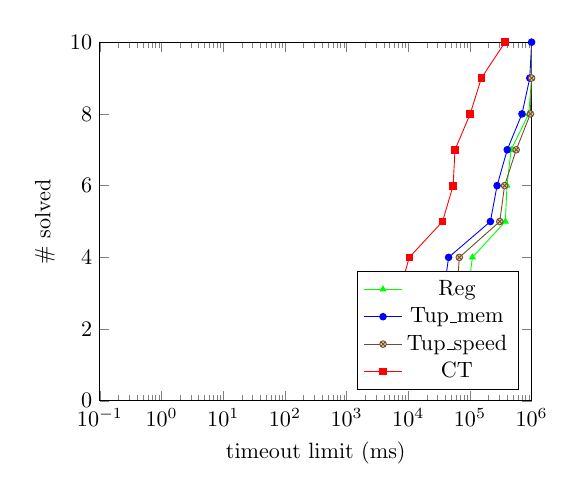
\begin{tikzpicture}[scale=0.8]
      \begin{axis}[
    xmode=log,
    ymin=0,ymax=10,
    xmin=0.1, xmax=1000000,
    every axis plot/.style={thin},
    xlabel={timeout limit (ms)},
    ylabel={\# solved},
    legend pos=south east
    % table/create on use/cumulative distribution/.style={
    %   create col/expr={\pgfmathaccuma + \thisrow{f(x)}}   
    % }
    ]
    \addplot 
    [mark=triangle*,
    mark size=1.5,
    mark options={solid},
    green] 
    coordinates {(31574.208, 1)
(89069.596, 2)
(92409.911, 3)
(109617.692, 4)
(375120.195, 5)
(398745.546, 6)
(464795.600, 7)
(896628.914, 8)
(1000000.519, 9)
(1000001.313, 10)};

    \addplot 
    [blue,
    mark=*,
    mark size=1.5,
    mark options={solid}]
    coordinates {(27237.714, 1)
(35441.131, 2)
(37441.293, 3)
(45077.352, 4)
(214515.372, 5)
(275244.504, 6)
(402643.388, 7)
(697541.797, 8)
(934131.437, 9)
(1000000.647, 10)};

    \addplot [brown!60!black,
    mark options={fill=brown!40},
    mark=otimes*,
    mark size=1.5]
    coordinates {(27847.614, 1)
(43395.528, 2)
(61320.788, 3)
(67245.864, 4)
(304719.299, 5)
(364282.419, 6)
(562899.918, 7)
(955072.437, 8)
(1000000.276, 9)
(1000185.158, 10)};

    \addplot 
    [red,
    mark size=1.5,
    mark=square*]
    coordinates {(4559.768, 1)
(5269.384, 2)
(7089.864, 3)
(10389.645, 4)
(35953.097, 5)
(53378.404, 6)
(57293.505, 7)
(100925.480, 8)
(153336.848, 9)
(371551.862, 10)};
    \legend{Reg,Tup\_mem,Tup\_speed,CT}
  \end{axis}

    \end{tikzpicture}
    \vfill
    \caption{\textbf{Rands JC5000.} The 10 instances of this benchmark
      contain constraints of arity 7. The variable domains are 0..7.}
    \label{fig:simple2}
    \vspace{\baselineskip}
  \end{minipage}\qquad

  \begin{minipage}[b][10cm][s]{.45\textwidth}
    \centering
    \vfill
    \begin{tikzpicture}[scale=0.8]
      \begin{tikzpicture}[scale=1.0]
  \begin{axis}[
    xmode=log,
    ymin=0,ymax=10,
    xmin=0.1, xmax=1000000,
    every axis plot/.style={thin},
    xlabel={timeout limit (ms)},
    ylabel={\# solved},
    legend pos=south east
    % table/create on use/cumulative distribution/.style={
    %   create col/expr={\pgfmathaccuma + \thisrow{f(x)}}   
    % }
    ]
    \addplot 
    [mark=triangle*,
    mark size=1.5,
    mark options={solid},
    green] 
    coordinates {139268.423 1
140601.911 2
177941.502 3
424666.930 4
1000000.472 5
1000000.888 6
1000001.221 7
1000001.407 8
1000001.457 9
1000003.369 10};

    \addplot 
    [blue,
    mark=*,
    mark size=1.5,
    mark options={solid}]
    coordinates {87932.493 1
117877.394 2
124316.924 3
273988.271 4
850622.333 5
1000000.839 6
1000001.004 7
1000001.005 8
1000001.889 9
1000002.453 10};

    \addplot [brown!60!black,
    mark options={fill=brown!40},
    mark=otimes*,
    mark size=1.5]
    table {122789.372 1
146789.073 2
167882.645 3
363255.524 4
1000000.384 5
1000001.258 6
1000002.593 7
1000002.808 8
1000003.164 9
1000004.253 10};

    \addplot 
    [red,
    mark size=1.5,
    mark=square*]
    table {11372.849 1
16562.793 2
18623.245 3
39394.203 4
121998.328 5
124778.898 6
201796.350 7
436664.869 8
954480.066 9
1000000.181 10};
    \legend{Reg,Tup\_mem,Tup\_speed,CT}
  \end{axis}
\end{tikzpicture}

    \end{tikzpicture}
    \vfill
    \caption{\textbf{Rands JC7500}. The 10 instances of this benchmark
      contain constraints of arity 7. The variable domains are 0..7.}
    \vspace{\baselineskip}
  \end{minipage}\qquad
  \begin{minipage}[b][10cm][s]{.45\textwidth}
    \centering
    \vfill
    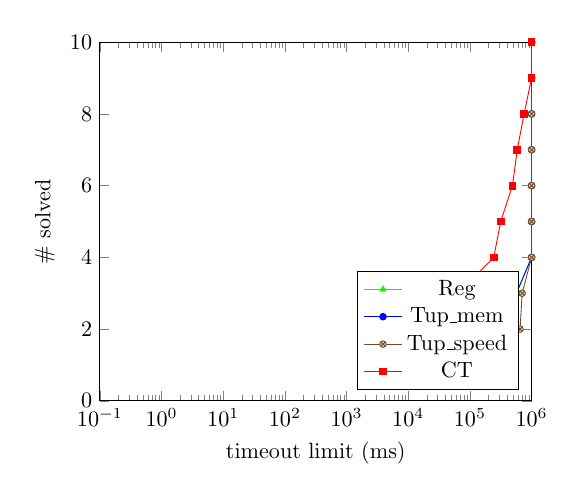
\begin{tikzpicture}[scale=0.8]
      \begin{axis}[
    xmode=log,
    ymin=0,ymax=10,
    xmin=0.1, xmax=1000000,
    every axis plot/.style={thin},
    xlabel={timeout limit (ms)},
    ylabel={\# solved},
    legend pos=south east
    % table/create on use/cumulative distribution/.style={
    %   create col/expr={\pgfmathaccuma + \thisrow{f(x)}}   
    % }
    ]
    \addplot 
    [mark=triangle*,
    mark size=1.5,
    mark options={solid},
    green] 
    coordinates {(332745.543, 1)
(523863.709, 2)
(569686.426, 3)
(1000000.172, 4)
(1000000.554, 5)
(1000000.920, 6)
(1000001.037, 7)
(1000001.490, 8)
(1000002.276, 9)
(1000003.312, 10)};

    \addplot 
    [blue,
    mark=*,
    mark size=1.5,
    mark options={solid}]
    coordinates {(226152.398, 1)
(491387.804, 2)
(566477.841, 3)
(1000000.822, 4)
(1000001.468, 5)
(1000001.597, 6)
(1000001.921, 7)
(1000002.047, 8)
(1000002.465, 9)
(1000003.238, 10)};

    \addplot [brown!60!black,
    mark options={fill=brown!40},
    mark=otimes*,
    mark size=1.5]
    coordinates {(294414.233, 1)
(649951.472, 2)
(702865.808, 3)
(1000000.517, 4)
(1000000.699, 5)
(1000000.802, 6)
(1000001.295, 7)
(1000001.350, 8)
(1000001.480, 9)
(1000001.637, 10)};

    \addplot 
    [red,
    mark size=1.5,
    mark=square*]
    coordinates {(25774.100, 1)
(57124.920, 2)
(64359.631, 3)
(243389.037, 4)
(315549.601, 5)
(489096.976, 6)
(584890.320, 7)
(755476.499, 8)
(1000000.186, 9)
(1000000.225, 10)};
    \legend{Reg,Tup\_mem,Tup\_speed,CT}
  \end{axis}

    \end{tikzpicture}
    \vfill
    \caption{\textbf{Rands JC10000}. The 10 instances of this benchmark
      contain constraints of arity 7. The variable domains are 0..7.}
    \vspace{\baselineskip}
  \end{minipage}\qquad

\end{figure}

\newpage

\begin{figure}
  
  \begin{minipage}[b][10cm][s]{0.45\textwidth}
    \centering
    \vfill
    \begin{tikzpicture}[scale=0.8]
      \begin{tikzpicture}[scale=1.0]
  \begin{axis}[
    xmode=log,
    ymin=0,ymax=23,
    xmin=0.1, xmax=1000000,
    every axis plot/.style={thin},
    xlabel={timeout limit (ms)},
    ylabel={\# solved},
    legend pos=south east
    % table/create on use/cumulative distribution/.style={
    %   create col/expr={\pgfmathaccuma + \thisrow{f(x)}}   
    % }
    ]
    \addplot 
    [mark=triangle*,
    mark size=1.5,
    mark options={solid},
    green] 
    coordinates {0.390 1
0.407 2
0.408 3
0.429 4
0.449 5
0.454 6
0.474 7
0.490 8
0.492 9
0.495 10
0.498 11
0.502 12
0.513 13
0.530 14
0.554 15
0.757 16
0.759 17
1.097 18
1.538 19
1.686 20
1.847 21
4.286 22
5.242 23};

    \addplot 
    [blue,
    mark=*,
    mark size=1.5,
    mark options={solid}]
    coordinates {0.431 1
0.706 2
0.742 3
0.771 4
1.021 5
1.885 6
1.911 7
2.208 8
3.074 9
3.167 10
4.797 11
11.430 12
19.852 13
62.120 14
72.766 15
90.320 16
191.654 17
227.574 18
297.702 19
497.460 20
2463.091 21
4400.894 22
7429.957 23};

    \addplot [brown!60!black,
    mark options={fill=brown!40},
    mark=otimes*,
    mark size=1.5]
    table {0.550 1
0.766 2
0.908 3
0.977 4
1.486 5
2.681 6
2.965 7
3.453 8
4.528 9
4.746 10
7.309 11
17.587 12
30.902 13
90.208 14
106.065 15
137.677 16
291.910 17
340.514 18
456.452 19
743.107 20
3772.207 21
6539.383 22
11517.655 23};

    \addplot 
    [red,
    mark size=1.5,
    mark=square*]
    table {0.439 1
0.618 2
0.698 3
0.735 4
1.093 5
1.910 6
2.099 7
2.368 8
2.794 9
3.010 10
4.795 11
11.303 12
19.709 13
53.169 14
61.288 15
66.296 16
156.013 17
182.439 18
253.668 19
338.968 20
1947.380 21
2773.622 22
4557.056 23};
    \legend{Reg,Tup\_mem,Tup\_speed,CT}
  \end{axis}
\end{tikzpicture}

    \end{tikzpicture}
    \vfill
    \caption{\textbf{AIM-50}. The 23 instances
    of this benchmark contain ternary constraints 
    and a few binary constraints. All variables
    are 0/1.}
    \vspace{\baselineskip}
  \end{minipage}\qquad
  \begin{minipage}[b][10cm][s]{0.45\textwidth}
    \centering
    \vfill
    \begin{tikzpicture}[scale=0.8]
      \begin{axis}[
    xmode=log,
    ymin=0,ymax=23,
    xmin=0.1, xmax=1000000,
    every axis plot/.style={thin},
    xlabel={timeout limit (ms)},
    ylabel={\# solved},
    legend pos=south east
    % table/create on use/cumulative distribution/.style={
    %   create col/expr={\pgfmathaccuma + \thisrow{f(x)}}   
    % }
    ]
    \addplot 
    [mark=triangle*,
    mark size=1.5,
    mark options={solid},
    green] 
    coordinates {(0.823, 1)
(0.832, 2)
(0.857, 3)
(0.867, 4)
(0.885, 5)
(0.918, 6)
(0.939, 7)
(0.953, 8)
(0.974, 9)
(0.981, 10)
(0.987, 11)
(0.988, 12)
(1.008, 13)
(1.061, 14)
(1.135, 15)
(1.205, 16)
(2.753, 17)
(3.647, 18)
(24.877, 19)
(24.886, 20)
(35.599, 21)
(42.011, 22)
(48.965, 23)};

    \addplot 
    [blue,
    mark=*,
    mark size=1.5,
    mark options={solid}]
    coordinates {(3.586, 1)
(3.671, 2)
(6.004, 3)
(9.450, 4)
(15.887, 5)
(52.426, 6)
(80.095, 7)
(171.902, 8)
(4436.194, 9)
(41949.006, 10)
(100934.221, 11)
(147492.566, 12)
(556004.535, 13)
(1000000.165, 14)
(1000000.167, 15)
(1000000.174, 16)
(1000000.174, 17)
(1000000.176, 18)
(1000000.179, 19)
(1000000.202, 20)
(1000000.260, 21)
(1000000.266, 22)
(1000000.286, 23)};

    \addplot [brown!60!black,
    mark options={fill=brown!40},
    mark=otimes*,
    mark size=1.5]
    table {(5.211, 1)
(5.793, 2)
(9.033, 3)
(13.782, 4)
(24.369, 5)
(77.669, 6)
(120.860, 7)
(258.984, 8)
(6933.488, 9)
(65101.206, 10)
(165079.465, 11)
(242773.103, 12)
(877436.255, 13)
(1000000.113, 14)
(1000000.118, 15)
(1000000.123, 16)
(1000000.132, 17)
(1000000.154, 18)
(1000000.165, 19)
(1000000.189, 20)
(1000000.191, 21)
(1000000.196, 22)
(1000000.259, 23)};

    \addplot 
    [red,
    mark size=1.5,
    mark=square*]
    table {(3.886, 1)
(4.643, 2)
(6.772, 3)
(11.080, 4)
(17.750, 5)
(62.656, 6)
(87.179, 7)
(187.117, 8)
(4632.128, 9)
(36310.893, 10)
(96431.551, 11)
(140762.037, 12)
(452408.039, 13)
(1000000.102, 14)
(1000000.115, 15)
(1000000.118, 16)
(1000000.134, 17)
(1000000.137, 18)
(1000000.157, 19)
(1000000.200, 20)
(1000000.202, 21)
(1000000.221, 22)
(1000000.239, 23)};
    \legend{Reg,Tup\_mem,Tup\_speed,CT}
  \end{axis}

    \end{tikzpicture}
    \vfill
    \caption{\textbf{AIM-100}. The 23 instances
      of this benchmark contain ternary constraints 
      and a few binary constraints. All variables
      are 0/1.}
    \vspace{\baselineskip}
  \end{minipage}\qquad
  \begin{minipage}[b][10cm][s]{0.45\textwidth}
    \centering
    \vfill
    \begin{tikzpicture}[scale=0.8]
      \begin{axis}[
    xmode=log,
    ymin=0,ymax=22,
    xmin=0.1, xmax=1000000,
    every axis plot/.style={thin},
    xlabel={timeout limit (ms)},
    ylabel={\# solved},
    legend pos=south east
    % table/create on use/cumulative distribution/.style={
    %   create col/expr={\pgfmathaccuma + \thisrow{f(x)}}   
    % }
    ]
    \addplot 
    [mark=triangle*,
    mark size=1.5,
    mark options={solid},
    green] 
    coordinates {(2.092, 1)
(2.153, 2)
(2.207, 3)
(2.224, 4)
(2.353, 5)
(2.410, 6)
(2.444, 7)
(2.462, 8)
(2.486, 9)
(2.626, 10)
(2.638, 11)
(4.751, 12)
(7.714, 13)
(12.349, 14)
(459.348, 15)
(786.654, 16)
(1926.845, 17)
(7178.726, 18)
(13920.549, 19)
(63961.995, 20)
(83629.587, 21)
(215920.851, 22)};

    \addplot 
    [blue,
    mark=*,
    mark size=1.5,
    mark options={solid}]
    coordinates {(92.762, 1)
(214.140, 2)
(5059.466, 3)
(9347.039, 4)
(1000000.212, 5)
(1000000.214, 6)
(1000000.230, 7)
(1000000.234, 8)
(1000000.236, 9)
(1000000.243, 10)
(1000000.247, 11)
(1000000.332, 12)
(1000000.348, 13)
(1000000.356, 14)
(1000000.384, 15)
(1000000.413, 16)
(1000000.580, 17)
(1001526.960, 18)
(1013587.491, 19)
(1015726.858, 20)
(1021700.000, 21)
(1026780.972, 22)};

    \addplot [brown!60!black,
    mark options={fill=brown!40},
    mark=otimes*,
    mark size=1.5]
    table {(144.623, 1)
(333.321, 2)
(9960.406, 3)
(14839.411, 4)
(1000000.132, 5)
(1000000.132, 6)
(1000000.138, 7)
(1000000.154, 8)
(1000000.156, 9)
(1000000.161, 10)
(1000000.176, 11)
(1000000.201, 12)
(1000000.233, 13)
(1000000.233, 14)
(1000000.264, 15)
(1000000.302, 16)
(1000000.338, 17)
(1000000.401, 18)
(1000000.462, 19)
(1000000.559, 20)
(1000201.313, 21)
(1030367.681, 22)};

    \addplot 
    [red,
    mark size=1.5,
    mark=square*]
    table {(120.173, 1)
(264.364, 2)
(6492.284, 3)
(12332.389, 4)
(1000000.117, 5)
(1000000.130, 6)
(1000000.138, 7)
(1000000.141, 8)
(1000000.144, 9)
(1000000.148, 10)
(1000000.157, 11)
(1000000.179, 12)
(1000000.199, 13)
(1000000.223, 14)
(1000000.258, 15)
(1000000.312, 16)
(1000000.349, 17)
(1000000.387, 18)
(1000000.408, 19)
(1019145.714, 20)
(1021004.571, 21)
(1051023.598, 22)};
    \legend{Reg,Tup\_mem,Tup\_speed,CT}
  \end{axis}

    \end{tikzpicture}
    \vfill
    \caption{\textbf{AIM-200}. The 22 instances
    of this benchmark contain contain ternary constraints 
    and a few binary constraints. All variables
    are 0/1.}
    \vspace{\baselineskip}
  \end{minipage}\qquad
\end{figure}

\newpage

\begin{figure}
  \begin{minipage}[b][10cm][s]{0.45\textwidth}
    \centering
    \vfill
    \begin{tikzpicture}[scale=0.8]
      \begin{tikzpicture}[scale=1.0]
  \begin{axis}[
    xmode=log,
    ymin=0,ymax=50,
    xmin=0.1, xmax=1000000,
    every axis plot/.style={thin},
    xlabel={timeout limit (ms)},
    ylabel={\# solved},
    legend pos=south east
    % table/create on use/cumulative distribution/.style={
    %   create col/expr={\pgfmathaccuma + \thisrow{f(x)}}   
    % }
    ]
    \addplot 
    [mark=triangle*,
    mark size=1.5,
    mark options={solid},
    green] 
    coordinates {21539.047 1
23631.895 2
23716.403 3
24241.194 4
24452.383 5
24702.581 6
24727.049 7
24735.421 8
24762.823 9
25381.219 10
25446.865 11
25447.244 12
25663.048 13
25681.411 14
25705.552 15
25921.922 16
26000.936 17
26206.810 18
26236.781 19
26242.879 20
26255.926 21
26263.647 22
26276.749 23
26572.969 24
26580.275 25
26658.352 26
26798.498 27
27134.428 28
27340.416 29
27401.714 30
27486.019 31
27561.142 32
27728.713 33
27922.916 34
28054.949 35
28057.644 36
28193.151 37
28328.067 38
28495.760 39
28577.913 40
28589.075 41
28945.618 42
29006.507 43
29341.039 44
29520.154 45
29560.978 46
29585.618 47
29688.054 48
29934.812 49
30055.889 50};

    \addplot 
    [blue,
    mark=*,
    mark size=1.5,
    mark options={solid}]
    coordinates {7672.186 1
7964.072 2
7988.188 3
8311.150 4
8326.644 5
8405.755 6
8413.912 7
8433.367 8
8543.205 9
8852.685 10
8991.001 11
9027.728 12
9120.668 13
9300.145 14
9307.344 15
9334.373 16
9427.760 17
9445.763 18
9469.390 19
9514.190 20
9600.928 21
9650.273 22
9746.749 23
9808.637 24
9817.477 25
9908.257 26
9966.772 27
9974.917 28
10107.698 29
10130.344 30
10214.500 31
10354.798 32
10411.441 33
10412.120 34
10566.980 35
10629.555 36
10690.029 37
10750.761 38
10771.949 39
10783.994 40
10796.075 41
10819.530 42
10910.396 43
10935.039 44
11189.948 45
11409.743 46
11725.089 47
11914.318 48
12087.322 49
12551.558 50};

    \addplot [brown!60!black,
    mark options={fill=brown!40},
    mark=otimes*,
    mark size=1.5]
    table {11083.294 1
11942.343 2
12057.186 3
12065.914 4
12165.546 5
12230.996 6
12353.178 7
12499.801 8
12539.423 9
12659.462 10
12724.767 11
12772.533 12
13125.773 13
13328.450 14
13638.694 15
13680.520 16
13726.853 17
13788.117 18
13799.316 19
13929.021 20
13937.426 21
14037.418 22
14066.707 23
14101.725 24
14130.306 25
14152.192 26
14478.238 27
14540.951 28
14544.138 29
14609.419 30
14697.861 31
14702.186 32
14899.661 33
15027.878 34
15089.663 35
15146.606 36
15213.444 37
15229.658 38
15372.915 39
15428.330 40
15796.160 41
15805.142 42
15904.232 43
16049.472 44
16141.290 45
16151.591 46
16160.955 47
16942.804 48
17001.615 49
17047.240 50};

    \addplot 
    [red,
    mark size=1.5,
    mark=square*]
    table {2427.974 1
2699.046 2
2717.750 3
2743.960 4
2797.776 5
2816.502 6
2841.334 7
2900.942 8
2904.804 9
2908.160 10
2910.491 11
2933.117 12
2933.400 13
2967.383 14
2989.519 15
3003.038 16
3029.964 17
3063.311 18
3093.973 19
3141.933 20
3150.100 21
3186.832 22
3220.475 23
3234.416 24
3239.493 25
3269.265 26
3293.108 27
3353.966 28
3379.302 29
3394.468 30
3439.955 31
3458.748 32
3527.174 33
3528.582 34
3540.231 35
3558.883 36
3570.218 37
3574.549 38
3610.825 39
3624.569 40
3627.753 41
3673.298 42
3729.990 43
3743.274 44
3779.422 45
3788.515 46
3859.838 47
3898.223 48
3979.624 49
4133.050 50};
    \legend{Reg,Tup\_mem,Tup\_speed,CT}
  \end{axis}
\end{tikzpicture}

    \end{tikzpicture}
    \vfill
    \caption{\textbf{A5}. The 50 instances
      of this benchmark contain constraints of arity 5.
      The variables are 0/1.}
    \vspace{\baselineskip}
  \end{minipage}\qquad

  \begin{minipage}[b][10cm][s]{0.45\textwidth}
    \centering
    \vfill
    \begin{tikzpicture}[scale=0.8]
      \begin{tikzpicture}[scale=1.0]
  \begin{axis}[
    xmode=log,
    ymin=0,ymax=23,
    xmin=0.1, xmax=1000000,
    every axis plot/.style={thin},
    xlabel={timeout limit (ms)},
    ylabel={\# solved},
    legend pos=south east
    % table/create on use/cumulative distribution/.style={
    %   create col/expr={\pgfmathaccuma + \thisrow{f(x)}}   
    % }
    ]
    \addplot 
    [mark=triangle*,
    mark size=1.5,
    mark options={solid},
    green] 
    coordinates {727435.433 1
1000001.373 2
1000005.483 3
1000006.809 4
1000008.096 5
1000009.635 6
1000010.074 7
1000011.271 8
1000012.432 9
1000012.672 10
1000015.905 11
1000017.026 12
1000022.231 13
1000029.449 14
1000030.270 15
1000031.062 16
1000036.397 17
1000036.748 18
1000039.103 19
1000043.823 20
1000044.070 21
1000052.767 22
1000080.677 23};

    \addplot 
    [blue,
    mark=*,
    mark size=1.5,
    mark options={solid}]
    coordinates {224520.942 1
311434.541 2
518531.192 3
563843.176 4
816767.503 5
1000001.025 6
1000001.573 7
1000003.413 8
1000003.543 9
1000003.636 10
1000004.219 11
1000005.825 12
1000006.947 13
1000008.010 14
1000009.980 15
1000012.435 16
1000015.261 17
1000015.833 18
1000017.025 19
1000023.640 20
1000029.233 21
1000041.787 22
1000054.453 23};

    \addplot [brown!60!black,
    mark options={fill=brown!40},
    mark=otimes*,
    mark size=1.5]
    table {316710.534 1
410461.377 2
648720.274 3
713048.102 4
1000002.616 5
1000004.304 6
1000005.477 7
1000005.720 8
1000009.313 9
1000010.227 10
1000014.478 11
1000014.751 12
1000020.934 13
1000021.694 14
1000022.834 15
1000022.849 16
1000028.045 17
1000028.187 18
1000031.847 19
1000032.588 20
1000032.896 21
1000044.704 22
1000046.876 23};

    \addplot 
    [red,
    mark size=1.5,
    mark=square*]
    table {20486.588 1
58503.164 2
61130.226 3
77146.092 4
94763.488 5
153385.993 6
226208.408 7
402373.676 8
417665.968 9
446212.851 10
455410.096 11
600725.556 12
1000000.185 13
1000000.197 14
1000000.502 15
1000000.985 16
1000001.080 17
1000001.500 18
1000001.515 19
1000001.657 20
1000002.297 21
1000002.778 22
1000003.801 23};
    \legend{Reg,Tup\_mem,Tup\_speed,CT}
  \end{axis}
\end{tikzpicture}

    \end{tikzpicture}
    \vfill
    \caption{\textbf{A10}. The 50 instances
    of this benchmark contain constraints of arity X.
    Most of the variables are 0/1, and some are
    singletons.}
    \vspace{\baselineskip}
  \end{minipage}\qquad
\end{figure}

\newpage

\begin{figure}
  \begin{minipage}[b][10cm][s]{0.45\textwidth}
    \centering
    \vfill
    \begin{tikzpicture}[scale=0.8]
      \begin{tikzpicture}[scale=1.0]
  \begin{axis}[
    xmode=log,
    ymin=0,ymax=65,
    xmin=0.1, xmax=1000000,
    every axis plot/.style={thin},
    xlabel={timeout limit (ms)},
    ylabel={\# solved},
    legend pos=south east
    % table/create on use/cumulative distribution/.style={
    %   create col/expr={\pgfmathaccuma + \thisrow{f(x)}}   
    % }
    ]
    \addplot 
    [mark=triangle*,
    mark size=1.5,
    mark options={solid},
    green] 
    coordinates {0.078 1
0.089 2
0.089 3
0.093 4
0.094 5
0.095 6
0.095 7
0.097 8
0.098 9
0.098 10
0.099 11
0.099 12
0.099 13
0.102 14
0.103 15
0.103 16
0.106 17
0.157 18
0.831 19
1.490 20
1.498 21
1.518 22
1.954 23
3.734 24
3.737 25
4.347 26
9.191 27
10.580 28
19.169 29
22.780 30
26.266 31
81.558 32
102.447 33
104.991 34
131.512 35
332.462 36
352.388 37
618.827 38
788.523 39
790.494 40
1259.350 41
1678.432 42
1862.544 43
2455.933 44
2837.051 45
3271.878 46
4855.913 47
6934.464 48
7463.727 49
8049.052 50
8952.593 51
19737.517 52
23132.443 53
23469.266 54
26002.371 55
29111.360 56
42946.710 57
73225.089 58
74320.226 59
75593.251 60
108672.990 61
122929.922 62
149958.110 63
163565.715 64
261688.209 65};

    \addplot 
    [blue,
    mark=*,
    mark size=1.5,
    mark options={solid}]
    coordinates {0.342 1
0.351 2
0.361 3
0.400 4
0.401 5
0.420 6
0.433 7
0.433 8
0.436 9
0.442 10
0.476 11
0.489 12
0.492 13
0.493 14
0.549 15
0.590 16
0.652 17
0.720 18
0.923 19
1.008 20
1.184 21
1.528 22
1.727 23
2.724 24
3.600 25
7.208 26
7.829 27
8.978 28
12.102 29
17.784 30
33.887 31
40.219 32
55.846 33
61.501 34
164.731 35
184.236 36
360.816 37
429.133 38
484.976 39
586.591 40
794.649 41
932.019 42
1474.042 43
1555.417 44
1890.818 45
3795.101 46
5347.478 47
6026.047 48
7463.682 49
9392.594 50
12105.731 51
25050.002 52
40536.372 53
48045.798 54
61824.891 55
74212.070 56
143995.198 57
243803.619 58
296870.468 59
302900.312 60
322459.873 61
333997.695 62
444619.255 63
457064.862 64
908177.605 65};

    \addplot [brown!60!black,
    mark options={fill=brown!40},
    mark=otimes*,
    mark size=1.5]
    table {0.702 1
0.797 2
0.808 3
0.911 4
0.944 5
0.954 6
0.961 7
1.001 8
1.027 9
1.096 10
1.103 11
1.108 12
1.156 13
1.178 14
1.190 15
1.198 16
1.218 17
1.346 18
1.419 19
1.807 20
2.596 21
3.899 22
4.099 23
5.733 24
5.889 25
9.553 26
10.532 27
11.796 28
28.281 29
29.933 30
49.328 31
75.166 32
103.942 33
120.948 34
278.999 35
367.701 36
427.636 37
574.683 38
660.416 39
802.131 40
1091.373 41
1360.532 42
1932.804 43
2291.232 44
2682.220 45
5395.569 46
7382.573 47
8090.518 48
8788.504 49
12047.370 50
15892.962 51
30283.964 52
52697.241 53
60018.686 54
76459.238 55
87041.593 56
184487.102 57
286328.868 58
338304.442 59
353888.532 60
366508.306 61
398389.231 62
531168.118 63
545050.662 64
1000001.713 65};

    \addplot 
    [red,
    mark size=1.5,
    mark=square*]
    table {0.069 1
0.069 2
0.080 3
0.086 4
0.086 5
0.089 6
0.089 7
0.089 8
0.090 9
0.091 10
0.092 11
0.092 12
0.093 13
0.093 14
0.094 15
0.096 16
0.099 17
0.101 18
0.365 19
0.406 20
0.422 21
0.510 22
0.784 23
1.236 24
1.591 25
1.712 26
1.824 27
2.622 28
5.997 29
6.538 30
7.745 31
17.398 32
24.309 33
26.727 34
33.697 35
63.005 36
63.138 37
77.013 38
147.914 39
162.476 40
176.882 41
296.947 42
330.613 43
459.449 44
472.783 45
804.999 46
1061.529 47
1140.902 48
1254.905 49
1867.303 50
2462.669 51
4400.046 52
8169.387 53
9165.590 54
9457.464 55
9850.643 56
23517.073 57
36089.500 58
38817.645 59
40027.459 60
47404.529 61
50511.047 62
64207.992 63
70129.605 64
130009.590 65};
    \legend{Reg,Tup\_mem,Tup\_speed,CT}
  \end{axis}
\end{tikzpicture}

    \end{tikzpicture}
    \vfill
    \caption{\textbf{Crosswords WorldVG}.
    The 65 instances of this benchmark contain 
    constraints of arities ranging from 2 to 20. 
    The variable domains are 0..25.}
    \vspace{\baselineskip}
  \end{minipage}\qquad

    \begin{minipage}[b][10cm][s]{0.45\textwidth}
    \centering
    \vfill
    \begin{tikzpicture}[scale=0.8]
      \begin{axis}[
    xmode=log,
    ymin=0,ymax=63,
    xmin=0.1, xmax=1000000,
    every axis plot/.style={thin},
    xlabel={timeout limit (ms)},
    ylabel={\# solved},
    legend pos=south east
    % table/create on use/cumulative distribution/.style={
    %   create col/expr={\pgfmathaccuma + \thisrow{f(x)}}   
    % }
    ]
    \addplot 
    [mark=triangle*,
    mark size=1.5,
    mark options={solid},
    green] 
    coordinates {(0.074, 1)
(0.076, 2)
(0.078, 3)
(0.082, 4)
(0.089, 5)
(0.089, 6)
(0.092, 7)
(0.096, 8)
(0.097, 9)
(0.097, 10)
(0.097, 11)
(0.099, 12)
(0.099, 13)
(0.102, 14)
(0.103, 15)
(0.108, 16)
(0.117, 17)
(0.123, 18)
(0.500, 19)
(0.676, 20)
(0.723, 21)
(0.905, 22)
(1.332, 23)
(1.692, 24)
(1.766, 25)
(1.791, 26)
(5.276, 27)
(16.858, 28)
(17.927, 29)
(30.069, 30)
(35.255, 31)
(41.801, 32)
(52.490, 33)
(75.080, 34)
(96.307, 35)
(130.683, 36)
(131.067, 37)
(225.774, 38)
(274.112, 39)
(379.638, 40)
(550.637, 41)
(909.264, 42)
(1274.166, 43)
(1388.373, 44)
(2525.152, 45)
(2533.498, 46)
(2595.853, 47)
(4030.753, 48)
(4547.362, 49)
(5055.465, 50)
(5791.415, 51)
(10242.753, 52)
(12298.425, 53)
(14360.436, 54)
(14982.830, 55)
(17458.388, 56)
(20992.013, 57)
(29908.599, 58)
(33944.527, 59)
(36060.331, 60)
(55002.467, 61)
(60672.239, 62)
(76112.252, 63)};

    \addplot 
    [blue,
    mark=*,
    mark size=1.5,
    mark options={solid}]
    coordinates {(0.273, 1)
(0.276, 2)
(0.280, 3)
(0.282, 4)
(0.283, 5)
(0.284, 6)
(0.299, 7)
(0.306, 8)
(0.311, 9)
(0.319, 10)
(0.323, 11)
(0.345, 12)
(0.352, 13)
(0.399, 14)
(0.502, 15)
(0.503, 16)
(0.531, 17)
(0.536, 18)
(0.570, 19)
(0.573, 20)
(0.880, 21)
(1.282, 22)
(1.284, 23)
(1.298, 24)
(1.740, 25)
(2.601, 26)
(3.676, 27)
(4.898, 28)
(9.614, 29)
(9.646, 30)
(17.588, 31)
(26.301, 32)
(53.031, 33)
(63.457, 34)
(140.413, 35)
(155.119, 36)
(167.139, 37)
(223.250, 38)
(272.924, 39)
(302.082, 40)
(761.487, 41)
(945.499, 42)
(1346.690, 43)
(1449.372, 44)
(1491.881, 45)
(2704.616, 46)
(3119.614, 47)
(5009.739, 48)
(5632.408, 49)
(7755.518, 50)
(8079.373, 51)
(13953.623, 52)
(17063.131, 53)
(19618.816, 54)
(21960.324, 55)
(24240.394, 56)
(39633.214, 57)
(64699.544, 58)
(71580.728, 59)
(73166.699, 60)
(112247.995, 61)
(121257.043, 62)
(151915.668, 63)};

    \addplot [brown!60!black,
    mark options={fill=brown!40},
    mark=otimes*,
    mark size=1.5]
    table {(0.412, 1)
(0.457, 2)
(0.458, 3)
(0.464, 4)
(0.471, 5)
(0.484, 6)
(0.496, 7)
(0.516, 8)
(0.572, 9)
(0.572, 10)
(0.598, 11)
(0.679, 12)
(0.734, 13)
(0.864, 14)
(1.027, 15)
(1.106, 16)
(1.203, 17)
(1.280, 18)
(1.557, 19)
(1.667, 20)
(2.002, 21)
(2.016, 22)
(2.303, 23)
(2.819, 24)
(2.952, 25)
(2.970, 26)
(5.162, 27)
(5.506, 28)
(18.023, 29)
(19.081, 30)
(39.969, 31)
(56.794, 32)
(100.167, 33)
(128.098, 34)
(172.182, 35)
(249.519, 36)
(259.430, 37)
(286.138, 38)
(488.848, 39)
(568.244, 40)
(1062.970, 41)
(1350.822, 42)
(1626.744, 43)
(1729.003, 44)
(2145.034, 45)
(3496.611, 46)
(3833.896, 47)
(6131.314, 48)
(7395.849, 49)
(9657.251, 50)
(10635.431, 51)
(17957.948, 52)
(19794.735, 53)
(25594.928, 54)
(27375.416, 55)
(30057.643, 56)
(50552.660, 57)
(78826.698, 58)
(88585.449, 59)
(90256.706, 60)
(134279.170, 61)
(143593.547, 62)
(181192.715, 63)};

    \addplot 
    [red,
    mark size=1.5,
    mark=square*]
    table {(0.068, 1)
(0.068, 2)
(0.069, 3)
(0.070, 4)
(0.072, 5)
(0.073, 6)
(0.073, 7)
(0.075, 8)
(0.077, 9)
(0.080, 10)
(0.081, 11)
(0.084, 12)
(0.087, 13)
(0.087, 14)
(0.088, 15)
(0.088, 16)
(0.089, 17)
(0.090, 18)
(0.091, 19)
(0.093, 20)
(0.350, 21)
(0.416, 22)
(0.568, 23)
(0.568, 24)
(0.626, 25)
(0.803, 26)
(1.154, 27)
(1.608, 28)
(4.334, 29)
(4.592, 30)
(9.543, 31)
(14.146, 32)
(20.935, 33)
(24.430, 34)
(31.227, 35)
(39.168, 36)
(59.321, 37)
(71.346, 38)
(116.614, 39)
(120.688, 40)
(172.687, 41)
(207.521, 42)
(217.931, 43)
(266.423, 44)
(477.466, 45)
(566.003, 46)
(683.586, 47)
(1064.142, 48)
(1232.853, 49)
(1672.169, 50)
(1747.561, 51)
(2681.469, 52)
(2811.215, 53)
(4092.535, 54)
(4387.910, 55)
(5269.595, 56)
(8047.345, 57)
(14122.235, 58)
(14686.169, 59)
(14970.167, 60)
(19502.734, 61)
(26550.723, 62)
(32323.306, 63)};
    \legend{Reg,Tup\_mem,Tup\_speed,CT}
  \end{axis}

    \end{tikzpicture}
    \vfill
    \caption{\textbf{Crosswords LexVG}.
    The 63 instances of this benchmark contain
    constraints of arity from 5 to 20. 
    Variable domains are 0..25.}
    \vspace{\baselineskip}
  \end{minipage}\qquad
  \begin{minipage}[b][10cm][s]{0.45\textwidth}
    \centering
    \vfill
    \begin{tikzpicture}[scale=0.8]
      \begin{tikzpicture}[scale=1.0]
  \begin{axis}[
    xmode=log,
    ymin=0,ymax=22,
    xmin=0.1, xmax=1000000,
    every axis plot/.style={thin},
    xlabel={timeout limit (ms)},
    ylabel={\# solved},
    legend pos=south east
    % table/create on use/cumulative distribution/.style={
    %   create col/expr={\pgfmathaccuma + \thisrow{f(x)}}   
    % }
    ]
    \addplot 
    [mark=triangle*,
    mark size=1.5,
    mark options={solid},
    green] 
    coordinates {0.150 1
0.382 2
1.156 3
1.231 4
1.662 5
1.826 6
2.291 7
2.622 8
5.011 9
8.353 10
9.860 11
15.302 12
18.579 13
22.834 14
27.862 15
29.816 16
36.345 17
45.878 18
285.224 19
1131.791 20
1278.079 21
2204.696 22};

    \addplot 
    [blue,
    mark=*,
    mark size=1.5,
    mark options={solid}]
    coordinates {0.138 1
0.311 2
0.790 3
1.624 4
1.760 5
1.791 6
2.063 7
3.631 8
4.094 9
4.213 10
5.035 11
5.357 12
6.556 13
6.847 14
9.371 15
11.612 16
16.633 17
18.028 18
42.410 19
175.300 20
4664.842 21
193998.166 22};

    \addplot [brown!60!black,
    mark options={fill=brown!40},
    mark=otimes*,
    mark size=1.5]
    table {0.146 1
0.391 2
0.855 3
1.897 4
1.958 5
2.033 6
2.272 7
4.342 8
4.459 9
4.946 10
5.389 11
5.697 12
7.018 13
7.259 14
10.784 15
12.976 16
20.478 17
20.679 18
41.775 19
49.515 20
218.327 21
246737.472 22};

    \addplot 
    [red,
    mark size=1.5,
    mark=square*]
    table {0.125 1
0.237 2
0.372 3
0.544 4
0.636 5
0.682 6
0.685 7
1.085 8
1.099 9
1.110 10
1.455 11
1.631 12
1.870 13
2.270 14
3.062 15
4.409 16
8.078 17
8.255 18
18.086 19
20.971 20
61.702 21
127890.223 22};
    \legend{Reg,Tup\_mem,Tup\_speed,CT}
  \end{axis}
\end{tikzpicture}

    \end{tikzpicture}
    \vfill
    \caption{\textbf{Crosswords Wordspuzzle}.
      The 22 instances of this benchmark contain 
      constraints of arities ranging from 2 to 13.
      The variable domains are 0..25.}
    \vspace{\baselineskip}
  \end{minipage}\qquad
  
\end{figure}

\newpage

\begin{figure}
    \begin{minipage}[b][10cm][s]{0.45\textwidth}
    \centering
    \vfill
    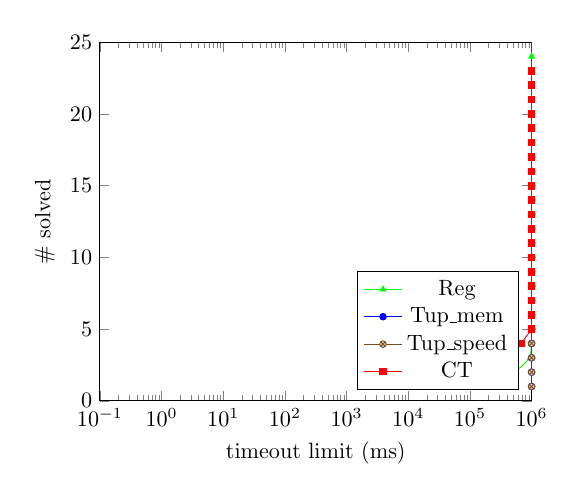
\begin{tikzpicture}[scale=0.8]
      \begin{axis}[
    xmode=log,
    ymin=0,ymax=25,
    xmin=0.1, xmax=1000000,
    every axis plot/.style={thin},
    xlabel={timeout limit (ms)},
    ylabel={\# solved},
    legend pos=south east
    % table/create on use/cumulative distribution/.style={
    %   create col/expr={\pgfmathaccuma + \thisrow{f(x)}}   
    % }
    ]
    \addplot 
    [mark=triangle*,
    mark size=1.5,
    mark options={solid},
    green] 
    coordinates {(362179.365, 1)
(542610.443, 2)
(956273.144, 3)
(1000000.188, 4)
(1000000.201, 5)
(1000000.201, 6)
(1000000.220, 7)
(1000000.266, 8)
(1000000.268, 9)
(1000000.291, 10)
(1000000.294, 11)
(1000000.295, 12)
(1000000.297, 13)
(1000000.329, 14)
(1000000.339, 15)
(1000000.376, 16)
(1000000.377, 17)
(1000000.409, 18)
(1000000.412, 19)
(1000000.463, 20)
(1000000.483, 21)
(1000000.641, 22)
(1000000.668, 23)
(1000000.801, 24)
(1029699.464, 25)};

    \addplot 
    [blue,
    mark=*,
    mark size=1.5,
    mark options={solid}]
    coordinates {(1000001.069, 1)
(1000001.150, 2)
(1000001.274, 3)
(1000001.277, 4)
(1000001.523, 5)
(1000002.056, 6)
(1000002.073, 7)
(1000002.311, 8)
(1000002.579, 9)
(1000002.756, 10)
(1000003.085, 11)
(1000004.834, 12)
(1000004.876, 13)
(1000005.836, 14)
(1000005.855, 15)
(1000006.115, 16)
(1000006.863, 17)
(1000007.924, 18)
(1000008.395, 19)
(1000008.443, 20)
(1000009.040, 21)
(1000013.352, 22)
(1000013.437, 23)
(1000013.463, 24)
(1022769.751, 25)};

    \addplot [brown!60!black,
    mark options={fill=brown!40},
    mark=otimes*,
    mark size=1.5]
    coordinates {(1000000.597, 1)
(1000000.598, 2)
(1000000.770, 3)
(1000000.849, 4)
(1000001.124, 5)
(1000001.175, 6)
(1000001.309, 7)
(1000001.317, 8)
(1000001.461, 9)
(1000001.753, 10)
(1000001.826, 11)
(1000002.114, 12)
(1000002.685, 13)
(1000003.527, 14)
(1000003.580, 15)
(1000003.656, 16)
(1000004.416, 17)
(1000005.342, 18)
(1000006.111, 19)
(1000006.504, 20)
(1000007.848, 21)
(1000009.651, 22)
(1000010.626, 23)
(1000011.794, 24)
(1000016.468, 25)};

    \addplot 
    [red,
    mark size=1.5,
    mark=square*]
    coordinates {(45570.744, 1)
(97963.633, 2)
(284803.058, 3)
(676940.142, 4)
(1000000.180, 5)
(1000000.233, 6)
(1000000.268, 7)
(1000000.271, 8)
(1000000.295, 9)
(1000000.309, 10)
(1000000.312, 11)
(1000000.324, 12)
(1000000.334, 13)
(1000000.347, 14)
(1000000.351, 15)
(1000000.363, 16)
(1000000.386, 17)
(1000000.400, 18)
(1000000.453, 19)
(1000000.503, 20)
(1000000.579, 21)
(1000000.609, 22)
(1000000.673, 23)
(1019921.469, 24)
(1040148.010, 25)};
    \legend{Reg,Tup\_mem,Tup\_speed,CT}
  \end{axis}

    \end{tikzpicture}
    \vfill
    \caption{\textbf{MDD 05}. The 25 instances of this benchmark
    contain constraints of arity $7$. The variable domains
    are 0..4.}
    \vspace{\baselineskip}
  \end{minipage}\qquad
  \begin{minipage}[b][10cm][s]{0.45\textwidth}
    \centering
    \vfill
    \begin{tikzpicture}[scale=0.8]
      \begin{tikzpicture}[scale=1.0]
  \begin{axis}[
    xmode=log,
    ymin=0,ymax=9,
    xmin=0.1, xmax=1000000,
    every axis plot/.style={thin},
    xlabel={timeout limit (ms)},
    ylabel={\# solved},
    legend pos=south east
    % table/create on use/cumulative distribution/.style={
    %   create col/expr={\pgfmathaccuma + \thisrow{f(x)}}   
    % }
    ]
    \addplot 
    [mark=triangle*,
    mark size=1.5,
    mark options={solid},
    green] 
    coordinates {8143.453 1
28227.868 2
30184.398 3
39636.695 4
40458.753 5
56228.579 6
66820.027 7
79866.961 8
245383.866 9};

    \addplot 
    [blue,
    mark=*,
    mark size=1.5,
    mark options={solid}]
    coordinates {1000001.471 1
1000001.544 2
1000002.625 3
1000002.721 4
1000002.899 5
1000003.208 6
1000004.208 7
1000004.650 8
1000005.052 9};

    \addplot [brown!60!black,
    mark options={fill=brown!40},
    mark=otimes*,
    mark size=1.5]
    table {1000000.498 1
1000000.780 2
1000000.821 3
1000001.078 4
1000001.299 5
1000001.505 6
1000002.168 7
1000004.073 8
1000008.854 9};

    \addplot 
    [red,
    mark size=1.5,
    mark=square*]
    table {1000000.160 1
1000000.224 2
1000000.247 3
1000000.259 4
1000000.300 5
1000000.307 6
1000000.343 7
1000000.404 8
1000000.445 9};
    \legend{Reg,Tup\_mem,Tup\_speed,CT}
  \end{axis}
\end{tikzpicture}

    \end{tikzpicture}
    \vfill
    \caption{\textbf{MDD 07}. The 9 instances of this benchmark
    contain constraints of arity $7$. The variable domains are
    0..4.}
    \vspace{\baselineskip}
  \end{minipage}\qquad
  \begin{minipage}[b][10cm][s]{.45\textwidth}
    \centering
    \vfill
    \begin{tikzpicture}[scale=0.8]
      \begin{tikzpicture}[scale=1.0]
  \begin{axis}[
    xmode=log,
    ymin=0,ymax=18,
    xmin=0.1, xmax=1000000,
    every axis plot/.style={thin},
    xlabel={timeout limit (ms)},
    ylabel={\# solved},
    legend pos=south east
    % table/create on use/cumulative distribution/.style={
    %   create col/expr={\pgfmathaccuma + \thisrow{f(x)}}   
    % }
    ]
    \addplot 
    [mark=triangle*,
    mark size=1.5,
    mark options={solid},
    green] 
    coordinates {160.082 1
199.047 2
738.646 3
1073.574 4
1941.132 5
4192.527 6
160.082 1
199.047 2
738.646 3
1073.574 4
1941.132 5
4192.527 6
(160.082,1)
(199.047,2)
(738.646,3)
(1073.574,4)
(1941.132,5)
(4192.527,6)};

    \addplot 
    [blue,
    mark=*,
    mark size=1.5,
    mark options={solid}]
    coordinates {1000001.385 1
1015679.482 2
1016279.242 3
1016406.246 4
1031535.613 5
1048711.823 6
1000001.385 1
1015679.482 2
1016279.242 3
1016406.246 4
1031535.613 5
1048711.823 6
(1000001.385,1)
(1015679.482,2)
(1016279.242,3)
(1016406.246,4)
(1031535.613,5)
(1048711.823,6)};

    \addplot [brown!60!black,
    mark options={fill=brown!40},
    mark=otimes*,
    mark size=1.5]
    table {1000000.720 1
1000001.967 2
1000005.371 3
1005327.065 4
1007653.014 5
1014601.258 6
1000000.720 1
1000001.967 2
1000005.371 3
1005327.065 4
1007653.014 5
1014601.258 6
(1000000.720,1)
(1000001.967,2)
(1000005.371,3)
(1005327.065,4)
(1007653.014,5)
(1014601.258,6)};

    \addplot 
    [red,
    mark size=1.5,
    mark=square*]
    table {1000000.477 1
1000881.615 2
1008283.620 3
1017720.801 4
1023341.972 5
1037219.927 6
1000000.477 1
1000881.615 2
1008283.620 3
1017720.801 4
1023341.972 5
1037219.927 6
(1000000.477,1)
(1000881.615,2)
(1008283.620,3)
(1017720.801,4)
(1023341.972,5)
(1037219.927,6)};
    \legend{Reg,Tup\_mem,Tup\_speed,CT}
  \end{axis}
\end{tikzpicture}

    \end{tikzpicture}
    \vfill
    \caption{\textbf{MDD 09}. The 10 instances of this benchmark
    contain constraints of arity $7$. The variable domains are
  0..4.}
    \vspace{\baselineskip}
  \end{minipage}\qquad
\end{figure}

\newpage

\begin{figure}
  \begin{minipage}[b][10cm][s]{0.45\textwidth}
    \centering
    \vfill
    \begin{tikzpicture}[scale=0.8]
      \begin{tikzpicture}[scale=1.0]
  \begin{axis}[
    xmode=log,
    ymin=0,ymax=314,
    xmin=0.1, xmax=1000000,
    every axis plot/.style={thin},
    xlabel={timeout limit (ms)},
    ylabel={\# solved},
    legend pos=south east
    % table/create on use/cumulative distribution/.style={
    %   create col/expr={\pgfmathaccuma + \thisrow{f(x)}}   
    % }
    ]
    \addplot 
    [mark=triangle*,
    mark size=1.5,
    mark options={solid},
    green] 
    table {./instances/kakuroext_easy/reg.data};

    \addplot 
    [blue,
    mark=*,
    mark size=1.5,
    mark options={solid}]
    table {./instances/kakuroext_easy/tup_mem.data};

    \addplot [brown!60!black,
    mark options={fill=brown!40},
    mark=otimes*,
    mark size=1.5]
    table {./instances/kakuroext_easy/tup_speed.data};

    \addplot 
    [red,
    mark size=1.5,
    mark=square*]
    table {./instances/kakuroext_easy/ct.data};
    \legend{Reg,Tup\_mem,Tup\_speed,CT}
  \end{axis}
\end{tikzpicture}

    \end{tikzpicture}
    \vfill
    \caption{\textbf{Kakuro easy}. The 172 instances
    of this benchmark contain constraints of arity varying
    from $2$ to $9$.
    The variable domains are 1..9.}
    \vspace{\baselineskip}
  \end{minipage}\qquad

  \begin{minipage}[b][10cm][s]{0.45\textwidth}
    \centering
    \vfill
    \begin{tikzpicture}[scale=0.8]
      \begin{axis}[
    xmode=log,
    ymin=0,ymax=163,
    xmin=0.1, xmax=1000000,
    every axis plot/.style={thin},
    xlabel={timeout limit (ms)},
    ylabel={\# solved},
    legend pos=south east
    % table/create on use/cumulative distribution/.style={
    %   create col/expr={\pgfmathaccuma + \thisrow{f(x)}}   
    % }
    ]
    \addplot 
    [mark=triangle*,
    mark size=1.5,
    mark options={solid},
    green] 
    coordinates {(0.292, 1)
(0.366, 2)
(0.373, 3)
(0.375, 4)
(0.377, 5)
(0.388, 6)
(0.389, 7)
(0.390, 8)
(0.395, 9)
(0.395, 10)
(0.397, 11)
(0.398, 12)
(0.405, 13)
(0.406, 14)
(0.406, 15)
(0.409, 16)
(0.411, 17)
(0.413, 18)
(0.416, 19)
(0.420, 20)
(0.429, 21)
(0.442, 22)
(0.446, 23)
(0.449, 24)
(0.450, 25)
(0.453, 26)
(0.454, 27)
(0.457, 28)
(0.461, 29)
(0.462, 30)
(0.462, 31)
(0.465, 32)
(0.475, 33)
(0.479, 34)
(0.483, 35)
(0.498, 36)
(0.518, 37)
(0.526, 38)
(0.532, 39)
(0.533, 40)
(0.569, 41)
(0.606, 42)
(0.615, 43)
(0.619, 44)
(0.620, 45)
(0.627, 46)
(0.628, 47)
(0.639, 48)
(0.647, 49)
(0.652, 50)
(0.655, 51)
(0.655, 52)
(0.660, 53)
(0.667, 54)
(0.670, 55)
(0.671, 56)
(0.672, 57)
(0.676, 58)
(0.678, 59)
(0.682, 60)
(0.690, 61)
(0.696, 62)
(0.697, 63)
(0.699, 64)
(0.705, 65)
(0.706, 66)
(0.714, 67)
(0.721, 68)
(0.724, 69)
(0.724, 70)
(0.725, 71)
(0.729, 72)
(0.729, 73)
(0.739, 74)
(0.740, 75)
(0.752, 76)
(0.755, 77)
(0.756, 78)
(0.762, 79)
(0.764, 80)
(0.765, 81)
(0.770, 82)
(0.773, 83)
(0.776, 84)
(0.778, 85)
(0.781, 86)
(0.782, 87)
(0.784, 88)
(0.791, 89)
(0.792, 90)
(0.792, 91)
(0.795, 92)
(0.798, 93)
(0.809, 94)
(0.811, 95)
(0.818, 96)
(0.840, 97)
(0.843, 98)
(0.850, 99)
(0.865, 100)
(0.875, 101)
(0.876, 102)
(0.879, 103)
(0.883, 104)
(0.919, 105)
(0.946, 106)
(0.956, 107)
(0.973, 108)
(0.982, 109)
(0.991, 110)
(0.993, 111)
(1.013, 112)
(1.028, 113)
(1.128, 114)
(1.220, 115)
(1.629, 116)
(1.937, 117)
(1.984, 118)
(2.002, 119)
(2.141, 120)
(2.188, 121)
(2.223, 122)
(2.373, 123)
(2.728, 124)
(6.575, 125)
(16.845, 126)
(16.868, 127)
(17.495, 128)
(20.180, 129)
(47.620, 130)
(55.482, 131)
(67.498, 132)
(67.776, 133)
(155.334, 134)
(156.640, 135)
(167.546, 136)
(172.809, 137)
(196.818, 138)
(204.653, 139)
(204.863, 140)
(217.964, 141)
(329.079, 142)
(389.985, 143)
(407.197, 144)
(523.926, 145)
(697.290, 146)
(887.001, 147)
(898.340, 148)
(1081.375, 149)
(1084.068, 150)
(1174.012, 151)
(1425.046, 152)
(1584.244, 153)
(1628.143, 154)
(1868.481, 155)
(2070.450, 156)
(2163.404, 157)
(2425.521, 158)
(2641.938, 159)
(7228.341, 160)
(7393.205, 161)
(7834.491, 162)
(13216.356, 163)};

    \addplot 
    [blue,
    mark=*,
    mark size=1.5,
    mark options={solid}]
    coordinates {(0.242, 1)
(0.303, 2)
(0.419, 3)
(0.438, 4)
(0.452, 5)
(0.458, 6)
(0.461, 7)
(0.465, 8)
(0.490, 9)
(0.493, 10)
(0.494, 11)
(0.494, 12)
(0.498, 13)
(0.503, 14)
(0.508, 15)
(0.516, 16)
(0.517, 17)
(0.538, 18)
(0.542, 19)
(0.551, 20)
(0.552, 21)
(0.565, 22)
(0.566, 23)
(0.586, 24)
(0.590, 25)
(0.612, 26)
(0.638, 27)
(0.643, 28)
(0.656, 29)
(0.657, 30)
(0.666, 31)
(0.670, 32)
(0.713, 33)
(0.729, 34)
(0.730, 35)
(0.740, 36)
(0.765, 37)
(0.789, 38)
(0.793, 39)
(0.822, 40)
(0.843, 41)
(0.848, 42)
(0.866, 43)
(0.878, 44)
(0.879, 45)
(0.881, 46)
(0.884, 47)
(0.891, 48)
(0.913, 49)
(0.941, 50)
(0.941, 51)
(0.942, 52)
(0.959, 53)
(0.984, 54)
(0.993, 55)
(0.998, 56)
(1.004, 57)
(1.007, 58)
(1.008, 59)
(1.015, 60)
(1.028, 61)
(1.060, 62)
(1.063, 63)
(1.078, 64)
(1.084, 65)
(1.105, 66)
(1.109, 67)
(1.132, 68)
(1.132, 69)
(1.139, 70)
(1.143, 71)
(1.192, 72)
(1.200, 73)
(1.223, 74)
(1.240, 75)
(1.245, 76)
(1.250, 77)
(1.268, 78)
(1.279, 79)
(1.343, 80)
(1.356, 81)
(1.369, 82)
(1.386, 83)
(1.438, 84)
(1.495, 85)
(1.561, 86)
(1.588, 87)
(1.599, 88)
(1.663, 89)
(1.671, 90)
(1.690, 91)
(1.839, 92)
(1.841, 93)
(1.864, 94)
(1.915, 95)
(1.972, 96)
(2.012, 97)
(2.023, 98)
(2.056, 99)
(2.079, 100)
(2.084, 101)
(2.117, 102)
(2.205, 103)
(2.237, 104)
(2.261, 105)
(2.308, 106)
(2.312, 107)
(2.341, 108)
(2.385, 109)
(2.398, 110)
(2.522, 111)
(2.534, 112)
(2.580, 113)
(2.639, 114)
(2.696, 115)
(2.891, 116)
(3.074, 117)
(3.110, 118)
(3.168, 119)
(3.201, 120)
(3.232, 121)
(3.395, 122)
(3.487, 123)
(3.559, 124)
(3.602, 125)
(3.912, 126)
(4.139, 127)
(4.489, 128)
(4.703, 129)
(5.104, 130)
(5.790, 131)
(6.335, 132)
(6.724, 133)
(7.557, 134)
(7.643, 135)
(8.503, 136)
(8.570, 137)
(12.437, 138)
(12.678, 139)
(14.789, 140)
(16.260, 141)
(27.598, 142)
(95.672, 143)
(110.298, 144)
(222.608, 145)
(285.892, 146)
(296.774, 147)
(305.273, 148)
(694.806, 149)
(787.648, 150)
(1192.779, 151)
(1330.528, 152)
(1607.857, 153)
(1690.387, 154)
(1785.734, 155)
(2183.007, 156)
(3619.265, 157)
(3725.830, 158)
(3776.058, 159)
(5648.925, 160)
(6436.441, 161)
(6572.117, 162)
(7516.565, 163)};

    \addplot [brown!60!black,
    mark options={fill=brown!40},
    mark=otimes*,
    mark size=1.5]
    table {(0.252, 1)
(0.272, 2)
(0.430, 3)
(0.456, 4)
(0.460, 5)
(0.462, 6)
(0.469, 7)
(0.476, 8)
(0.485, 9)
(0.488, 10)
(0.499, 11)
(0.505, 12)
(0.506, 13)
(0.513, 14)
(0.520, 15)
(0.521, 16)
(0.522, 17)
(0.524, 18)
(0.536, 19)
(0.552, 20)
(0.569, 21)
(0.583, 22)
(0.583, 23)
(0.587, 24)
(0.590, 25)
(0.616, 26)
(0.620, 27)
(0.624, 28)
(0.629, 29)
(0.629, 30)
(0.648, 31)
(0.649, 32)
(0.661, 33)
(0.709, 34)
(0.715, 35)
(0.728, 36)
(0.759, 37)
(0.766, 38)
(0.774, 39)
(0.777, 40)
(0.801, 41)
(0.824, 42)
(0.842, 43)
(0.848, 44)
(0.851, 45)
(0.853, 46)
(0.854, 47)
(0.861, 48)
(0.874, 49)
(0.883, 50)
(0.899, 51)
(0.911, 52)
(0.916, 53)
(0.939, 54)
(0.952, 55)
(0.953, 56)
(0.954, 57)
(0.962, 58)
(0.966, 59)
(0.969, 60)
(0.987, 61)
(0.994, 62)
(0.999, 63)
(0.999, 64)
(1.015, 65)
(1.018, 66)
(1.036, 67)
(1.039, 68)
(1.061, 69)
(1.076, 70)
(1.094, 71)
(1.124, 72)
(1.131, 73)
(1.134, 74)
(1.160, 75)
(1.162, 76)
(1.168, 77)
(1.227, 78)
(1.249, 79)
(1.260, 80)
(1.267, 81)
(1.278, 82)
(1.282, 83)
(1.340, 84)
(1.381, 85)
(1.383, 86)
(1.432, 87)
(1.519, 88)
(1.629, 89)
(1.652, 90)
(1.656, 91)
(1.709, 92)
(1.720, 93)
(1.733, 94)
(1.812, 95)
(1.888, 96)
(1.895, 97)
(1.909, 98)
(1.912, 99)
(1.938, 100)
(1.949, 101)
(2.023, 102)
(2.043, 103)
(2.192, 104)
(2.266, 105)
(2.280, 106)
(2.309, 107)
(2.323, 108)
(2.344, 109)
(2.382, 110)
(2.391, 111)
(2.467, 112)
(2.498, 113)
(2.514, 114)
(2.612, 115)
(2.669, 116)
(2.710, 117)
(2.878, 118)
(2.960, 119)
(3.013, 120)
(3.175, 121)
(3.208, 122)
(3.231, 123)
(3.253, 124)
(3.829, 125)
(3.924, 126)
(3.993, 127)
(4.225, 128)
(4.456, 129)
(5.082, 130)
(5.168, 131)
(5.772, 132)
(5.827, 133)
(6.316, 134)
(6.346, 135)
(7.043, 136)
(7.505, 137)
(8.291, 138)
(9.089, 139)
(11.923, 140)
(13.976, 141)
(18.191, 142)
(18.643, 143)
(20.647, 144)
(69.668, 145)
(74.795, 146)
(115.506, 147)
(148.505, 148)
(231.847, 149)
(295.125, 150)
(505.755, 151)
(870.117, 152)
(1404.011, 153)
(2104.344, 154)
(2292.593, 155)
(2592.405, 156)
(3540.481, 157)
(4131.337, 158)
(5016.836, 159)
(5458.729, 160)
(7273.350, 161)
(11071.498, 162)
(13744.251, 163)};

    \addplot 
    [red,
    mark size=1.5,
    mark=square*]
    table {(0.235, 1)
(0.264, 2)
(0.392, 3)
(0.398, 4)
(0.414, 5)
(0.419, 6)
(0.424, 7)
(0.431, 8)
(0.432, 9)
(0.434, 10)
(0.435, 11)
(0.437, 12)
(0.441, 13)
(0.442, 14)
(0.449, 15)
(0.450, 16)
(0.452, 17)
(0.454, 18)
(0.454, 19)
(0.457, 20)
(0.462, 21)
(0.463, 22)
(0.466, 23)
(0.472, 24)
(0.474, 25)
(0.481, 26)
(0.487, 27)
(0.493, 28)
(0.497, 29)
(0.497, 30)
(0.509, 31)
(0.509, 32)
(0.510, 33)
(0.520, 34)
(0.520, 35)
(0.528, 36)
(0.536, 37)
(0.557, 38)
(0.559, 39)
(0.570, 40)
(0.573, 41)
(0.582, 42)
(0.598, 43)
(0.608, 44)
(0.619, 45)
(0.671, 46)
(0.682, 47)
(0.707, 48)
(0.712, 49)
(0.713, 50)
(0.716, 51)
(0.716, 52)
(0.720, 53)
(0.721, 54)
(0.722, 55)
(0.725, 56)
(0.729, 57)
(0.744, 58)
(0.745, 59)
(0.749, 60)
(0.758, 61)
(0.764, 62)
(0.765, 63)
(0.767, 64)
(0.769, 65)
(0.770, 66)
(0.773, 67)
(0.775, 68)
(0.775, 69)
(0.778, 70)
(0.781, 71)
(0.785, 72)
(0.787, 73)
(0.789, 74)
(0.794, 75)
(0.803, 76)
(0.810, 77)
(0.816, 78)
(0.817, 79)
(0.819, 80)
(0.819, 81)
(0.820, 82)
(0.822, 83)
(0.832, 84)
(0.837, 85)
(0.860, 86)
(0.866, 87)
(0.867, 88)
(0.868, 89)
(0.873, 90)
(0.879, 91)
(0.901, 92)
(0.908, 93)
(0.916, 94)
(0.917, 95)
(0.919, 96)
(0.920, 97)
(0.922, 98)
(0.930, 99)
(0.942, 100)
(0.945, 101)
(0.946, 102)
(0.948, 103)
(0.960, 104)
(0.962, 105)
(0.965, 106)
(0.968, 107)
(0.969, 108)
(0.970, 109)
(0.971, 110)
(0.973, 111)
(0.974, 112)
(0.978, 113)
(0.978, 114)
(0.986, 115)
(0.990, 116)
(0.991, 117)
(0.999, 118)
(1.001, 119)
(1.007, 120)
(1.007, 121)
(1.015, 122)
(1.019, 123)
(1.021, 124)
(1.023, 125)
(1.027, 126)
(1.028, 127)
(1.030, 128)
(1.049, 129)
(1.053, 130)
(1.080, 131)
(1.119, 132)
(1.171, 133)
(1.208, 134)
(1.420, 135)
(2.298, 136)
(2.329, 137)
(2.419, 138)
(2.460, 139)
(2.514, 140)
(2.554, 141)
(2.577, 142)
(2.588, 143)
(2.747, 144)
(8.080, 145)
(27.708, 146)
(52.742, 147)
(67.644, 148)
(68.071, 149)
(149.965, 150)
(240.838, 151)
(694.991, 152)
(757.228, 153)
(832.413, 154)
(850.382, 155)
(1367.286, 156)
(2490.629, 157)
(3002.133, 158)
(3739.967, 159)
(4484.374, 160)
(6572.976, 161)
(7799.168, 162)
(12630.382, 163)};
    \legend{Reg,Tup\_mem,Tup\_speed,CT}
  \end{axis}

    \end{tikzpicture}
    \vfill
    \caption{\textbf{Kakuro Medium}. The 192 instances
    of this benchmark contain constraints of arity varying
    from $2$ to $9$.
    The variable domains are 1..9.}
    \vspace{\baselineskip}
  \end{minipage}\qquad
  
\end{figure}

\begin{figure}
  \begin{minipage}[b][10cm][s]{0.45\textwidth}
    \centering
    \vfill
    \begin{tikzpicture}[scale=0.8]
      \begin{tikzpicture}[scale=1.0]
  \begin{axis}[
    xmode=log,
    ymin=0,ymax=166,
    xmin=0.1, xmax=1000000,
    every axis plot/.style={thin},
    xlabel={timeout limit (ms)},
    ylabel={\# solved},
    legend pos=south east
    % table/create on use/cumulative distribution/.style={
    %   create col/expr={\pgfmathaccuma + \thisrow{f(x)}}   
    % }
    ]
    \addplot 
    [mark=triangle*,
    mark size=1.5,
    mark options={solid},
    green] 
    coordinates {0.142 1
0.228 2
0.338 3
0.352 4
0.352 5
0.355 6
0.356 7
0.359 8
0.368 9
0.371 10
0.374 11
0.384 12
0.384 13
0.388 14
0.389 15
0.393 16
0.395 17
0.396 18
0.397 19
0.397 20
0.400 21
0.401 22
0.407 23
0.407 24
0.408 25
0.413 26
0.417 27
0.423 28
0.427 29
0.428 30
0.432 31
0.433 32
0.438 33
0.444 34
0.451 35
0.454 36
0.454 37
0.457 38
0.458 39
0.459 40
0.461 41
0.462 42
0.463 43
0.469 44
0.475 45
0.492 46
0.507 47
0.537 48
0.538 49
0.547 50
0.573 51
0.579 52
0.582 53
0.590 54
0.590 55
0.601 56
0.603 57
0.610 58
0.619 59
0.619 60
0.619 61
0.623 62
0.632 63
0.637 64
0.639 65
0.642 66
0.646 67
0.646 68
0.648 69
0.649 70
0.658 71
0.658 72
0.661 73
0.662 74
0.665 75
0.667 76
0.674 77
0.676 78
0.677 79
0.680 80
0.682 81
0.684 82
0.685 83
0.695 84
0.702 85
0.704 86
0.706 87
0.707 88
0.711 89
0.711 90
0.712 91
0.716 92
0.716 93
0.717 94
0.720 95
0.722 96
0.722 97
0.725 98
0.726 99
0.729 100
0.729 101
0.733 102
0.734 103
0.743 104
0.758 105
0.758 106
0.762 107
0.771 108
0.772 109
0.776 110
0.778 111
0.779 112
0.788 113
0.793 114
0.801 115
0.818 116
0.822 117
0.827 118
0.829 119
0.830 120
0.833 121
0.838 122
0.853 123
0.854 124
0.871 125
0.887 126
0.914 127
0.917 128
0.921 129
0.930 130
0.935 131
1.002 132
1.025 133
1.026 134
1.029 135
1.136 136
1.163 137
1.182 138
1.259 139
1.287 140
1.419 141
1.468 142
1.555 143
1.691 144
2.007 145
2.187 146
4.778 147
28.309 148
57.741 149
89.280 150
207.765 151
226.921 152
341.161 153
376.096 154
381.080 155
393.442 156
401.976 157
493.187 158
622.427 159
683.805 160
940.071 161
992.845 162
1317.381 163
1449.577 164
1601.091 165
2061.896 166};

    \addplot 
    [blue,
    mark=*,
    mark size=1.5,
    mark options={solid}]
    coordinates {0.178 1
0.355 2
0.448 3
0.450 4
0.452 5
0.459 6
0.460 7
0.468 8
0.468 9
0.475 10
0.476 11
0.482 12
0.497 13
0.502 14
0.507 15
0.508 16
0.510 17
0.511 18
0.516 19
0.528 20
0.539 21
0.551 22
0.556 23
0.556 24
0.557 25
0.581 26
0.584 27
0.592 28
0.598 29
0.598 30
0.606 31
0.611 32
0.612 33
0.617 34
0.623 35
0.629 36
0.641 37
0.643 38
0.653 39
0.667 40
0.670 41
0.682 42
0.690 43
0.706 44
0.718 45
0.719 46
0.737 47
0.776 48
0.784 49
0.795 50
0.816 51
0.831 52
0.837 53
0.845 54
0.864 55
0.864 56
0.867 57
0.876 58
0.879 59
0.880 60
0.896 61
0.900 62
0.902 63
0.903 64
0.904 65
0.910 66
0.915 67
0.923 68
0.932 69
0.971 70
1.005 71
1.021 72
1.031 73
1.045 74
1.058 75
1.061 76
1.069 77
1.069 78
1.070 79
1.080 80
1.087 81
1.104 82
1.107 83
1.122 84
1.127 85
1.134 86
1.139 87
1.155 88
1.169 89
1.173 90
1.176 91
1.180 92
1.197 93
1.247 94
1.248 95
1.251 96
1.256 97
1.265 98
1.270 99
1.275 100
1.284 101
1.294 102
1.356 103
1.407 104
1.408 105
1.412 106
1.511 107
1.562 108
1.667 109
1.686 110
1.690 111
1.695 112
1.697 113
1.723 114
1.726 115
1.727 116
1.745 117
1.750 118
1.796 119
1.830 120
1.986 121
2.002 122
2.168 123
2.265 124
2.401 125
2.401 126
2.409 127
2.410 128
2.562 129
2.621 130
2.645 131
2.805 132
2.846 133
2.858 134
2.885 135
3.002 136
3.069 137
3.080 138
3.081 139
3.104 140
3.120 141
3.169 142
3.281 143
3.467 144
3.642 145
3.731 146
4.133 147
4.194 148
4.569 149
4.852 150
5.023 151
5.591 152
5.961 153
6.715 154
6.727 155
7.110 156
8.123 157
8.951 158
9.327 159
9.514 160
14.719 161
18.383 162
95.354 163
353.342 164
997.084 165
1711.327 166};

    \addplot [brown!60!black,
    mark options={fill=brown!40},
    mark=otimes*,
    mark size=1.5]
    table {0.219 1
0.355 2
0.423 3
0.438 4
0.440 5
0.447 6
0.447 7
0.458 8
0.461 9
0.517 10
0.520 11
0.538 12
0.541 13
0.552 14
0.559 15
0.583 16
0.584 17
0.590 18
0.592 19
0.599 20
0.604 21
0.613 22
0.615 23
0.622 24
0.622 25
0.625 26
0.627 27
0.638 28
0.639 29
0.646 30
0.649 31
0.650 32
0.660 33
0.662 34
0.670 35
0.677 36
0.680 37
0.682 38
0.683 39
0.691 40
0.695 41
0.697 42
0.698 43
0.698 44
0.705 45
0.726 46
0.731 47
0.764 48
0.770 49
0.773 50
0.785 51
0.806 52
0.821 53
0.847 54
0.862 55
0.876 56
0.880 57
0.885 58
0.885 59
0.909 60
0.912 61
0.919 62
0.921 63
0.934 64
0.938 65
0.942 66
0.950 67
0.952 68
0.972 69
0.977 70
0.990 71
0.995 72
1.003 73
1.005 74
1.019 75
1.020 76
1.038 77
1.047 78
1.061 79
1.069 80
1.081 81
1.085 82
1.104 83
1.109 84
1.112 85
1.113 86
1.130 87
1.147 88
1.167 89
1.172 90
1.176 91
1.202 92
1.215 93
1.218 94
1.245 95
1.245 96
1.261 97
1.269 98
1.287 99
1.314 100
1.357 101
1.363 102
1.372 103
1.385 104
1.396 105
1.471 106
1.472 107
1.491 108
1.491 109
1.512 110
1.530 111
1.550 112
1.614 113
1.625 114
1.683 115
1.689 116
1.727 117
1.777 118
1.862 119
1.924 120
1.998 121
2.006 122
2.073 123
2.115 124
2.139 125
2.152 126
2.243 127
2.261 128
2.278 129
2.300 130
2.344 131
2.387 132
2.486 133
2.648 134
2.687 135
2.770 136
3.049 137
3.129 138
3.247 139
3.413 140
3.475 141
3.569 142
3.602 143
3.636 144
4.001 145
4.749 146
5.018 147
5.090 148
5.662 149
6.295 150
6.530 151
6.810 152
7.075 153
7.459 154
7.640 155
7.933 156
9.060 157
15.969 158
29.772 159
87.360 160
102.644 161
171.184 162
201.411 163
404.233 164
413.149 165
528.641 166};

    \addplot 
    [red,
    mark size=1.5,
    mark=square*]
    table {0.230 1
0.334 2
0.357 3
0.374 4
0.383 5
0.384 6
0.389 7
0.409 8
0.412 9
0.413 10
0.413 11
0.431 12
0.433 13
0.433 14
0.434 15
0.438 16
0.442 17
0.442 18
0.447 19
0.448 20
0.450 21
0.457 22
0.459 23
0.459 24
0.474 25
0.475 26
0.478 27
0.480 28
0.485 29
0.494 30
0.502 31
0.505 32
0.506 33
0.508 34
0.513 35
0.516 36
0.516 37
0.516 38
0.518 39
0.520 40
0.521 41
0.528 42
0.540 43
0.550 44
0.557 45
0.560 46
0.562 47
0.568 48
0.581 49
0.587 50
0.589 51
0.591 52
0.607 53
0.622 54
0.636 55
0.647 56
0.651 57
0.659 58
0.661 59
0.674 60
0.677 61
0.695 62
0.696 63
0.696 64
0.698 65
0.702 66
0.704 67
0.707 68
0.710 69
0.714 70
0.718 71
0.721 72
0.724 73
0.731 74
0.732 75
0.734 76
0.736 77
0.737 78
0.739 79
0.749 80
0.751 81
0.754 82
0.757 83
0.759 84
0.760 85
0.761 86
0.765 87
0.769 88
0.769 89
0.771 90
0.772 91
0.776 92
0.780 93
0.786 94
0.793 95
0.795 96
0.797 97
0.799 98
0.801 99
0.803 100
0.803 101
0.804 102
0.819 103
0.823 104
0.826 105
0.829 106
0.832 107
0.835 108
0.836 109
0.841 110
0.846 111
0.856 112
0.859 113
0.864 114
0.866 115
0.869 116
0.874 117
0.880 118
0.880 119
0.887 120
0.894 121
0.899 122
0.906 123
0.907 124
0.911 125
0.911 126
0.923 127
0.932 128
0.943 129
0.954 130
0.957 131
0.958 132
0.963 133
0.965 134
0.980 135
0.981 136
0.984 137
0.985 138
0.999 139
1.005 140
1.011 141
1.020 142
1.029 143
1.032 144
1.034 145
1.052 146
1.053 147
1.059 148
1.068 149
1.089 150
1.129 151
1.249 152
1.257 153
1.436 154
1.519 155
2.328 156
2.545 157
2.586 158
2.621 159
2.642 160
2.702 161
30.592 162
31.460 163
74.644 164
435.027 165
1646.184 166};
    \legend{Reg,Tup\_mem,Tup\_speed,CT}
  \end{axis}
\end{tikzpicture}

    \end{tikzpicture}
    \vfill
    \caption{\textbf{Kakuro Hard}. The 187 instances
    of this benchmark contain constraints of arity varying
    from $2$ to $9$.
  The variable domains are 0..9.}
    \vspace{\baselineskip}
  \end{minipage}\qquad
\end{figure}

\newpage

\begin{figure}
  \begin{minipage}[b][10cm][s]{0.45\textwidth}
    \centering
    \vfill
    \begin{tikzpicture}[scale=0.8]
      \begin{tikzpicture}[scale=1.0]
  \begin{axis}[
    xmode=log,
    ymin=0,ymax=15,
    xmin=0.1, xmax=1000000,
    every axis plot/.style={thin},
    xlabel={timeout limit (ms)},
    ylabel={\# solved},
    legend pos=south east
    % table/create on use/cumulative distribution/.style={
    %   create col/expr={\pgfmathaccuma + \thisrow{f(x)}}   
    % }
    ]
    \addplot 
    [mark=triangle*,
    mark size=1.5,
    mark options={solid},
    green] 
    coordinates {0.094 1
0.103 2
0.105 3
0.106 4
0.106 5
0.108 6
0.111 7
0.135 8
0.138 9
0.139 10
0.143 11
0.146 12
0.147 13
0.148 14
0.148 15};

    \addplot 
    [blue,
    mark=*,
    mark size=1.5,
    mark options={solid}]
    coordinates {507.741 1
677.384 2
953.532 3
1115.834 4
1165.768 5
1493.977 6
9207.006 7
9850.063 8
13526.871 9
16256.105 10
25103.486 11
31196.630 12
35646.183 13
114674.413 14
219336.179 15};

    \addplot [brown!60!black,
    mark options={fill=brown!40},
    mark=otimes*,
    mark size=1.5]
    table {672.485 1
814.969 2
1067.305 3
1600.629 4
1680.609 5
2014.622 6
13301.506 7
13571.938 8
18857.094 9
21725.057 10
34735.363 11
42587.462 12
51076.269 13
151568.002 14
299369.282 15};

    \addplot 
    [red,
    mark size=1.5,
    mark=square*]
    table {238.429 1
266.356 2
392.689 3
568.593 4
600.935 5
609.600 6
4557.050 7
4627.268 8
6237.444 9
7103.168 10
11748.022 11
13000.044 12
16831.605 13
52006.921 14
102348.407 15};
    \legend{Reg,Tup\_mem,Tup\_speed,CT}
  \end{axis}
\end{tikzpicture}

    \end{tikzpicture}
    \vfill
    \caption{\textbf{TSP 25}.
      The 15 instances of this benchmark are dominated
      by binary constraints, but there are also ternary constraints.
      The variable domains vary from singletons to 0..1000.}
    \vspace{\baselineskip}
  \end{minipage}\qquad
  \begin{minipage}[b][10cm][s]{0.45\textwidth}
    \centering
    \vfill
    \begin{tikzpicture}[scale=0.8]
      \begin{axis}[
    xmode=log,
    ymin=0,ymax=11,
    xmin=0.1, xmax=1000000,
    every axis plot/.style={thin},
    xlabel={timeout limit (ms)},
    ylabel={\# solved},
    legend pos=south east
    % table/create on use/cumulative distribution/.style={
    %   create col/expr={\pgfmathaccuma + \thisrow{f(x)}}   
    % }
    ]
    \addplot 
    [mark=triangle*,
    mark size=1.5,
    mark options={solid},
    green] 
    coordinates {(0.090, 1)
(0.107, 2)
(0.119, 3)
(0.130, 4)
(0.140, 5)
(0.141, 6)
(0.147, 7)
(0.152, 8)
(0.153, 9)
(0.253, 10)
(0.485, 11)};

    \addplot 
    [blue,
    mark=*,
    mark size=1.5,
    mark options={solid}]
    coordinates {(24.908, 1)
(101.909, 2)
(449.341, 3)
(508.375, 4)
(1078.967, 5)
(5188.104, 6)
(6236.225, 7)
(20893.960, 8)
(21757.559, 9)
(39390.620, 10)
(180113.690, 11)};

    \addplot [brown!60!black,
    mark options={fill=brown!40},
    mark=otimes*,
    mark size=1.5]
    table {(39.537, 1)
(155.194, 2)
(1168.300, 3)
(1237.365, 4)
(2342.007, 5)
(11124.448, 6)
(15197.002, 7)
(46149.630, 8)
(48536.889, 9)
(88441.633, 10)
(424148.536, 11)};

    \addplot 
    [red,
    mark size=1.5,
    mark=square*]
    table {(8.864, 1)
(25.120, 2)
(110.549, 3)
(119.770, 4)
(267.516, 5)
(743.323, 6)
(885.183, 7)
(4580.535, 8)
(5856.136, 9)
(11262.118, 10)
(43076.438, 11)};
    \legend{Reg,Tup\_mem,Tup\_speed,CT}
  \end{axis}

    \end{tikzpicture}
    \vfill
    \caption{\textbf{TSP Quat 20}.
      The 15 instances of this benchmark are dominated
      by binary constraints, but there are also ternary constraints.
      The variable domains vary from singletons to 0..1000.}
    \vspace{\baselineskip}
  \end{minipage}\qquad
\end{figure}

\newpage

\begin{figure}
  \begin{minipage}[b][10cm][s]{0.45\textwidth}
    \centering
    \vfill
    \begin{tikzpicture}[scale=0.8]
      \begin{tikzpicture}[scale=1.0]
  \begin{axis}[
    xmode=log,
    ymin=0,ymax=49,
    xmin=0.1, xmax=1000000,
    every axis plot/.style={thin},
    xlabel={timeout limit (ms)},
    ylabel={\# solved},
    legend pos=south east
    % table/create on use/cumulative distribution/.style={
    %   create col/expr={\pgfmathaccuma + \thisrow{f(x)}}   
    % }
    ]
    \addplot 
    [mark=triangle*,
    mark size=1.5,
    mark options={solid},
    green] 
    coordinates {0.090 1
0.092 2
0.094 3
0.094 4
0.094 5
0.095 6
0.095 7
0.095 8
0.096 9
0.096 10
0.096 11
0.097 12
0.098 13
0.098 14
0.098 15
0.098 16
0.098 17
0.099 18
0.099 19
0.099 20
0.099 21
0.099 22
0.099 23
0.099 24
0.099 25
0.100 26
0.101 27
0.102 28
0.125 29
0.127 30
0.127 31
0.128 32
0.129 33
0.130 34
0.130 35
0.130 36
0.131 37
0.133 38
0.133 39
0.133 40
0.134 41
0.136 42
0.137 43
0.137 44
0.139 45
0.141 46
0.142 47
0.147 48
0.150 49};

    \addplot 
    [blue,
    mark=*,
    mark size=1.5,
    mark options={solid}]
    coordinates {8.908 1
9.827 2
18.048 3
44.969 4
146.544 5
221.926 6
280.600 7
1000.181 8
15513.013 9
48631.945 10
59316.805 11
168805.480 12
415608.611 13
649574.201 14
907115.910 15
1000000.555 16
1000000.559 17
1000000.602 18
1000000.610 19
1000000.620 20
1000000.629 21
1000000.647 22
1000000.658 23
1000000.659 24
1000000.668 25
1000000.676 26
1000000.690 27
1000000.697 28
1000000.698 29
1000000.703 30
1000000.711 31
1000000.711 32
1000000.726 33
1000000.733 34
1000000.760 35
1000000.775 36
1000000.777 37
1000000.783 38
1000000.783 39
1000000.818 40
1000000.834 41
1000000.837 42
1000000.841 43
1000000.891 44
1000000.911 45
1000001.014 46
1000001.027 47
1000001.082 48
1000001.151 49};

    \addplot [brown!60!black,
    mark options={fill=brown!40},
    mark=otimes*,
    mark size=1.5]
    table {8.888 1
10.058 2
23.562 3
63.830 4
252.102 5
271.618 6
388.958 7
2008.685 8
22663.365 9
62548.705 10
103749.263 11
249342.517 12
557770.707 13
1000000.164 14
1000000.168 15
1000000.168 16
1000000.170 17
1000000.177 18
1000000.180 19
1000000.188 20
1000000.189 21
1000000.189 22
1000000.201 23
1000000.207 24
1000000.210 25
1000000.227 26
1000000.239 27
1000000.243 28
1000000.243 29
1000000.248 30
1000000.252 31
1000000.253 32
1000000.253 33
1000000.270 34
1000000.294 35
1000000.295 36
1000000.300 37
1000000.313 38
1000000.316 39
1000000.323 40
1000000.347 41
1000000.375 42
1000000.438 43
1000000.448 44
1000000.542 45
1000000.561 46
1000000.574 47
1000000.653 48
1000001.050 49};

    \addplot 
    [red,
    mark size=1.5,
    mark=square*]
    table {2.210 1
2.770 2
5.373 3
14.096 4
50.117 5
54.652 6
63.872 7
349.605 8
5835.733 9
13759.320 10
18438.411 11
61277.615 12
170563.334 13
328014.772 14
399164.764 15
1000000.135 16
1000000.135 17
1000000.145 18
1000000.147 19
1000000.151 20
1000000.152 21
1000000.154 22
1000000.156 23
1000000.156 24
1000000.160 25
1000000.164 26
1000000.168 27
1000000.178 28
1000000.206 29
1000000.211 30
1000000.214 31
1000000.217 32
1000000.222 33
1000000.223 34
1000000.226 35
1000000.232 36
1000000.233 37
1000000.243 38
1000000.246 39
1000000.253 40
1000000.290 41
1000000.300 42
1000000.320 43
1000000.326 44
1000000.412 45
1000000.588 46
1000000.601 47
1000000.734 48
1000000.739 49};
    \legend{Reg,Tup\_mem,Tup\_speed,CT}
  \end{axis}
\end{tikzpicture}

    \end{tikzpicture}
    \vfill
    \caption{\textbf{Mod Renault}. The 50 instances of this benchmark
    contain constraints with arity varying from $2$ to $10$.
    The variable domains vary from 0..1 to 0..41.}
    \vspace{\baselineskip}
  \end{minipage}\qquad


  \begin{minipage}[b][10cm][s]{0.45\textwidth}
    \centering
    \vfill
    \begin{tikzpicture}[scale=0.8]
      \begin{tikzpicture}[scale=1.0]
  \begin{axis}[
    xmode=log,
    ymin=0,ymax=23,
    xmin=0.1, xmax=1000000,
    every axis plot/.style={thin},
    xlabel={timeout limit (ms)},
    ylabel={\# solved},
    legend pos=south east
    % table/create on use/cumulative distribution/.style={
    %   create col/expr={\pgfmathaccuma + \thisrow{f(x)}}   
    % }
    ]
    \addplot 
    [mark=triangle*,
    mark size=1.5,
    mark options={solid},
    green] 
    coordinates {2.061 1
2.222 2
2.343 3
13.332 4
14.268 5
15.104 6
15.889 7
109.031 8
110.541 9
117.356 10
151.134 11
595.639 12
881.991 13
962.946 14
1032.881 15
3571.243 16
8738.273 17
9422.763 18
10198.491 19
84255.437 20
94066.800 21
102163.535 22
113104.807 23};

    \addplot 
    [blue,
    mark=*,
    mark size=1.5,
    mark options={solid}]
    coordinates {13.308 1
25.778 2
109.155 3
196.144 4
504.491 5
871.518 6
3062.199 7
3317.779 8
4522.000 9
11223.335 10
24740.626 11
62843.392 12
89446.323 13
277131.253 14
849755.006 15
1000000.200 16
1000000.205 17
1000000.270 18
1000000.361 19
1000000.652 20
1000000.691 21
1000001.070 22
1019998.875 23};

    \addplot [brown!60!black,
    mark options={fill=brown!40},
    mark=otimes*,
    mark size=1.5]
    table {20.148 1
33.783 2
118.145 3
296.244 4
615.097 5
1441.338 6
3178.111 7
4428.906 8
5043.658 9
12901.393 10
24049.663 11
90810.902 12
94920.322 13
309000.856 14
837935.273 15
1000000.133 16
1000000.137 17
1000000.326 18
1000000.454 19
1000002.060 20
1000004.976 21
1015563.536 22
1024422.263 23};

    \addplot 
    [red,
    mark size=1.5,
    mark=square*]
    table {8.102 1
9.443 2
11.856 3
19.253 4
52.342 5
108.958 6
130.917 7
181.194 8
431.986 9
1622.253 10
2055.962 11
3407.771 12
12209.023 13
27037.945 14
35303.261 15
77776.335 16
542919.574 17
790588.466 18
1000000.137 19
1000000.155 20
1000000.217 21
1013506.447 22
1031033.344 23};
    \legend{Reg,Tup\_mem,Tup\_speed,CT}
  \end{axis}
\end{tikzpicture}

    \end{tikzpicture}
    \vfill
    \caption{\textbf{Pigeons Plus}. The 40 instances of this benchmark
      are dominated by binary constraints, and a few ones of higher arity.
      The variable domains are 0..9 or smaller.}
    \vspace{\baselineskip}
  \end{minipage}\qquad

\end{figure}
\begin{figure}

  \begin{minipage}[b][10cm][s]{0.45\textwidth}
    \centering
    \vfill
    \begin{tikzpicture}[scale=0.8]
      \begin{tikzpicture}[scale=1.0]
  \begin{axis}[
    xmode=log,
    ymin=0,ymax=10,
    xmin=0.1, xmax=1000000,
    every axis plot/.style={thin},
    xlabel={timeout limit (ms)},
    ylabel={\# solved},
    legend pos=south east
    % table/create on use/cumulative distribution/.style={
    %   create col/expr={\pgfmathaccuma + \thisrow{f(x)}}   
    % }
    ]
    \addplot 
    [mark=triangle*,
    mark size=1.5,
    mark options={solid},
    green] 
    coordinates {4443.913 1
5243.411 2
5290.054 3
5342.111 4
7798.538 5
9971.022 6
11495.589 7
11519.750 8
11916.452 9
13290.969 10};

    \addplot 
    [blue,
    mark=*,
    mark size=1.5,
    mark options={solid}]
    coordinates {8089.756 1
12315.191 2
17701.661 3
17868.371 4
19222.605 5
28355.755 6
30397.314 7
39852.755 8
48158.681 9
50328.664 10};

    \addplot [brown!60!black,
    mark options={fill=brown!40},
    mark=otimes*,
    mark size=1.5]
    table {9514.798 1
12881.890 2
20258.447 3
21027.141 4
21394.179 5
33373.659 6
35052.564 7
47603.591 8
52750.032 9
55059.829 10};

    \addplot 
    [red,
    mark size=1.5,
    mark=square*]
    table {990.112 1
1076.772 2
1646.320 3
1877.322 4
2034.652 5
3153.218 6
3424.938 7
3497.979 8
4695.754 9
4914.964 10};
    \legend{Reg,Tup\_mem,Tup\_speed,CT}
  \end{axis}
\end{tikzpicture}

    \end{tikzpicture}
    \vfill
    \caption{\textbf{K5}. The 10 instances of this benchmark
    contain constraints of arity $5$. The variable domains
    are 0..9.}
    \vspace{\baselineskip}
  \end{minipage}\qquad

  \begin{minipage}[b][10cm][s]{0.45\textwidth}
    \centering
    \vfill
    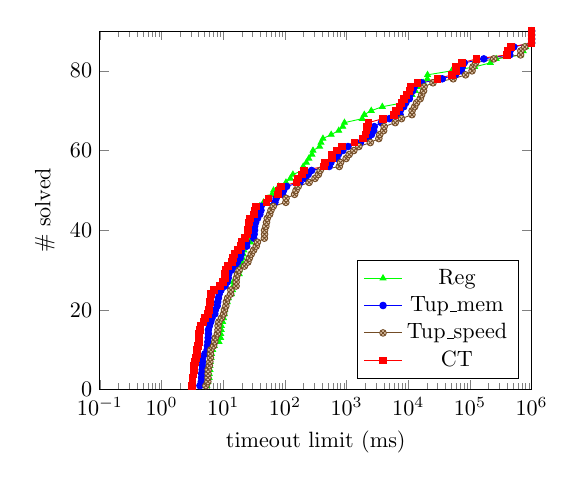
\begin{tikzpicture}[scale=0.8]
      \begin{axis}[
    xmode=log,
    ymin=0,ymax=90,
    xmin=0.1, xmax=1000000,
    every axis plot/.style={thin},
    xlabel={timeout limit (ms)},
    ylabel={\# solved},
    legend pos=south east
    % table/create on use/cumulative distribution/.style={
    %   create col/expr={\pgfmathaccuma + \thisrow{f(x)}}   
    % }
    ]
    \addplot 
    [mark=triangle*,
    mark size=1.5,
    mark options={solid},
    green] 
    coordinates {(5.389, 1)
(5.638, 2)
(5.908, 3)
(5.926, 4)
(6.086, 5)
(6.087, 6)
(6.166, 7)
(6.364, 8)
(6.469, 9)
(6.740, 10)
(7.148, 11)
(8.536, 12)
(9.080, 13)
(9.107, 14)
(9.303, 15)
(9.342, 16)
(9.805, 17)
(10.076, 18)
(10.428, 19)
(10.604, 20)
(10.907, 21)
(11.627, 22)
(12.123, 23)
(13.601, 24)
(14.151, 25)
(14.458, 26)
(14.490, 27)
(16.359, 28)
(18.190, 29)
(18.223, 30)
(18.413, 31)
(20.180, 32)
(20.506, 33)
(21.122, 34)
(21.643, 35)
(21.810, 36)
(27.563, 37)
(28.053, 38)
(28.274, 39)
(28.976, 40)
(30.018, 41)
(32.583, 42)
(32.814, 43)
(34.369, 44)
(38.523, 45)
(39.007, 46)
(44.977, 47)
(53.309, 48)
(61.875, 49)
(65.395, 50)
(79.428, 51)
(103.937, 52)
(122.565, 53)
(134.772, 54)
(193.149, 55)
(198.243, 56)
(223.375, 57)
(244.449, 58)
(274.390, 59)
(285.380, 60)
(365.560, 61)
(384.623, 62)
(413.842, 63)
(562.607, 64)
(746.251, 65)
(868.276, 66)
(924.223, 67)
(1793.623, 68)
(1937.966, 69)
(2509.726, 70)
(3797.584, 71)
(8373.485, 72)
(9593.391, 73)
(11531.366, 74)
(13031.885, 75)
(13941.016, 76)
(17694.770, 77)
(20392.242, 78)
(20545.405, 79)
(50620.318, 80)
(119540.736, 81)
(214612.883, 82)
(266484.425, 83)
(663627.605, 84)
(728667.872, 85)
(801665.108, 86)
(1000000.234, 87)
(1000000.344, 88)
(1000000.486, 89)
(1000000.515, 90)};

    \addplot 
    [blue,
    mark=*,
    mark size=1.5,
    mark options={solid}]
    coordinates {(4.188, 1)
(4.403, 2)
(4.451, 3)
(4.455, 4)
(4.562, 5)
(4.588, 6)
(4.619, 7)
(4.632, 8)
(5.046, 9)
(5.488, 10)
(5.538, 11)
(5.633, 12)
(5.705, 13)
(5.751, 14)
(5.756, 15)
(5.975, 16)
(6.278, 17)
(6.572, 18)
(7.295, 19)
(7.462, 20)
(7.979, 21)
(8.133, 22)
(8.358, 23)
(8.600, 24)
(9.209, 25)
(10.692, 26)
(11.548, 27)
(12.039, 28)
(12.248, 29)
(13.672, 30)
(15.880, 31)
(17.016, 32)
(18.711, 33)
(19.469, 34)
(19.729, 35)
(24.033, 36)
(24.051, 37)
(31.205, 38)
(31.687, 39)
(32.193, 40)
(32.329, 41)
(33.569, 42)
(35.982, 43)
(39.229, 44)
(40.895, 45)
(41.002, 46)
(68.982, 47)
(72.077, 48)
(91.486, 49)
(95.198, 50)
(106.573, 51)
(175.861, 52)
(214.260, 53)
(238.677, 54)
(271.193, 55)
(521.556, 56)
(557.425, 57)
(696.625, 58)
(735.011, 59)
(870.153, 60)
(1055.255, 61)
(1679.897, 62)
(2241.096, 63)
(2535.154, 64)
(2753.061, 65)
(2810.081, 66)
(3659.581, 67)
(4929.111, 68)
(7363.979, 69)
(7410.807, 70)
(8451.231, 71)
(9127.653, 72)
(10432.603, 73)
(10677.377, 74)
(11811.600, 75)
(12543.472, 76)
(16543.725, 77)
(35604.104, 78)
(58303.018, 79)
(72255.089, 80)
(75266.395, 81)
(80879.389, 82)
(167936.606, 83)
(442447.640, 84)
(447925.512, 85)
(514354.235, 86)
(1000001.142, 87)
(1000001.149, 88)
(1000001.277, 89)
(1000001.333, 90)};

    \addplot [brown!60!black,
    mark options={fill=brown!40},
    mark=otimes*,
    mark size=1.5]
    coordinates {(5.231, 1)
(5.629, 2)
(5.648, 3)
(5.663, 4)
(5.683, 5)
(5.943, 6)
(6.064, 7)
(6.179, 8)
(6.183, 9)
(6.295, 10)
(6.973, 11)
(7.284, 12)
(7.442, 13)
(8.037, 14)
(8.223, 15)
(8.238, 16)
(8.503, 17)
(9.384, 18)
(10.150, 19)
(10.464, 20)
(11.030, 21)
(11.224, 22)
(11.768, 23)
(13.192, 24)
(13.291, 25)
(16.148, 26)
(16.203, 27)
(16.372, 28)
(17.047, 29)
(18.087, 30)
(22.065, 31)
(25.084, 32)
(26.518, 33)
(28.470, 34)
(31.075, 35)
(34.278, 36)
(35.789, 37)
(46.424, 38)
(46.741, 39)
(46.749, 40)
(49.131, 41)
(50.337, 42)
(51.769, 43)
(56.622, 44)
(59.385, 45)
(64.673, 46)
(103.471, 47)
(104.380, 48)
(143.379, 49)
(151.391, 50)
(164.336, 51)
(246.920, 52)
(307.962, 53)
(349.129, 54)
(373.194, 55)
(761.064, 56)
(798.540, 57)
(984.391, 58)
(1100.413, 59)
(1311.163, 60)
(1581.664, 61)
(2426.014, 62)
(3330.803, 63)
(3451.164, 64)
(3985.165, 65)
(4060.894, 66)
(6149.120, 67)
(7773.303, 68)
(11478.659, 69)
(11534.975, 70)
(12707.939, 71)
(13658.601, 72)
(15631.173, 73)
(16480.122, 74)
(17709.931, 75)
(18042.131, 76)
(25195.852, 77)
(53588.555, 78)
(85036.871, 79)
(108170.261, 80)
(111741.798, 81)
(123479.329, 82)
(242924.139, 83)
(662412.696, 84)
(668282.082, 85)
(773006.352, 86)
(1000000.222, 87)
(1000000.350, 88)
(1000000.409, 89)
(1000001.208, 90)};

    \addplot 
    [red,
    mark size=1.5,
    mark=square*]
    coordinates {(3.077, 1)
(3.159, 2)
(3.165, 3)
(3.290, 4)
(3.360, 5)
(3.387, 6)
(3.499, 7)
(3.591, 8)
(3.773, 9)
(3.788, 10)
(3.878, 11)
(3.996, 12)
(3.998, 13)
(4.030, 14)
(4.235, 15)
(4.270, 16)
(4.806, 17)
(4.996, 18)
(5.677, 19)
(5.849, 20)
(5.952, 21)
(6.121, 22)
(6.164, 23)
(6.365, 24)
(7.079, 25)
(8.883, 26)
(9.951, 27)
(10.577, 28)
(10.722, 29)
(10.853, 30)
(11.910, 31)
(13.844, 32)
(14.533, 33)
(15.242, 34)
(17.301, 35)
(19.220, 36)
(19.624, 37)
(22.571, 38)
(24.789, 39)
(24.978, 40)
(25.692, 41)
(25.836, 42)
(27.326, 43)
(31.105, 44)
(32.150, 45)
(33.871, 46)
(50.022, 47)
(53.705, 48)
(77.777, 49)
(78.665, 50)
(86.000, 51)
(153.424, 52)
(163.326, 53)
(186.857, 54)
(205.347, 55)
(431.945, 56)
(447.896, 57)
(579.321, 58)
(582.538, 59)
(697.105, 60)
(845.847, 61)
(1342.019, 62)
(1841.060, 63)
(2032.310, 64)
(2086.544, 65)
(2136.864, 66)
(2259.967, 67)
(3859.192, 68)
(5928.297, 69)
(6294.023, 70)
(7189.658, 71)
(7718.920, 72)
(8552.721, 73)
(9394.659, 74)
(10400.047, 75)
(10914.835, 76)
(14065.923, 77)
(29727.731, 78)
(50913.845, 79)
(58766.196, 80)
(59010.473, 81)
(73352.608, 82)
(127355.852, 83)
(398786.693, 84)
(405416.242, 85)
(466149.784, 86)
(1000000.184, 87)
(1000000.216, 88)
(1000000.280, 89)
(1000000.721, 90)};
    \legend{Reg,Tup\_mem,Tup\_speed,CT}
  \end{axis}

    \end{tikzpicture}
    \vfill
    \caption{\textbf{Geom}. The 100 instances of this benchmark
    contain binary constraints. The variable domains are
    1..20.}
    \vspace{\baselineskip}
  \end{minipage}\qquad

\end{figure}

\newpage

\begin{figure}
  \begin{minipage}[b][10cm][s]{0.45\textwidth}
    \centering
    \vfill
    \begin{tikzpicture}[scale=0.8]
      \begin{axis}[
    xmode=log,
    ymin=0,ymax=13,
    xmin=0.1, xmax=1000000,
    every axis plot/.style={thin},
    xlabel={timeout limit (ms)},
    ylabel={\# solved},
    legend pos=south east
    % table/create on use/cumulative distribution/.style={
    %   create col/expr={\pgfmathaccuma + \thisrow{f(x)}}   
    % }
    ]
    \addplot 
    [mark=triangle*,
    mark size=1.5,
    mark options={solid},
    green] 
    coordinates {(25692.763, 1)
(52566.138, 2)
(108946.436, 3)
(221877.475, 4)
(464154.393, 5)
(959255.963, 6)
(1000000.112, 7)
(1000000.119, 8)
(1000000.125, 9)
(1000000.129, 10)
(1000000.202, 11)
(1000000.206, 12)
(1000000.220, 13)};

    \addplot 
    [blue,
    mark=*,
    mark size=1.5,
    mark options={solid}]
    coordinates {(24930.451, 1)
(51072.293, 2)
(104903.803, 3)
(218612.431, 4)
(452788.242, 5)
(938091.619, 6)
(1000000.148, 7)
(1000000.149, 8)
(1000000.179, 9)
(1000000.201, 10)
(1000000.213, 11)
(1000000.232, 12)
(1000000.236, 13)};

    \addplot [brown!60!black,
    mark options={fill=brown!40},
    mark=otimes*,
    mark size=1.5]
    table {(32168.167, 1)
(67198.233, 2)
(137576.561, 3)
(283937.740, 4)
(592360.368, 5)
(1000000.108, 6)
(1000000.110, 7)
(1000000.115, 8)
(1000000.116, 9)
(1000000.125, 10)
(1000000.180, 11)
(1000000.190, 12)
(1000000.202, 13)};

    \addplot 
    [red,
    mark size=1.5,
    mark=square*]
    table {(21084.624, 1)
(42987.264, 2)
(88183.028, 3)
(183554.060, 4)
(374851.071, 5)
(785860.510, 6)
(1000000.112, 7)
(1000000.115, 8)
(1000000.120, 9)
(1000000.183, 10)
(1000000.200, 11)
(1000000.202, 12)
(1061960.067, 13)};
    \legend{Reg,Tup\_mem,Tup\_speed,CT}
  \end{axis}

    \end{tikzpicture}
    \vfill
    \caption{\textbf{Dubois}. The 12 instances of this benchmark
      contain two constraints each, of arity 3.
      All variables are 0/1.}
    \vspace{\baselineskip}
  \end{minipage}\qquad

\end{figure}

\newpage

\begin{figure}
  \begin{minipage}[b][10cm][s]{0.45\textwidth}
    \centering
    \vfill
    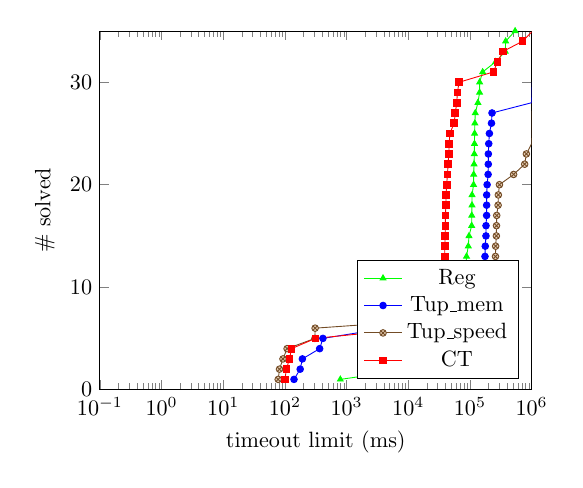
\begin{tikzpicture}[scale=0.8]
      \begin{axis}[
    xmode=log,
    ymin=0,ymax=35,
    xmin=0.1, xmax=1000000,
    every axis plot/.style={thin},
    xlabel={timeout limit (ms)},
    ylabel={\# solved},
    legend pos=south east
    % table/create on use/cumulative distribution/.style={
    %   create col/expr={\pgfmathaccuma + \thisrow{f(x)}}   
    % }
    ]
    \addplot 
    [mark=triangle*,
    mark size=1.5,
    mark options={solid},
    green] 
    coordinates {(791.560, 1)
(11472.600, 2)
(14766.696, 3)
(15745.163, 4)
(26862.099, 5)
(31778.084, 6)
(72448.015, 7)
(80752.168, 8)
(82923.009, 9)
(83683.963, 10)
(84465.445, 11)
(85764.561, 12)
(88032.555, 13)
(94011.079, 14)
(96560.156, 15)
(106648.859, 16)
(107056.591, 17)
(107933.416, 18)
(108210.305, 19)
(114497.218, 20)
(114966.358, 21)
(116658.706, 22)
(117735.741, 23)
(118508.245, 24)
(119006.430, 25)
(120178.594, 26)
(122120.270, 27)
(134711.654, 28)
(143405.319, 29)
(143582.718, 30)
(160788.320, 31)
(261709.502, 32)
(374501.791, 33)
(379347.315, 34)
(540015.740, 35)};

    \addplot 
    [blue,
    mark=*,
    mark size=1.5,
    mark options={solid}]
    coordinates {(140.425, 1)
(176.917, 2)
(192.112, 3)
(365.981, 4)
(413.133, 5)
(4403.296, 6)
(39876.347, 7)
(92306.099, 8)
(167189.458, 9)
(169366.958, 10)
(170556.481, 11)
(173851.037, 12)
(175430.330, 13)
(177265.457, 14)
(181905.169, 15)
(182312.517, 16)
(186399.578, 17)
(186652.401, 18)
(186832.299, 19)
(189971.439, 20)
(197152.408, 21)
(198415.969, 22)
(198894.284, 23)
(201831.845, 24)
(206792.806, 25)
(223634.515, 26)
(228125.105, 27)
(1001453.819, 28)
(1004586.749, 29)
(1020114.517, 30)
(1167495.643, 31)
(1316010.414, 32)
(1399844.041, 33)
(1422830.720, 34)
(1553624.496, 35)};

    \addplot [brown!60!black,
    mark options={fill=brown!40},
    mark=otimes*,
    mark size=1.5]
    coordinates {(77.848, 1)
(81.738, 2)
(93.013, 3)
(108.475, 4)
(306.721, 5)
(309.048, 6)
(71781.939, 7)
(119555.503, 8)
(232959.976, 9)
(235395.918, 10)
(237247.816, 11)
(247450.645, 12)
(259525.670, 13)
(261038.714, 14)
(268346.434, 15)
(269506.659, 16)
(271797.636, 17)
(286253.613, 18)
(288902.149, 19)
(300957.270, 20)
(510582.087, 21)
(771478.727, 22)
(822435.981, 23)
(1000367.652, 24)
(1005161.590, 25)
(1010019.345, 26)
(1010418.164, 27)
(1022093.039, 28)
(1029891.832, 29)
(1031150.393, 30)
(1034813.269, 31)
(1054519.771, 32)
(1073321.307, 33)
(1142503.375, 34)
(1301096.751, 35)};

    \addplot 
    [red,
    mark size=1.5,
    mark=square*]
    coordinates {(100.268, 1)
(105.476, 2)
(118.901, 3)
(127.592, 4)
(313.306, 5)
(13094.233, 6)
(19436.829, 7)
(34008.560, 8)
(35649.282, 9)
(36572.672, 10)
(36586.778, 11)
(38788.690, 12)
(39051.053, 13)
(39170.191, 14)
(39702.088, 15)
(39815.587, 16)
(40011.946, 17)
(40780.574, 18)
(40946.927, 19)
(41904.986, 20)
(43203.913, 21)
(44258.721, 22)
(45394.073, 23)
(46118.992, 24)
(47174.176, 25)
(55599.614, 26)
(57777.455, 27)
(61166.183, 28)
(62548.310, 29)
(66755.839, 30)
(239564.852, 31)
(281010.056, 32)
(343727.677, 33)
(713034.541, 34)
(1040781.786, 35)};
    \legend{Reg,Tup\_mem,Tup\_speed,CT}
  \end{axis}

    \end{tikzpicture}
    \vfill
    \caption{\textbf{BDD Large}.
      The 35 instances of this benchmark contain constraints
      of arity 15. The variables are 0/1.}
    \vspace{\baselineskip}
  \end{minipage}\qquad
\end{figure}






% \paragraph{Crosswords}
% Crosswords_lexVg
% Crosswords_wordsPuzzle
% Crosswords_wordsVg

% \paragraph{Travelling Salesman Problem}
% TSP_20
% TSP_25
% TSP_Quat_20


% a10
% a5
% aim-100-pos
% aim-200-pos
% aim-50-pos
% bddLarge
% bddSmall
% dubois
% geom
% k5_n10_d10_m15_p08

% \paragraph{Kakuro}
% kakuroext_easy
% kakuroext_hard
% kakuroext_medium

% \paragraph{Langford}
% langford2
% langford3
% langford4

% \paragraph{MDD}
% mdd05
% mdd07
% mdd09


% modRenault

% \paragraph{Nonograms}
% nonograms

% pigeonsplus

% \paragraph{Randomised instances}
% randsJC10000
% randsJC2500
% randsJC5000
% randsJC7500

% ssa

% \begin{table}[t] \tiny
%   \centering
%   \begin{tabular}{rrrrrrr}  % right alignment --> decimal point alignment
%     $n$ & $runtime_g$ & $fail_g$ & $nprops_g$ & $runtime_c$ & $fail_c$ & $nprops_c$ \\
%     \midrule
%     0 & 0.119 & 7 & 4679 & 0.366 & 6 & 4474 \\
1 & 0.085 & 2 & 1780 & 0.166 & 11 & 5119 \\
2 & 0.073 & 1 & 1684 & 0.197 & 0 & 1241 \\
3 & 0.052 & 6 & 2065 & 0.137 & 6 & 2266 \\
4 & 0.033 & 0 & 845 & 0.064 & 0 & 850 \\
5 & 0.087 & 0 & 1275 & 0.169 & 0 & 1260 \\
6 & 0.082 & 7 & 3952 & 0.136 & 6 & 3967 \\
7 & 0.077 & 3 & 2304 & 0.102 & 4 & 2460 \\
8 & 0.051 & 2 & 1281 & 0.103 & 2 & 1306 \\
9 & 0.034 & 0 & 825 & 0.072 & 0 & 875 \\
10 & 1.227 & 16 & 171162 & 1.112 & 46 & 298509 \\
11 & 1.399 & 41 & 410228 & 1.063 & 21 & 230481 \\
12 & 1.067 & 3 & 95731 & 1.217 & 71 & 405968 \\
13 & 2.342 & 381 & 1700606 & \Timeout & 147028 & 603399614 \\
14 & 0.978 & 25 & 191179 & 0.873 & 10 & 124704 \\
15 & 3.154 & 245 & 1146764 & 2.368 & 178 & 879023 \\
16 & 2.910 & 185 & 992421 & 1.710 & 152 & 734316 \\
17 & 1.006 & 11 & 136377 & 1.119 & 16 & 128781 \\
18 & 1.052 & 7 & 108977 & 0.958 & 11 & 122557 \\
19 & 3.012 & 166 & 1083832 & 2.131 & 219 & 1381581 \\
20 & 2.690 & 32 & 319505 & 1.858 & 21 & 332253 \\
21 & 2.818 & 61 & 766182 & 5.233 & 1091 & 8287668 \\
22 & \Timeout & 28601 & 171635604 & \Timeout & 69906 & 464113700 \\
23 & 2.475 & 53 & 616660 & \Timeout & 61878 & 414187753 \\
24 & 3.513 & 177 & 841650 & 1.681 & 13 & 324284 \\
25 & 2.441 & 18 & 301053 & 1.694 & 19 & 339487 \\
26 & 2.415 & 25 & 374594 & 1.711 & 16 & 326141 \\
27 & 2.215 & 7 & 264087 & 2.238 & 5 & 270104 \\
28 & 1.919 & 14 & 272577 & 1.804 & 13 & 273908 \\
29 & 2.228 & 8 & 212822 & 1.936 & 6 & 221706 \\
30 & \Timeout & 18058 & 119444044 & \Timeout & 47925 & 497445022 \\
31 & \Timeout & 23283 & 178289620 & 2.670 & 30 & 532937 \\
32 & 4.870 & 63 & 913320 & \Timeout & 166635 & 858563943 \\
33 & \Timeout & 15181 & 147948821 & \Timeout & 67148 & 763053956 \\
34 & \Timeout & 39057 & 303289935 & 9.809 & 1726 & 14322164 \\
35 & 4.376 & 52 & 904626 & \Timeout & 117958 & 1084029060 \\
36 & 4.396 & 114 & 1628267 & 4.487 & 197 & 1934868 \\
37 & \Timeout & 21286 & 132575730 & 3.146 & 35 & 542375 \\
38 & 4.577 & 79 & 1045936 & 3.162 & 51 & 856676 \\
39 & \Timeout & 9040 & 99188489 & \Timeout & 39272 & 399951117 \\
40 & 2.930 & 1 & 34787 & 2.915 & 1 & 69542 \\
41 & 5.303 & 40 & 790942 & 3.325 & 44 & 834269 \\
42 & \Timeout & 12605 & 148700057 & \Timeout & 42626 & 406830329 \\
43 & 9.819 & 361 & 5325834 & 6.875 & 373 & 5490353 \\
44 & 5.528 & 116 & 1336494 & 4.065 & 37 & 789395 \\
45 & \Timeout & 8415 & 111542169 & \Timeout & 27352 & 334646024 \\
46 & 6.539 & 248 & 2498691 & 4.149 & 80 & 1240475 \\
47 & \Timeout & 22179 & 282707631 & \Timeout & 34120 & 451342876 \\
48 & \Timeout & 19778 & 164139781 & \Timeout & 51875 & 649868285 \\
49 & \Timeout & 15047 & 208250589 & \Timeout & 32003 & 508583392 \\
50 & 0.021 & 0 & 24 & 0.021 & 0 & 29 \\
51 & 0.076 & 0 & 192 & 0.054 & 0 & 209 \\
52 & 0.055 & 0 & 521 & 0.062 & 0 & 525 \\
53 & 0.366 & 6 & 2065 & 0.235 & 6 & 2266 \\
54 & 0.144 & 0 & 1030 & 0.416 & 0 & 988 \\
55 & 0.155 & 2 & 1699 & 0.333 & 2 & 1766 \\
56 & 0.212 & 0 & 2499 & 0.284 & 0 & 2477 \\
57 & 0.279 & 0 & 4201 & 0.226 & 0 & 4440 \\
58 & 0.359 & 0 & 3124 & 0.303 & 0 & 3259 \\
59 & 0.248 & 0 & 4518 & 0.257 & 0 & 4559 \\
60 & 0.246 & 2 & 4170 & 0.301 & 0 & 3489 \\
61 & 0.229 & 0 & 7555 & 0.223 & 1 & 8870 \\
62 & 0.303 & 2 & 12954 & 0.416 & 3 & 13698 \\
63 & 0.378 & 1 & 10738 & 0.603 & 1 & 10691 \\
64 & 0.459 & 2 & 28017 & 0.638 & 12 & 51083 \\
65 & 0.721 & 7 & 57191 & 0.888 & 6 & 54937 \\
66 & 1.134 & 12 & 127865 & 1.490 & 6 & 107939 \\
67 & 1.014 & 10 & 124827 & 0.877 & 13 & 117966 \\
68 & 1.499 & 8 & 111993 & 1.572 & 6 & 114614 \\
69 & 0.351 & 0 & 6613 & 0.310 & 0 & 6631 \\
70 & 0.693 & 20 & 82813 & 0.882 & 16 & 87958 \\
71 & 0.588 & 12 & 92658 & 0.932 & 12 & 98391 \\
 % let your experiment script write directly
%                             % into this file, making sure every number
%                             % in a column has the _same_ number of decimals
%   \end{tabular}
%   \caption{}
%   \label{tab:res:sat}
% \end{table}


\subsection{Discussion}
\label{evaluation:discussion}



\section{Conclusions and Future Work}
\label{conclusions}

\bibliographystyle{abbrv}
\bibliography{astra,mybib}

\appendix
\section{Source Code}
\label{sec:source-code}


This appendix presents the source code for the implementation described in \Chapref{sec:implementation}.





\end{document}

%%% Local Variables:
%%% mode: latex
%%% TeX-master: t
%%% End:

% OscaR source code:
% https://bitbucket.org/oscarlib/oscar/src/40e25aafba8f9b0ab06029449350a2a9d1614854/oscar-algo/src/main/scala/oscar/algo/reversible/ReversibleSparseBitSet.scala?at=dev&fileviewer=file-view-default
% https://bitbucket.org/oscarlib/oscar/src/40e25aafba8f9b0ab06029449350a2a9d1614854/oscar-cp/src/main/scala/oscar/cp/constraints/tables/TableCT.scala?at=dev&fileviewer=file-view-default3

% course note in constraint programming
% http://user.it.uu.se/~pierref/courses/COCP/slides/CourseNotes.pdf

% M-x reftex-parse-all
% F1 b
% M-x customize-group reftex

% Hash Functions
% https://en.wikipedia.org/wiki/Pairing_function
% https://www.cs.hmc.edu/~geoff/classes/hmc.cs070.200101/homework10/hashfuncs.html
% http://stackoverflow.com/questions/37918951/what-is-a-minimal-hash-function-for-a-pair-of-ints-that-has-low-chance-of-collis

